\documentclass[10pt]{article}

\usepackage[a4paper,margin=0.65in]{geometry}
\usepackage{amsmath,amssymb}
\usepackage{graphicx}
\usepackage{booktabs}
\usepackage{array}
\usepackage{float}
\usepackage{hyperref}
\usepackage{enumitem}
\usepackage{xcolor}
\usepackage{tikz}
\usetikzlibrary{positioning,arrows.meta,shapes.geometric}

\setlist{nosep,leftmargin=*}
\renewcommand{\arraystretch}{1.2}
\setlength{\parindent}{0pt}
\setlength{\parskip}{2pt}

\tikzset{
layer/.style={
draw,
rounded corners,
minimum width=1.5cm,
minimum height=0.6cm,
align=center,
fill=blue!10,
font=\scriptsize
},
arrow/.style={
-{Latex[length=2mm]},
thin
}
}

\begin{document}

%%%%%%%%%%%%%%%%%%%%%%%%%%%%%%%%%%%%%%%%%%%%%%%%%%%%%%%%%%%%
% TITLE
%%%%%%%%%%%%%%%%%%%%%%%%%%%%%%%%%%%%%%%%%%%%%%%%%%%%%%%%%%%%

\begin{center}

{\large\textbf{Shiv Nadar University Chennai}}

\vspace{2mm}

{\normalsize\textbf{CS3807 -- Deep Learning Laboratory}}

\vspace{2mm}

{\large\textbf{Experiment 5}}

\vspace{1mm}

{\normalsize\textbf{Comprehensive Study of CNN Training, Regularization,}}

{\normalsize\textbf{Optimization, Hyperparameter Tuning, Transfer Learning}}

{\normalsize\textbf{and Cross-Validation}}

\end{center}

\vspace{3mm}

\begin{tabular}{|p{3.4cm}|p{9.0cm}|p{1.4cm}|}
\hline
Degree \& Branch &
B.Tech Artificial Intelligence \& Data Science &
Semester V\\
\hline
Subject Code \& Name &
CS3807 -- Deep Learning Laboratory &
AY: 2026--27\\
\hline
\end{tabular}

%%%%%%%%%%%%%%%%%%%%%%%%%%%%%%%%%%%%%%%%%%%%%%%%%%%%%%%%%%%%
\section{Objective}

The objective of this experiment is to systematically study the effect of
weight initialization, regularization, optimization algorithms, CNN
hyperparameters, transfer learning, fine-tuning and cross-validation on
image classification performance.

The experiment uses a single CNN architecture, MobileNetV2, and the
Oxford-IIIT Pet dataset. Students will analyze the effect of individual
design choices using training/validation curves and finally select a
suitable configuration using 5-fold cross-validation.

%%%%%%%%%%%%%%%%%%%%%%%%%%%%%%%%%%%%%%%%%%%%%%%%%%%%%%%%%%%%
\section{Learning Outcomes}

After completing this experiment, students will be able to:

\begin{itemize}
\item explain different weight initialization strategies;
\item identify and analyze overfitting using training and validation curves;
\item compare SGD, Momentum, RMSProp and Adam;
\item explain CNN hyperparameters such as kernel size, stride, padding and pooling;
\item understand Batch Normalization and Dropout;
\item perform transfer learning and fine-tuning using MobileNetV2;
\item tune important training hyperparameters;
\item apply 5-fold cross-validation for model selection; and
\item justify the final model using accuracy, variability and computational cost.
\end{itemize}

%%%%%%%%%%%%%%%%%%%%%%%%%%%%%%%%%%%%%%%%%%%%%%%%%%%%%%%%%%%%
\section{Dataset and Experimental Setup}

\textbf{Dataset: Oxford-IIIT Pet Dataset}

The Oxford-IIIT Pet Dataset contains images of cats and dogs belonging
to 37 breeds. The images are RGB and have different spatial dimensions.
For this experiment, all images are resized to

\[
224\times224\times3.
\]

The dataset is suitable for demonstrating transfer learning using
ImageNet-pretrained CNNs.

\textbf{Experimental considerations:}

\begin{itemize}
\item Use RGB images resized to $224\times224$.
\item Normalize the input images according to the pretrained model requirements.
\item Maintain separate training, validation and test data.
\item The test set must remain untouched during hyperparameter selection.
\item Use MobileNetV2 because it is computationally lighter than many
large CNN architectures and is more suitable for CPU-based laboratory work.
\end{itemize}

%%%%%%%%%%%%%%%%%%%%%%%%%%%%%%%%%%%%%%%%%%%%%%%%%%%%%%%%%%%%
\section{MobileNetV2 Architecture}

MobileNetV2 is a lightweight CNN architecture designed to reduce
computational complexity while maintaining good image representation.

Its important components include:

\begin{itemize}
\item depthwise convolution;
\item pointwise $1\times1$ convolution;
\item inverted residual blocks;
\item linear bottlenecks;
\item batch normalization; and
\item ReLU6 activation.
\end{itemize}

A simplified representation is:

\begin{center}
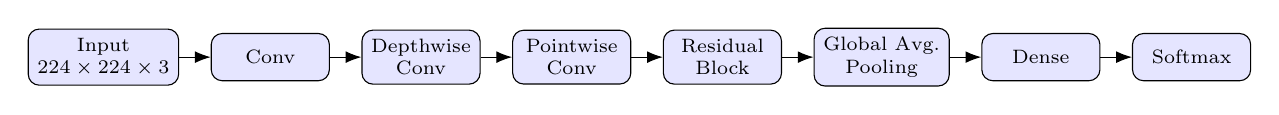
\begin{tikzpicture}[node distance=4mm]

\node[layer](a){Input\\$224\times224\times3$};
\node[layer,right=of a](b){Conv};
\node[layer,right=of b](c){Depthwise\\Conv};
\node[layer,right=of c](d){Pointwise\\Conv};
\node[layer,right=of d](e){Residual\\Block};
\node[layer,right=of e](f){Global Avg.\\Pooling};
\node[layer,right=of f](g){Dense};
\node[layer,right=of g](h){Softmax};

\foreach \x/\y in {a/b,b/c,c/d,d/e,e/f,f/g,g/h}
\draw[arrow](\x)--(\y);

\end{tikzpicture}
\end{center}

\textbf{Note:} The above diagram is a simplified conceptual representation
rather than the complete MobileNetV2 architecture.

%%%%%%%%%%%%%%%%%%%%%%%%%%%%%%%%%%%%%%%%%%%%%%%%%%%%%%%%%%%%
\section{Weight Initialization}

Weight initialization determines the initial values of trainable weights
before training begins. A suitable initialization can improve convergence
and reduce problems such as vanishing or exploding activations.

Students should investigate:

\begin{itemize}
\item Zero initialization
\item Random initialization
\item Xavier/Glorot initialization
\item He initialization
\end{itemize}

\subsection*{Expected Analysis}

Students should compare the initialization strategies using:

\textbf{Plot 1: Training Loss vs. Epoch}

\begin{itemize}
\item X-axis: Epoch
\item Y-axis: Training Loss
\item Plot one curve for each initialization method.
\end{itemize}

\textbf{Plot 2: Validation Accuracy vs. Epoch}

\begin{itemize}
\item X-axis: Epoch
\item Y-axis: Validation Accuracy (\%)
\item Plot one curve for each initialization method.
\end{itemize}

Students should identify which initialization gives faster and more
stable convergence.

%%%%%%%%%%%%%%%%%%%%%%%%%%%%%%%%%%%%%%%%%%%%%%%%%%%%%%%%%%%%
\section{Regularization and Overfitting}

Overfitting occurs when a model performs very well on the training data
but generalizes poorly to unseen data.

Students should compare:

\begin{itemize}
\item No regularization
\item L2 regularization
\item Dropout
\item Batch Normalization
\end{itemize}

\subsection*{Expected Plots}

\textbf{Plot 3: Training and Validation Accuracy vs. Epoch}

\begin{itemize}
\item X-axis: Epoch
\item Y-axis: Accuracy (\%)
\item Plot separate curves for training and validation accuracy.
\end{itemize}

Students should identify the generalization gap.

\textbf{Plot 4: Training and Validation Loss vs. Epoch}

\begin{itemize}
\item X-axis: Epoch
\item Y-axis: Loss
\item Plot training and validation loss.
\end{itemize}

Students should identify whether validation loss begins to increase while
training loss continues to decrease.

%%%%%%%%%%%%%%%%%%%%%%%%%%%%%%%%%%%%%%%%%%%%%%%%%%%%%%%%%%%%
\section{Batch Normalization}

Batch Normalization normalizes activations within a mini-batch during
training.

For a mini-batch

\[
x_1,x_2,\ldots,x_m,
\]

the batch mean is

\[
\mu_B=\frac{1}{m}\sum_{i=1}^{m}x_i
\]

and the batch variance is

\[
\sigma_B^2=
\frac{1}{m}\sum_{i=1}^{m}(x_i-\mu_B)^2.
\]

The normalized activation is

\[
\hat{x}_i=
\frac{x_i-\mu_B}
{\sqrt{\sigma_B^2+\epsilon}}.
\]

The final output is

\[
y_i=\gamma\hat{x}_i+\beta,
\]

where $\gamma$ and $\beta$ are learnable parameters.

\subsection*{Numerical Example}

Consider

\[
x=[2,4,6,8].
\]

The mean is

\[
\mu_B=\frac{2+4+6+8}{4}=5.
\]

The variance is

\[
\sigma_B^2=
\frac{(2-5)^2+(4-5)^2+(6-5)^2+(8-5)^2}{4}
=5.
\]

Therefore,

\[
\sqrt{5}\approx2.236.
\]

Ignoring the very small $\epsilon$,

\[
\hat{x}_1=\frac{2-5}{2.236}\approx-1.342,
\]

\[
\hat{x}_2=\frac{4-5}{2.236}\approx-0.447,
\]

\[
\hat{x}_3=\frac{6-5}{2.236}\approx0.447,
\]

\[
\hat{x}_4=\frac{8-5}{2.236}\approx1.342.
\]

Hence,

\[
\boxed{
\hat{x}\approx[-1.342,-0.447,0.447,1.342]
}
\]

If $\gamma=1$ and $\beta=0$, these are the final outputs.

\textbf{Inference:} Batch Normalization produces approximately
zero-centred and unit-scaled activations for this mini-batch. The
learnable $\gamma$ and $\beta$ allow the network to learn an appropriate
scale and shift.

\textbf{Plot 5: With vs. Without Batch Normalization}

\begin{itemize}
\item X-axis: Epoch
\item Y-axis: Validation Accuracy (\%)
\item Compare two curves: With BN and Without BN.
\end{itemize}

%%%%%%%%%%%%%%%%%%%%%%%%%%%%%%%%%%%%%%%%%%%%%%%%%%%%%%%%%%%%
\section{Optimization Algorithms}

Students should compare the following optimization methods:

\begin{itemize}
\item SGD
\item Momentum
\item RMSProp
\item Adam
\end{itemize}

The objective is to study convergence speed, stability and final
validation performance.

\textbf{Plot 6: Training Loss vs. Epoch for Different Optimizers}

\begin{itemize}
\item X-axis: Epoch
\item Y-axis: Training Loss
\item One curve for each optimizer.
\end{itemize}

\textbf{Plot 7: Validation Accuracy vs. Epoch for Different Optimizers}

\begin{itemize}
\item X-axis: Epoch
\item Y-axis: Validation Accuracy (\%)
\item One curve for each optimizer.
\end{itemize}



%%%%%%%%%%%%%%%%%%%%%%%%%%%%%%%%%%%%%%%%%%%%%%%%%%%%%%%%%%%%
\section{CNN Hyperparameter Tuning}

The following hyperparameters should be investigated:

\begin{center}
\begin{tabular}{|l|l|}
\hline
Hyperparameter & Suggested Values\\
\hline
Learning Rate & $0.001,\;0.0001$\\
Batch Size & 16, 32, 64\\
Dropout Rate & 0, 0.25, 0.5\\
Optimizer & SGD, Adam\\
Fine-Tuning Learning Rate & $10^{-4},10^{-5}$\\
Frozen Layers & Frozen base / Partial unfreezing\\
\hline
\end{tabular}
\end{center}

For CNN concepts, students should also understand:

\begin{itemize}
\item kernel/filter;
\item stride;
\item padding;
\item pooling;
\item number of channels; and
\item depthwise separable convolution.
\end{itemize}

For a convolution operation, the output dimension can be calculated as

\[
O=
\left\lfloor
\frac{N+2P-K}{S}
\right\rfloor+1,
\]

where $N$ is input size, $K$ is kernel size, $P$ is padding and $S$ is
stride.

\textbf{Experimental rule:} During a controlled hyperparameter study,
change one hyperparameter at a time while keeping the remaining settings
fixed.

\textbf{Plot 8: Learning Rate vs. Validation Accuracy}

\begin{itemize}
\item X-axis: Learning Rate
\item Y-axis: Validation Accuracy (\%)
\end{itemize}

\textbf{Plot 9: Batch Size vs. Validation Accuracy}

\begin{itemize}
\item X-axis: Batch Size
\item Y-axis: Validation Accuracy (\%)
\end{itemize}

\textbf{Plot 10: Dropout Rate vs. Validation Accuracy}

\begin{itemize}
\item X-axis: Dropout Rate
\item Y-axis: Validation Accuracy (\%)
\end{itemize}

%%%%%%%%%%%%%%%%%%%%%%%%%%%%%%%%%%%%%%%%%%%%%%%%%%%%%%%%%%%%
\section{Transfer Learning and Fine-Tuning}

MobileNetV2 pretrained on ImageNet should be used.

\subsection*{Case A: Feature Extraction}

\[
\text{Pretrained MobileNetV2}
\rightarrow
\text{Freeze Base}
\rightarrow
\text{New Classifier}
\]

The pretrained convolutional layers are frozen and only the newly added
classification layers are trained.

\subsection*{Case B: Fine-Tuning}

\[
\text{Pretrained MobileNetV2}
\rightarrow
\text{Unfreeze Selected Layers}
\rightarrow
\text{Small Learning Rate}
\]

The upper layers of the pretrained network are unfrozen and trained with
a smaller learning rate.

\textbf{Plot 11: Feature Extraction vs. Fine-Tuning}

\begin{itemize}
\item X-axis: Epoch
\item Y-axis: Validation Accuracy (\%)
\item Two curves: Feature Extraction and Fine-Tuning.
\end{itemize}

\textbf{Plot 12: Training and Validation Loss}

Students should compare the loss curves before and after fine-tuning.

\textbf{Discussion:} Explain why fine-tuning normally requires a smaller
learning rate than training a newly initialized classifier.

%%%%%%%%%%%%%%%%%%%%%%%%%%%%%%%%%%%%%%%%%%%%%%%%%%%%%%%%%%%%
\section{K-Fold Cross-Validation}

After the individual studies, select 3--4 promising configurations.

Use 5-fold cross-validation on the training data.

For $K=5$,

\[
\bar{A}=
\frac{1}{5}\sum_{i=1}^{5}A_i
\]

and

\[
SD=
\sqrt{
\frac{1}{5}
\sum_{i=1}^{5}(A_i-\bar{A})^2
}.
\]

Report the result as

\[
\boxed{\bar{A}\pm SD}.
\]

The independent test set must not be used during hyperparameter selection.


\textbf{Plot 13: 5-Fold Cross-Validation Accuracy}

\begin{itemize}
\item X-axis: Hyperparameter Configuration
\item Y-axis: Mean Validation Accuracy (\%)
\item Include standard-deviation error bars.
\end{itemize}

Students should discuss both mean performance and variability.

%%%%%%%%%%%%%%%%%%%%%%%%%%%%%%%%%%%%%%%%%%%%%%%%%%%%%%%%%%%%
\section{Final Model Evaluation}

After selecting the best configuration using cross-validation:

\begin{enumerate}
\item Retrain the selected configuration using the complete training data.
\item Keep the independent test set untouched until this stage.
\item Evaluate the final model on the test set.
\end{enumerate}

\textbf{Plot 14: Confusion Matrix}

Students should identify:

\begin{itemize}
\item the best classified classes;
\item the most frequently confused classes; and
\item possible visual reasons for misclassification.
\end{itemize}

\textbf{Optional Plot 15: Misclassified Images}

Display representative incorrectly classified images and provide a
brief explanation for each.

%%%%%%%%%%%%%%%%%%%%%%%%%%%%%%%%%%%%%%%%%%%%%%%%%%%%%%%%%%%%
\section{Source Code}

\noindent\textbf{Source:} Github\\
\noindent\textbf{Github Repository Link:}

\url{https://github.com/ssvibitha/DeepLearningLab_2026-27/blob/main/Lab5_MobileNetV2/DL_Lab5.ipynb}


%%%%%%%%%%%%%%%%%%%%%%%%%%%%%%%%%%%%%%%%%%%%%%%%%%%%%%%%%%%%
\section{Plots and Inference}
\begin{enumerate}
    \item\textbf{Sample Oxford-IIIT Pet Dataset images}
        \begin{figure}[H]
        \centering
        
\includegraphics[width=0.5\textwidth]{Images/SampleImages.png}
        \caption{Sample Images}
        \label{fig:SampleImages}
    \end{figure}
    \noindent\textbf{Inference:}\\
    The figures show sample images from the Oxford IIIT Pet Dataset. The dataset contains 7390 images.
    The images belong to 37 different breeds of cats and dogs. 
    Each image is 224 x 224 pixels and contains three color channels (RGB)

    \clearpage

    \item\textbf{Weight Initialization: Training Loss vs Epoch}
        \begin{figure}[H]
        \centering
        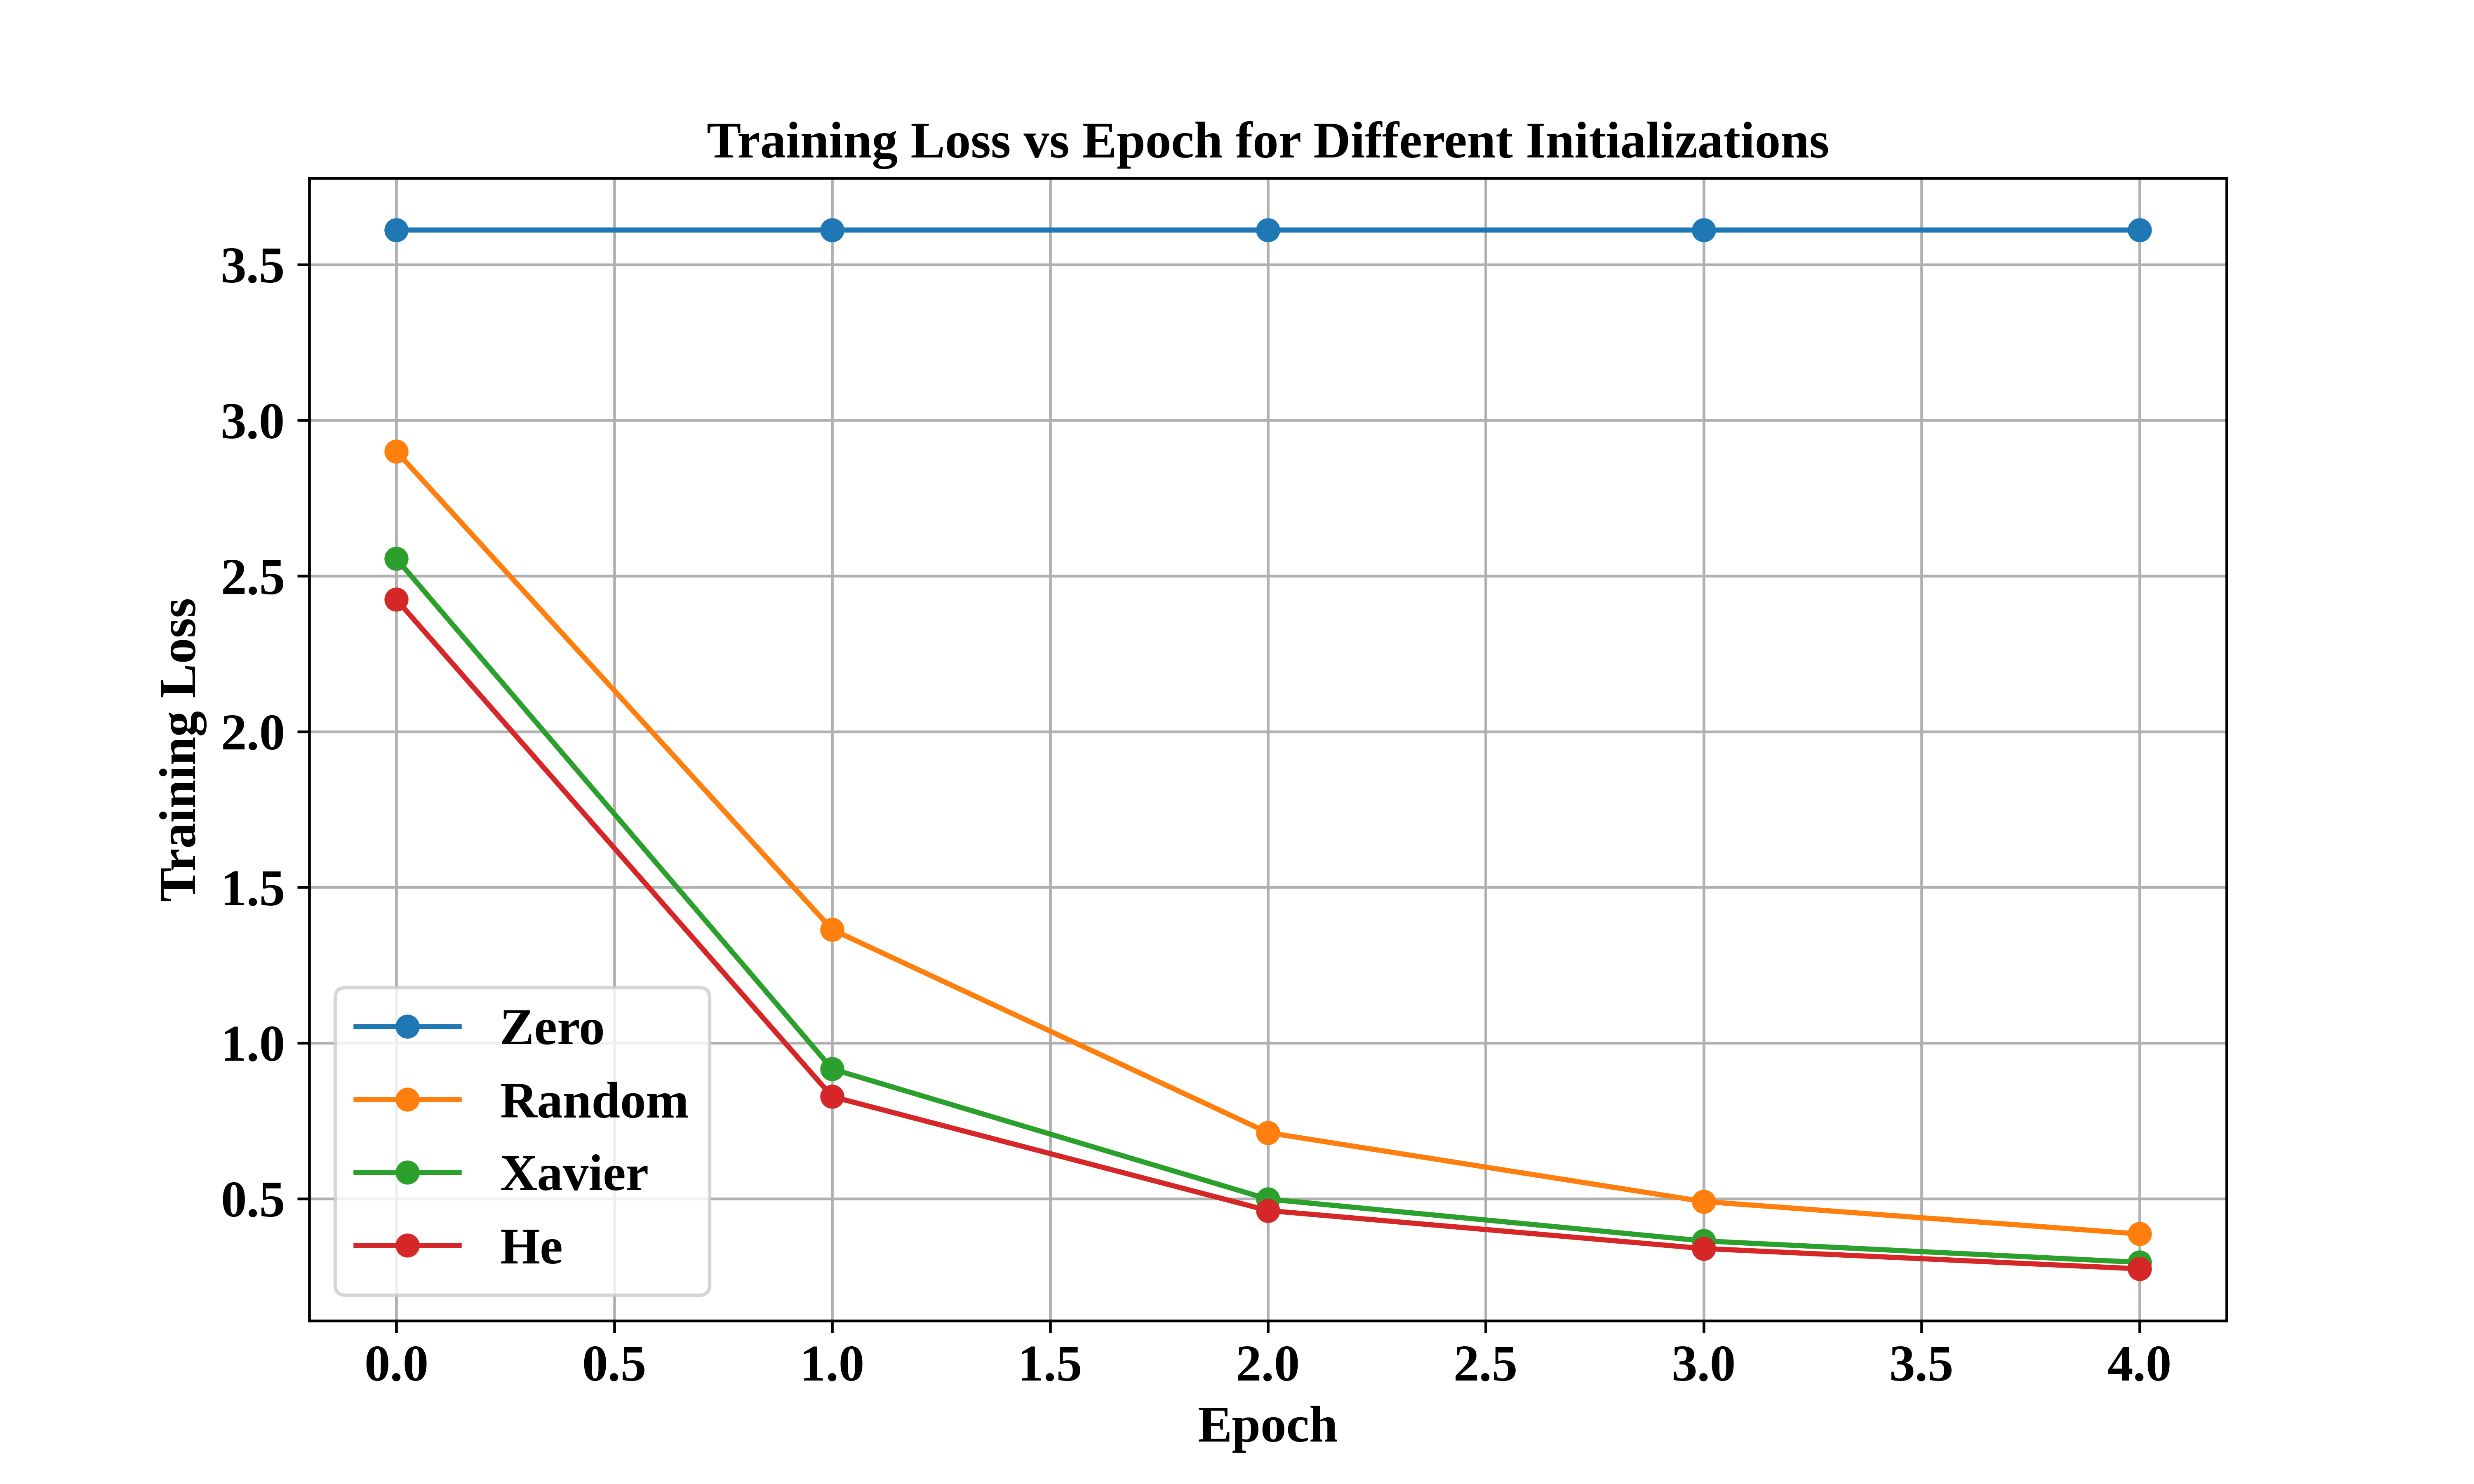
\includegraphics[width=0.8\textwidth]{Images/TrainingLossvsEpochforDifferentInitializations.png}
        \caption{Training Loss vs Epoch for Different Initializations}
        \label{fig:TrainingLossvsEpochforDifferentInitializations}
    \end{figure}
    \noindent\textbf{Inference:}\\
    The plot shows the training loss over 5 epochs for different weight initialization methods such as Zero, Random, Xavier, and He initialization.
    Random, Xavier, and He initialization show a steady decrease in training loss, while Zero initialization remains almost constant showing high loss of value approx. 3.6 .
    Proper weight initialization breaks symmetry and allows effective gradient-based learning, whereas zero initialization causes neurons to learn identical features and prevents effective training.

    \vspace{5 mm}

    \item\textbf{Weight Initialization: Validation Accuracy vs Epoch}
        \begin{figure}[H]
        \centering
        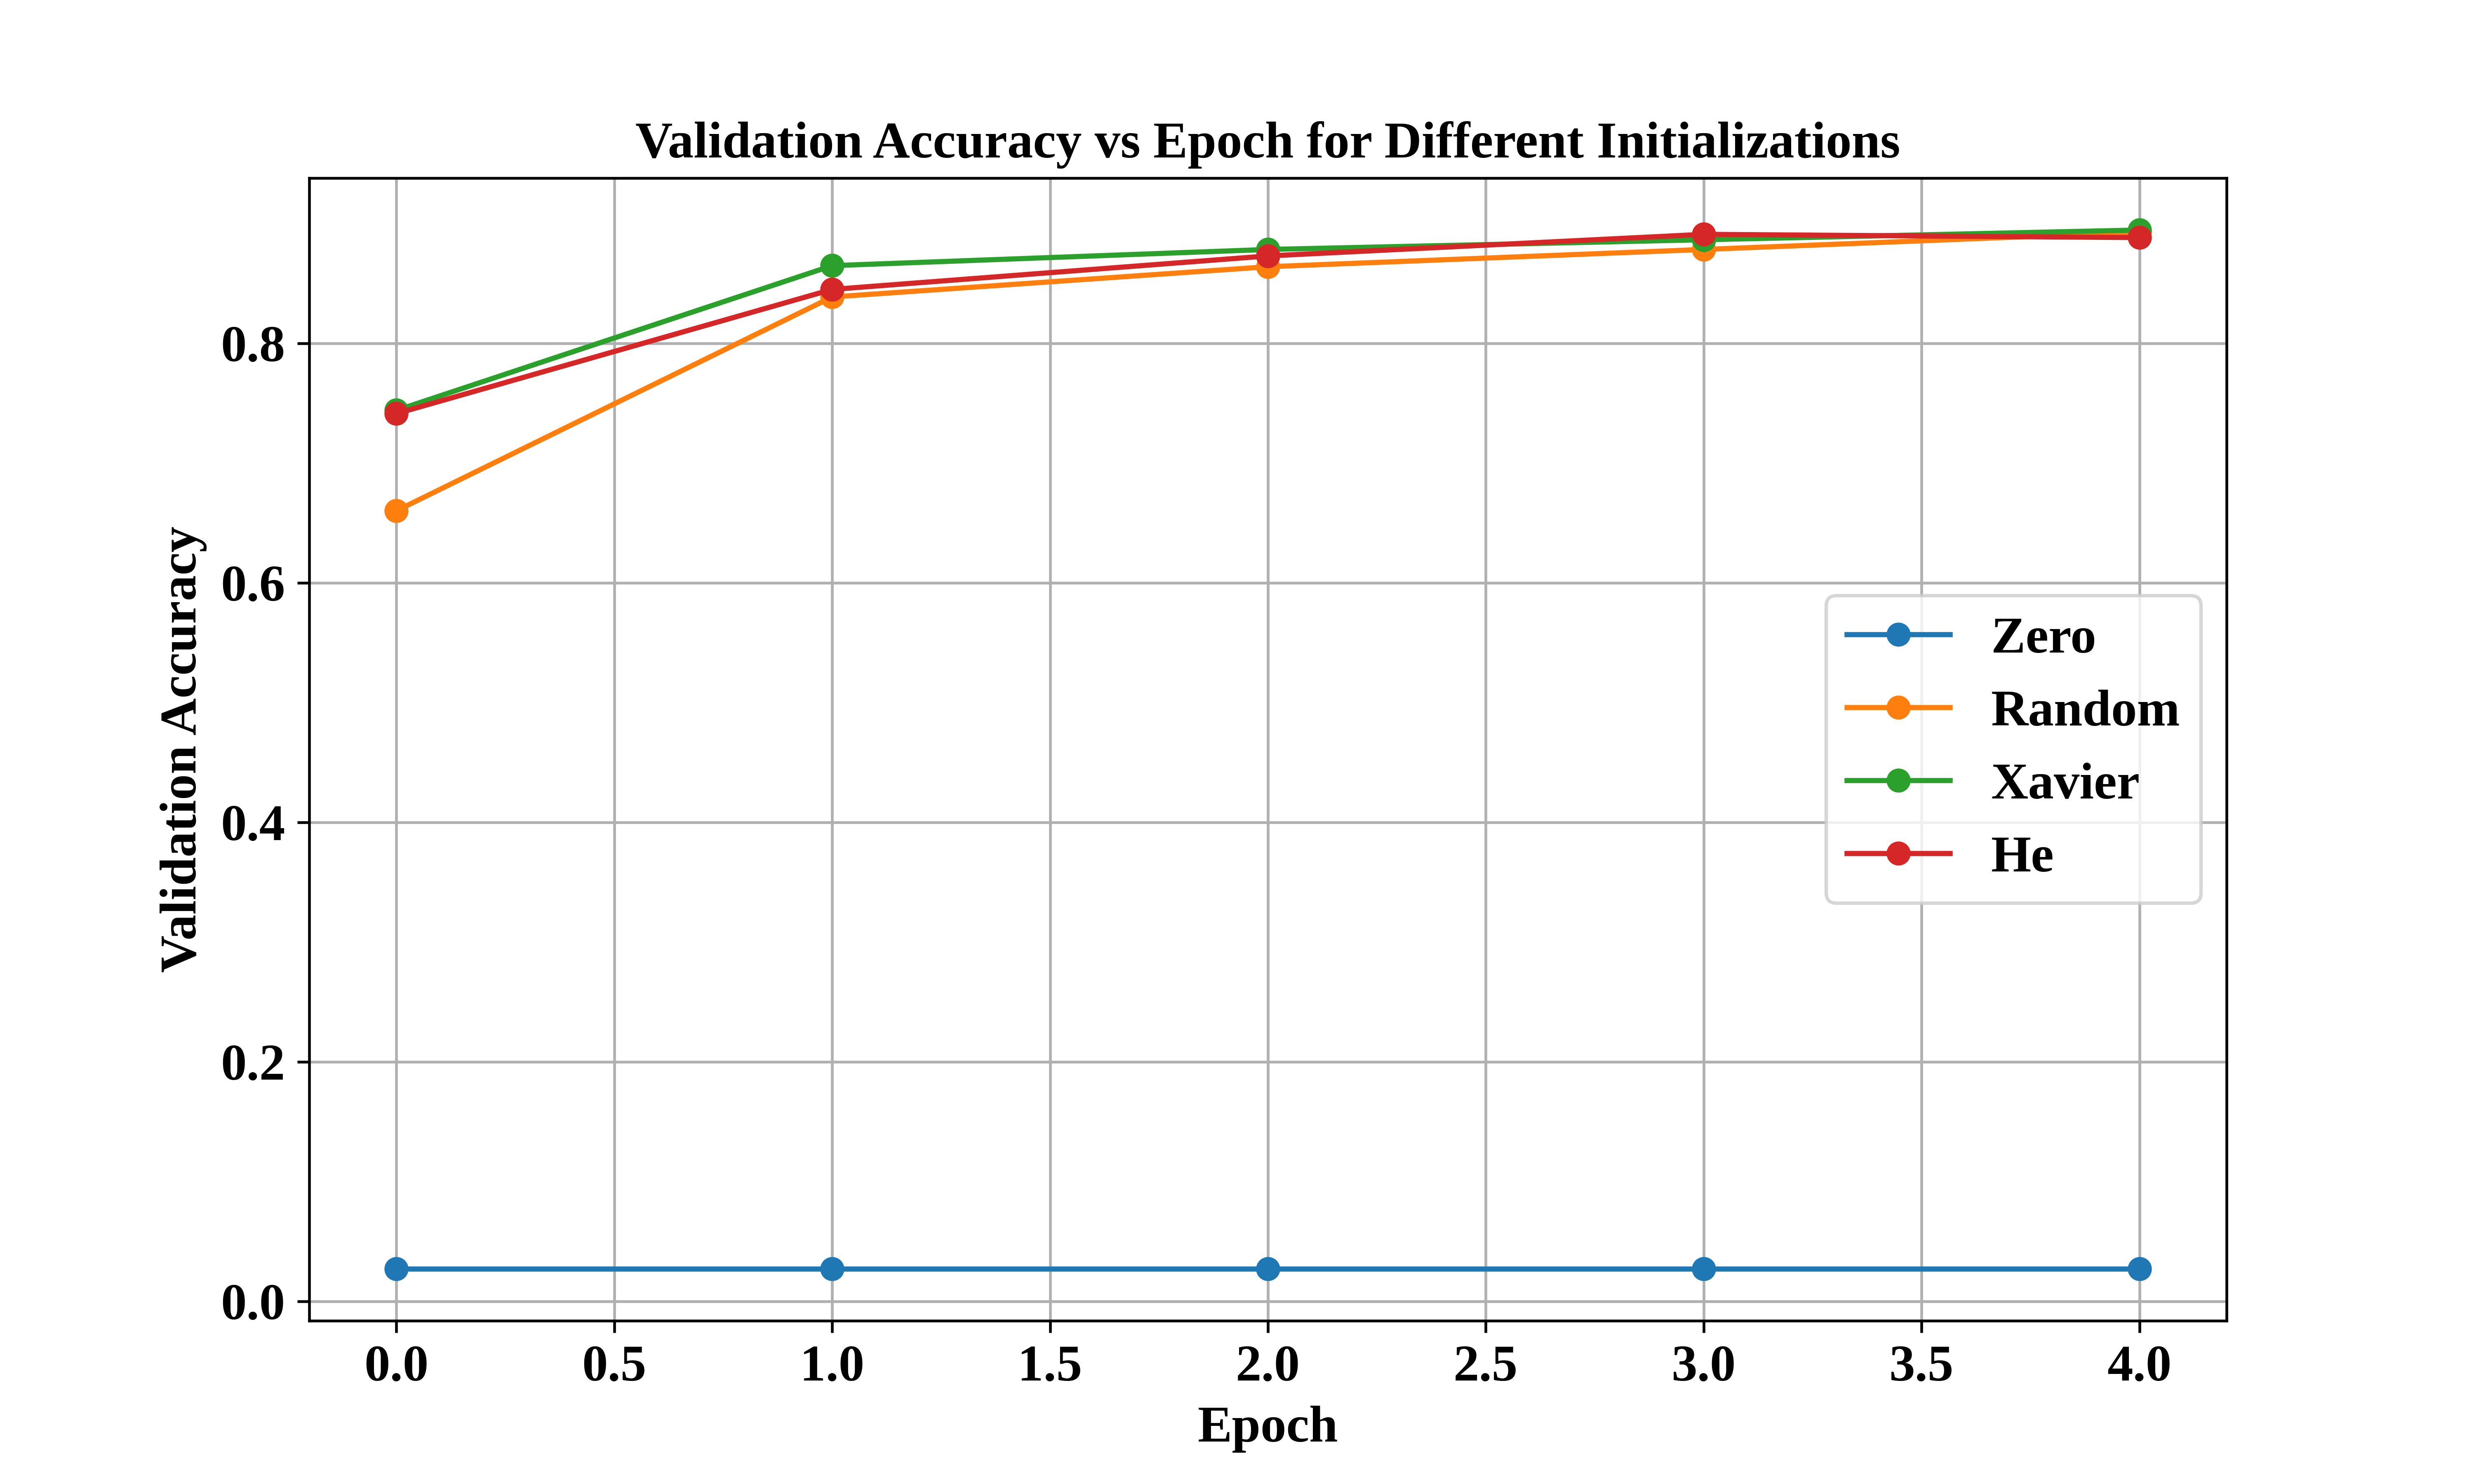
\includegraphics[width=0.8\textwidth]{Images/ValidationAccuracyvsEpochforDifferentInitializations.png}
        \caption{Validation Accuracy vs Epoch for Different Initializations}
        \label{fig:ValidationAccuracyvsEpochforDifferentInitializations}
    \end{figure}
    \noindent\textbf{Inference:}\\
    The plot shows the validation accuracy over 5 epochs for different weight initialization such as Zero, Random, Xavier, He.
    Xavier, He, and Random initializations rapidly increase in validation accuracy converging near 89 percent by epoch 5.
    Zero initialization fails to improve, remaining at validation accuracy of value approx. 0 percent across all epochs.
    Zero initialization causes weight symmetry, forcing all neurons to receive identical gradient updates and preventing feature learning.
    On the other hand, Xavier and He initialization break symmetry and prevent vanishing or exploding gradients, allowing effective optimization from epoch 0.

    \vspace{5mm}

    \item \textbf{No Regularization}

    \begin{figure}[H]
        \centering

        \begin{minipage}{0.48\textwidth}
            \centering
            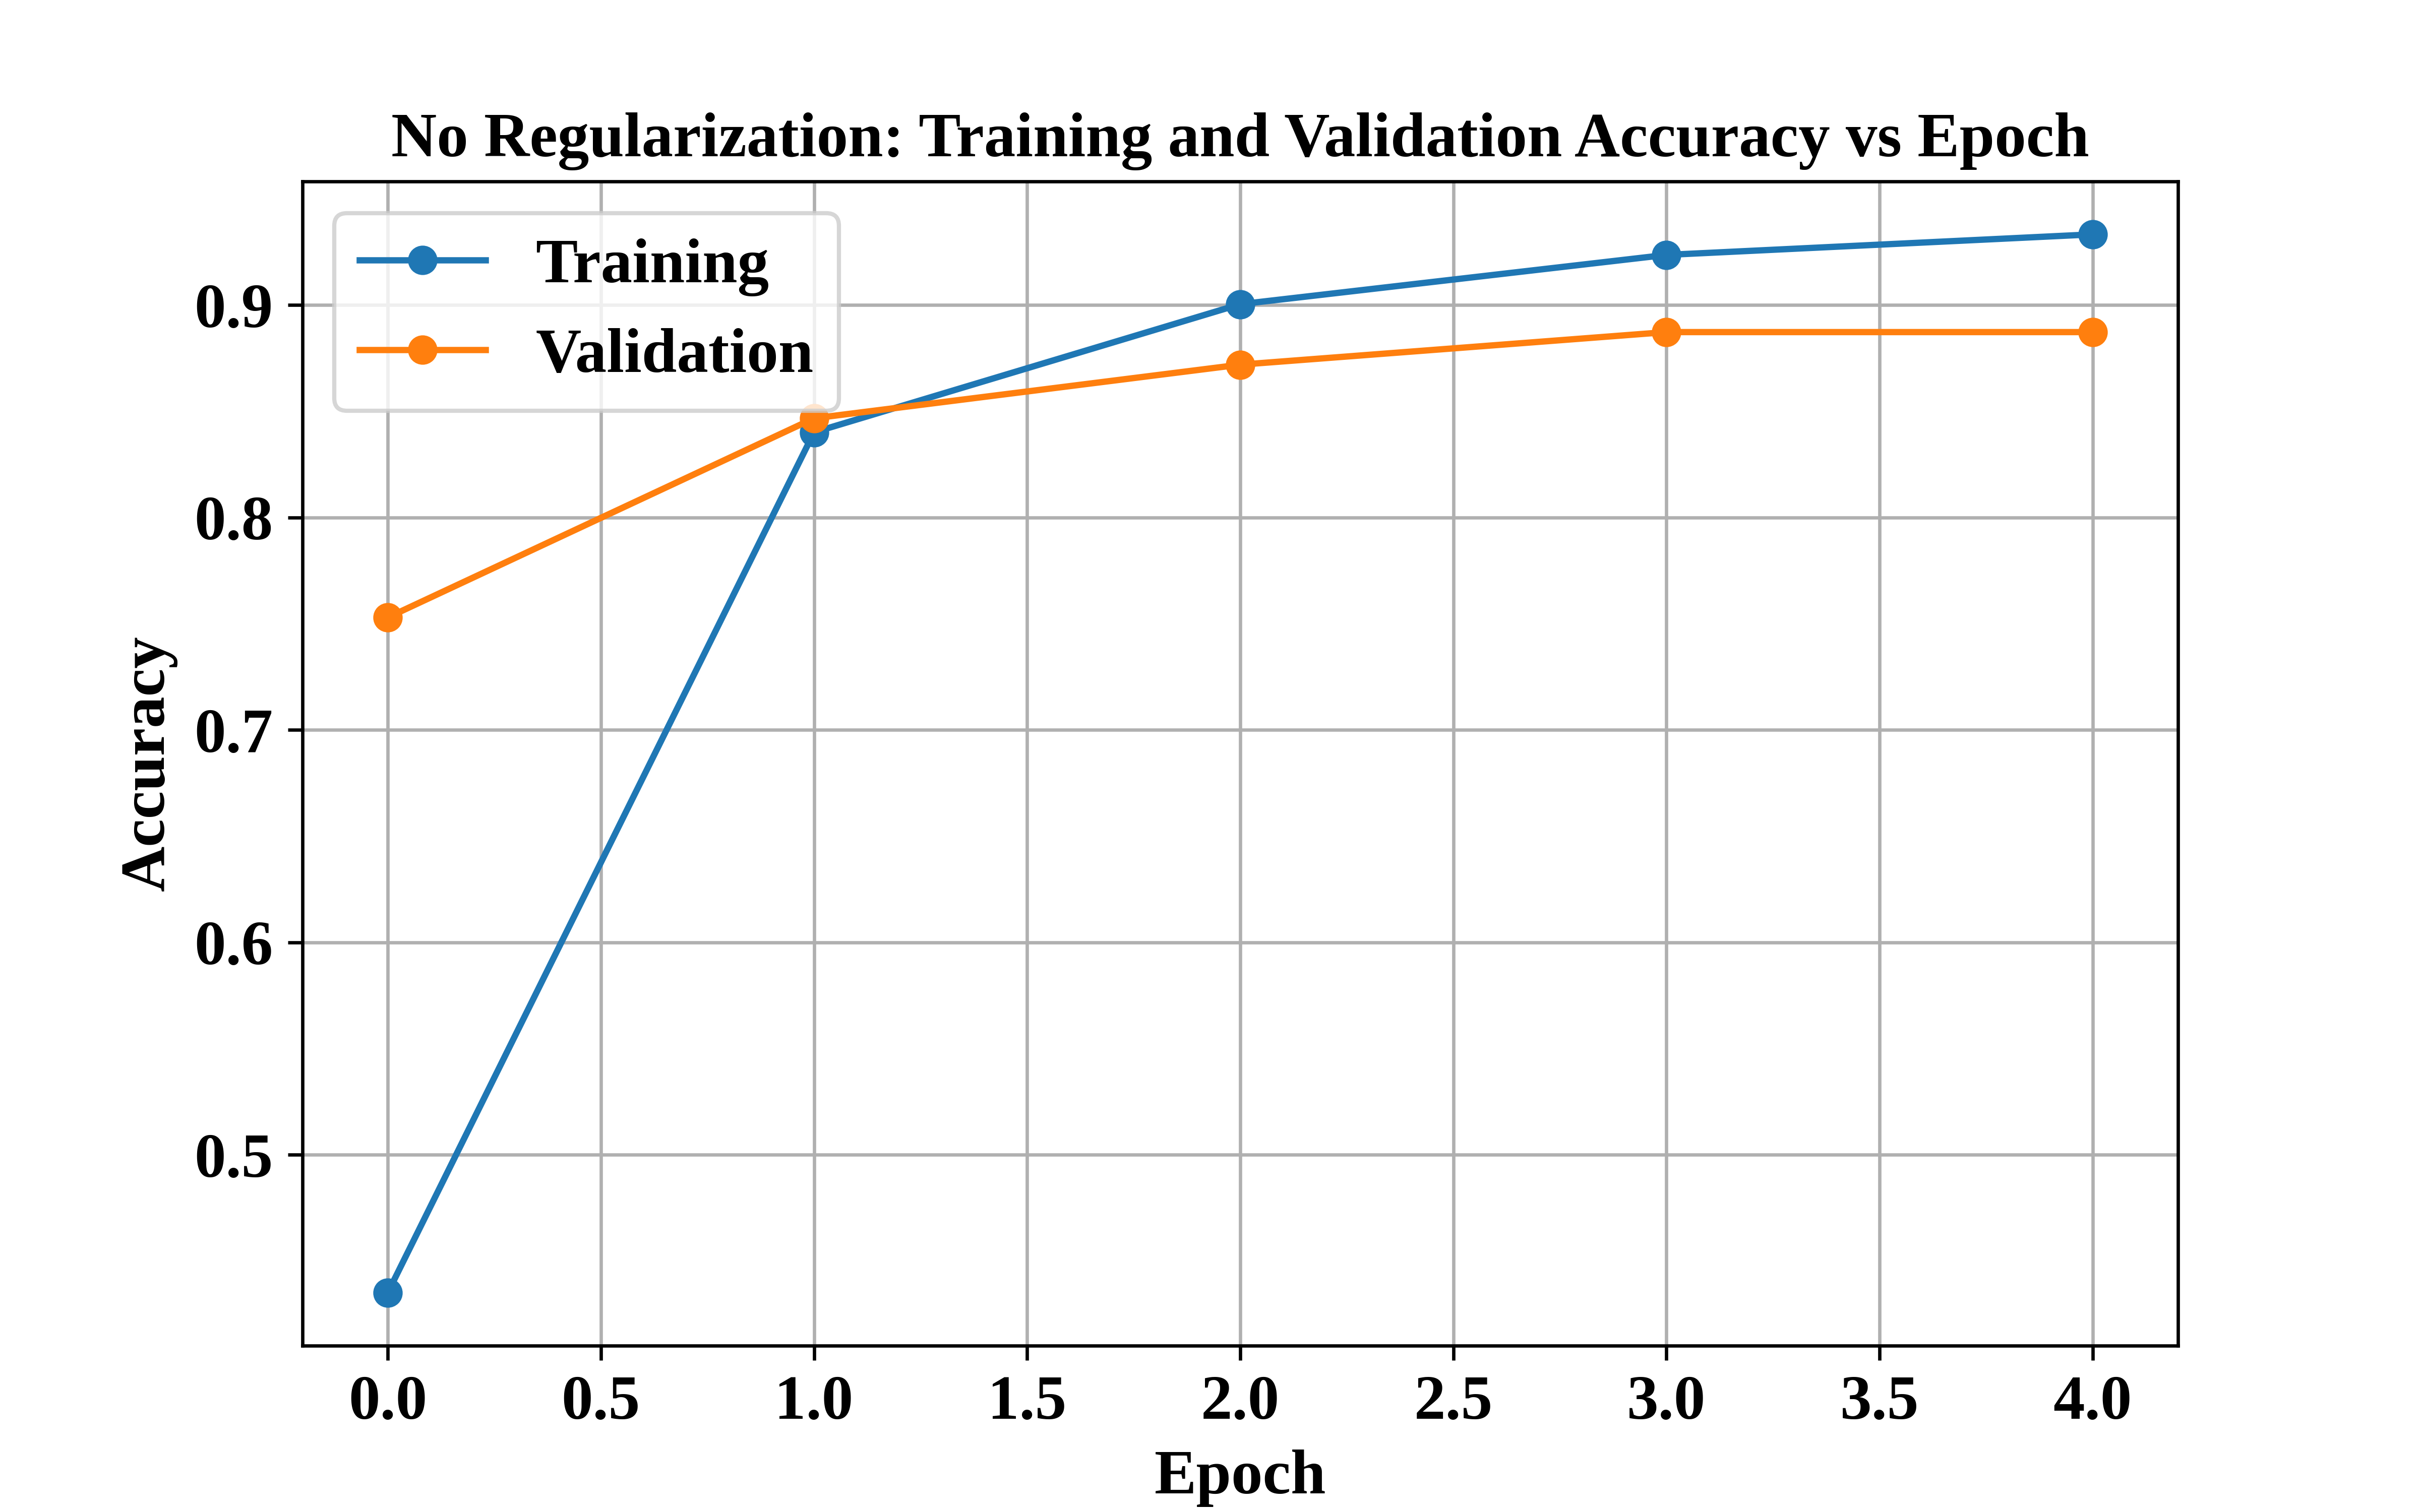
\includegraphics[width=1.0\textwidth]{Images/NoRegularization_TrainingandValidationAccuracyvsEpoch.png}
            \caption{Training and Validation Accuracy vs Epoch}
            \label{fig:AccuracyNoReg}
        \end{minipage}
        \hfill
        \begin{minipage}{0.48\textwidth}
            \centering
            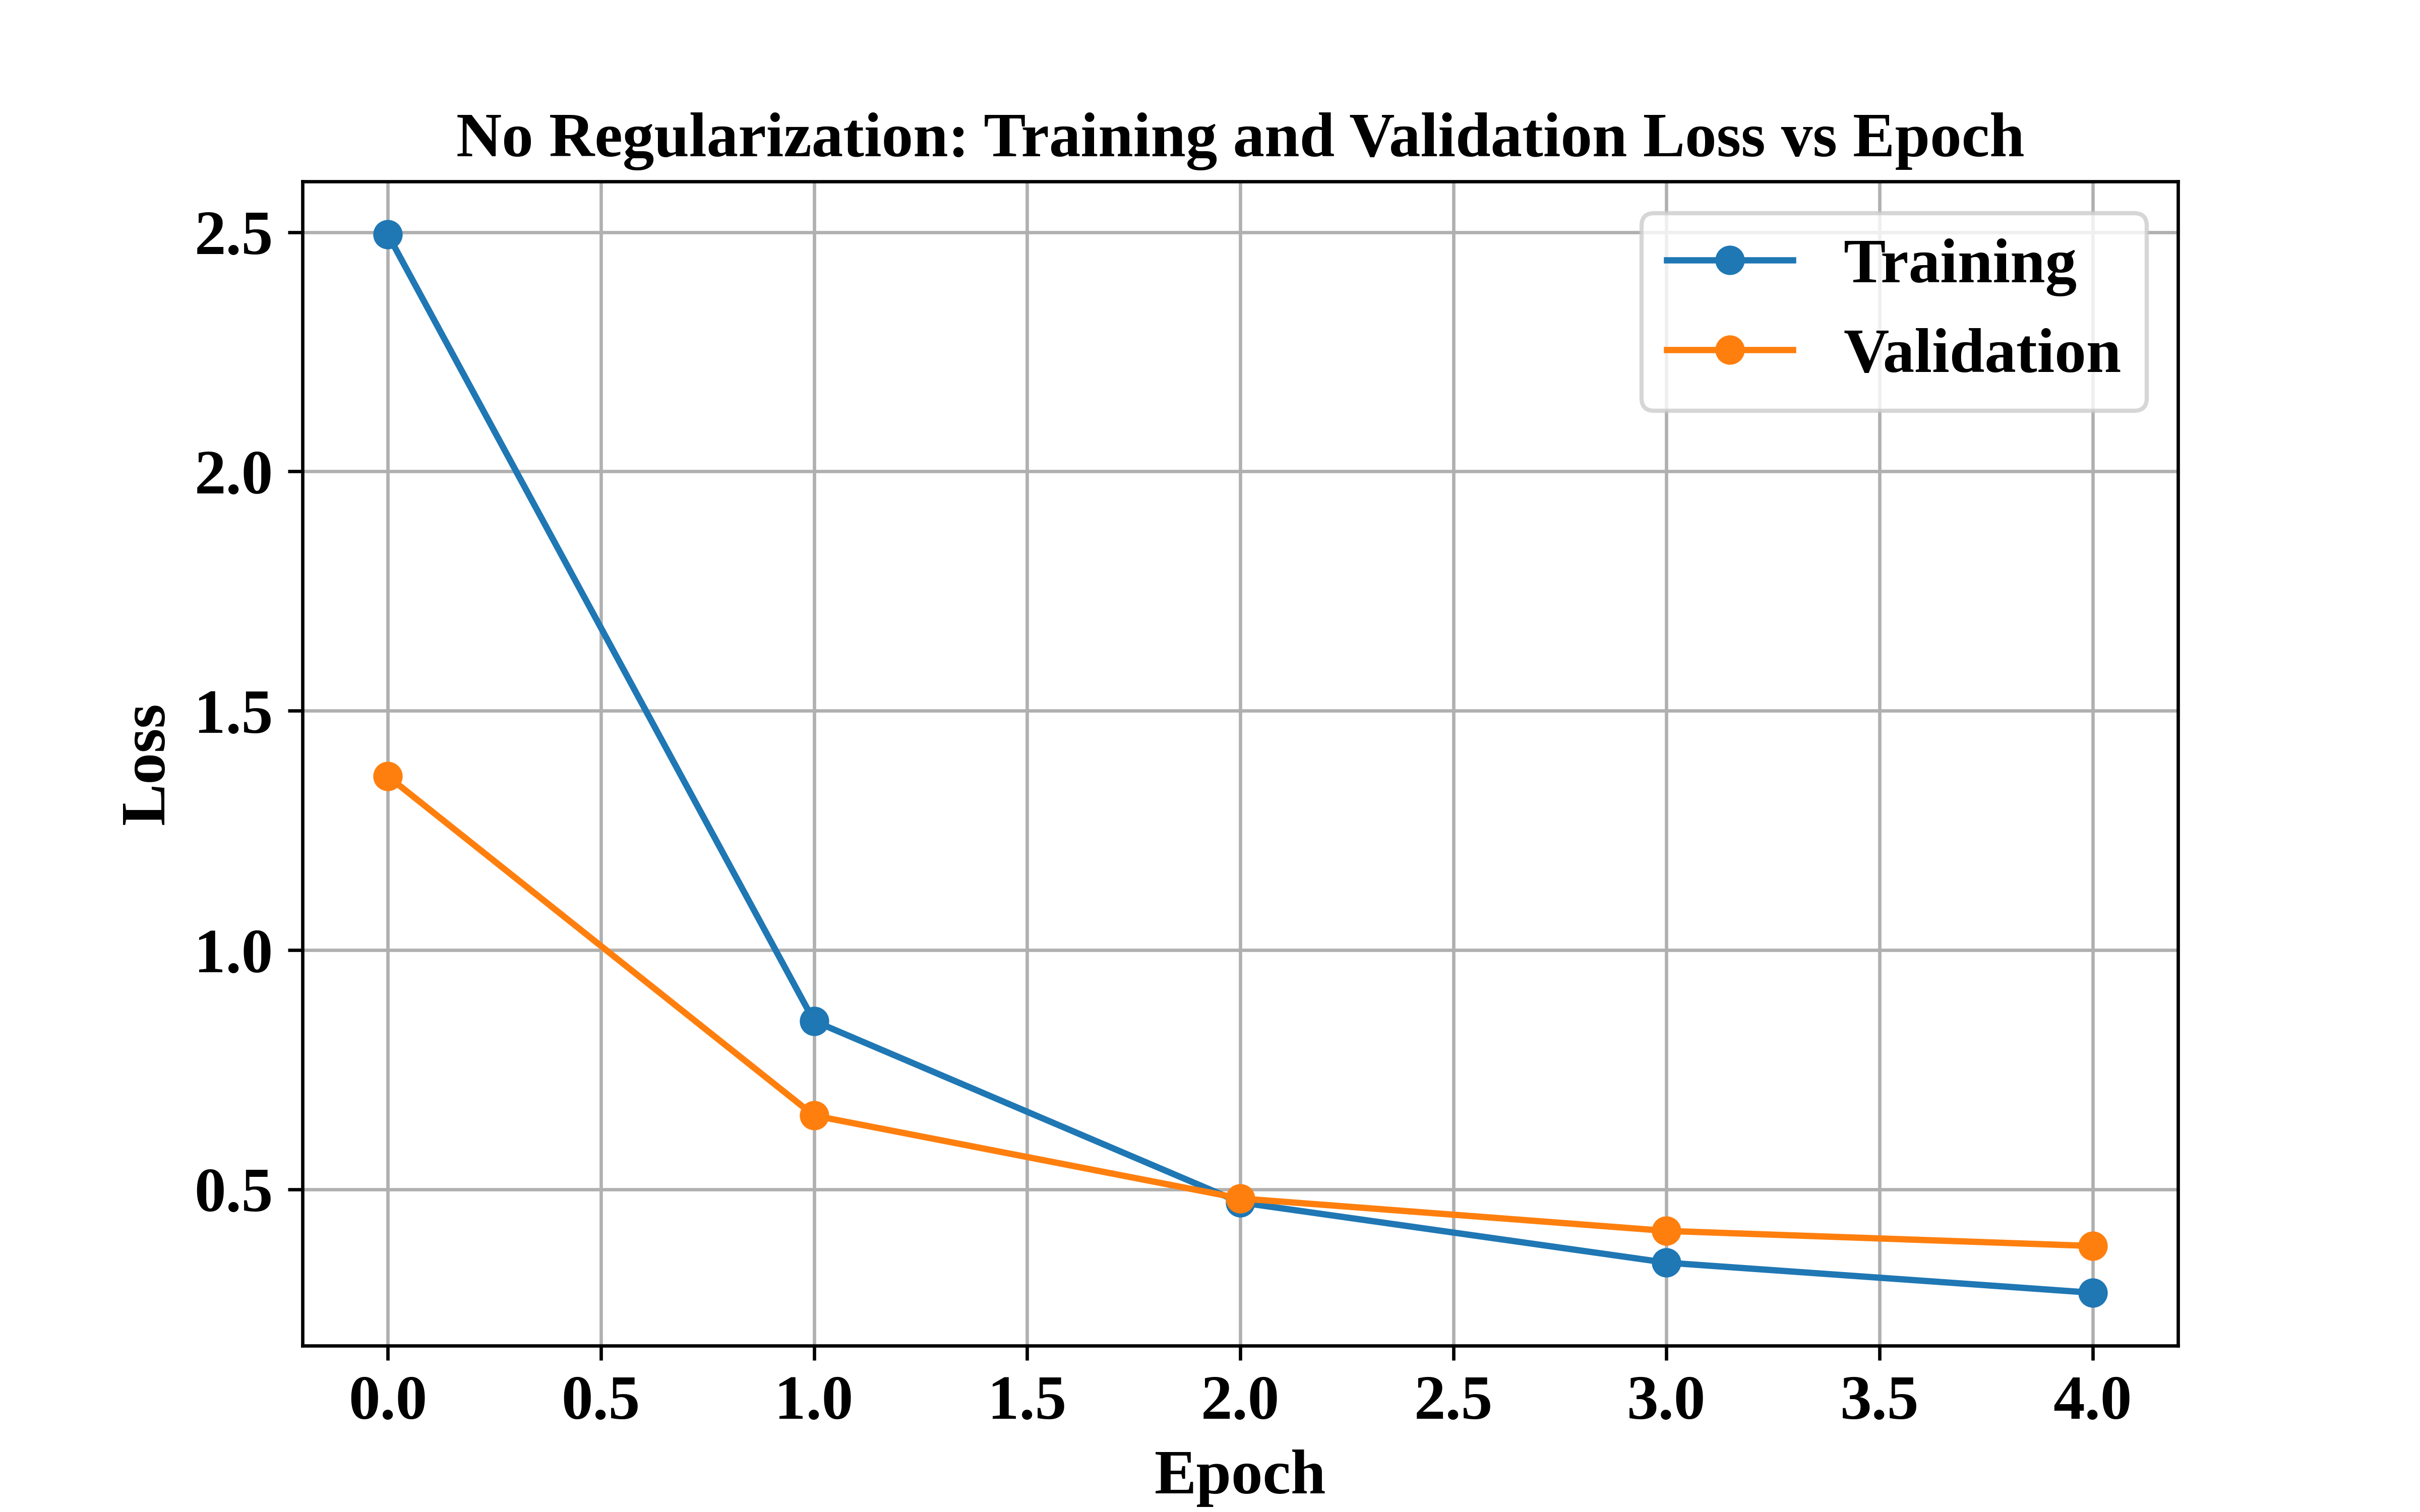
\includegraphics[width=1.0\textwidth]{Images/NoRegularization_TrainingandValidationLossvsEpoch.png}
            \caption{Training and Validation Loss vs Epoch}
            \label{fig:LossNoReg}
        \end{minipage}

    \end{figure}
    \noindent\textbf{Training and Validation Accuracy vs Epoch Inference:}\\
    The plot compares training accuracy and validation accuracy across 5 epochs for models trained with no regularization.
    The validation accuracy shows stable increase whereas training accuracy increases sharply then stabilises.

    \vspace{5mm}
    \noindent\textbf{Training and Validation Loss vs Epoch Inference:}\\
    The plot compares training  and validation loss across 5 epochs for models trained with no regularization.
    Both the curves shows steady decrease and reaches minimum of approx. 0.5 loss value.

    \vspace{5mm}

    \item \textbf{L2 Regularization}

    \begin{figure}[H]
        \centering

        \begin{minipage}{0.48\textwidth}
            \centering
            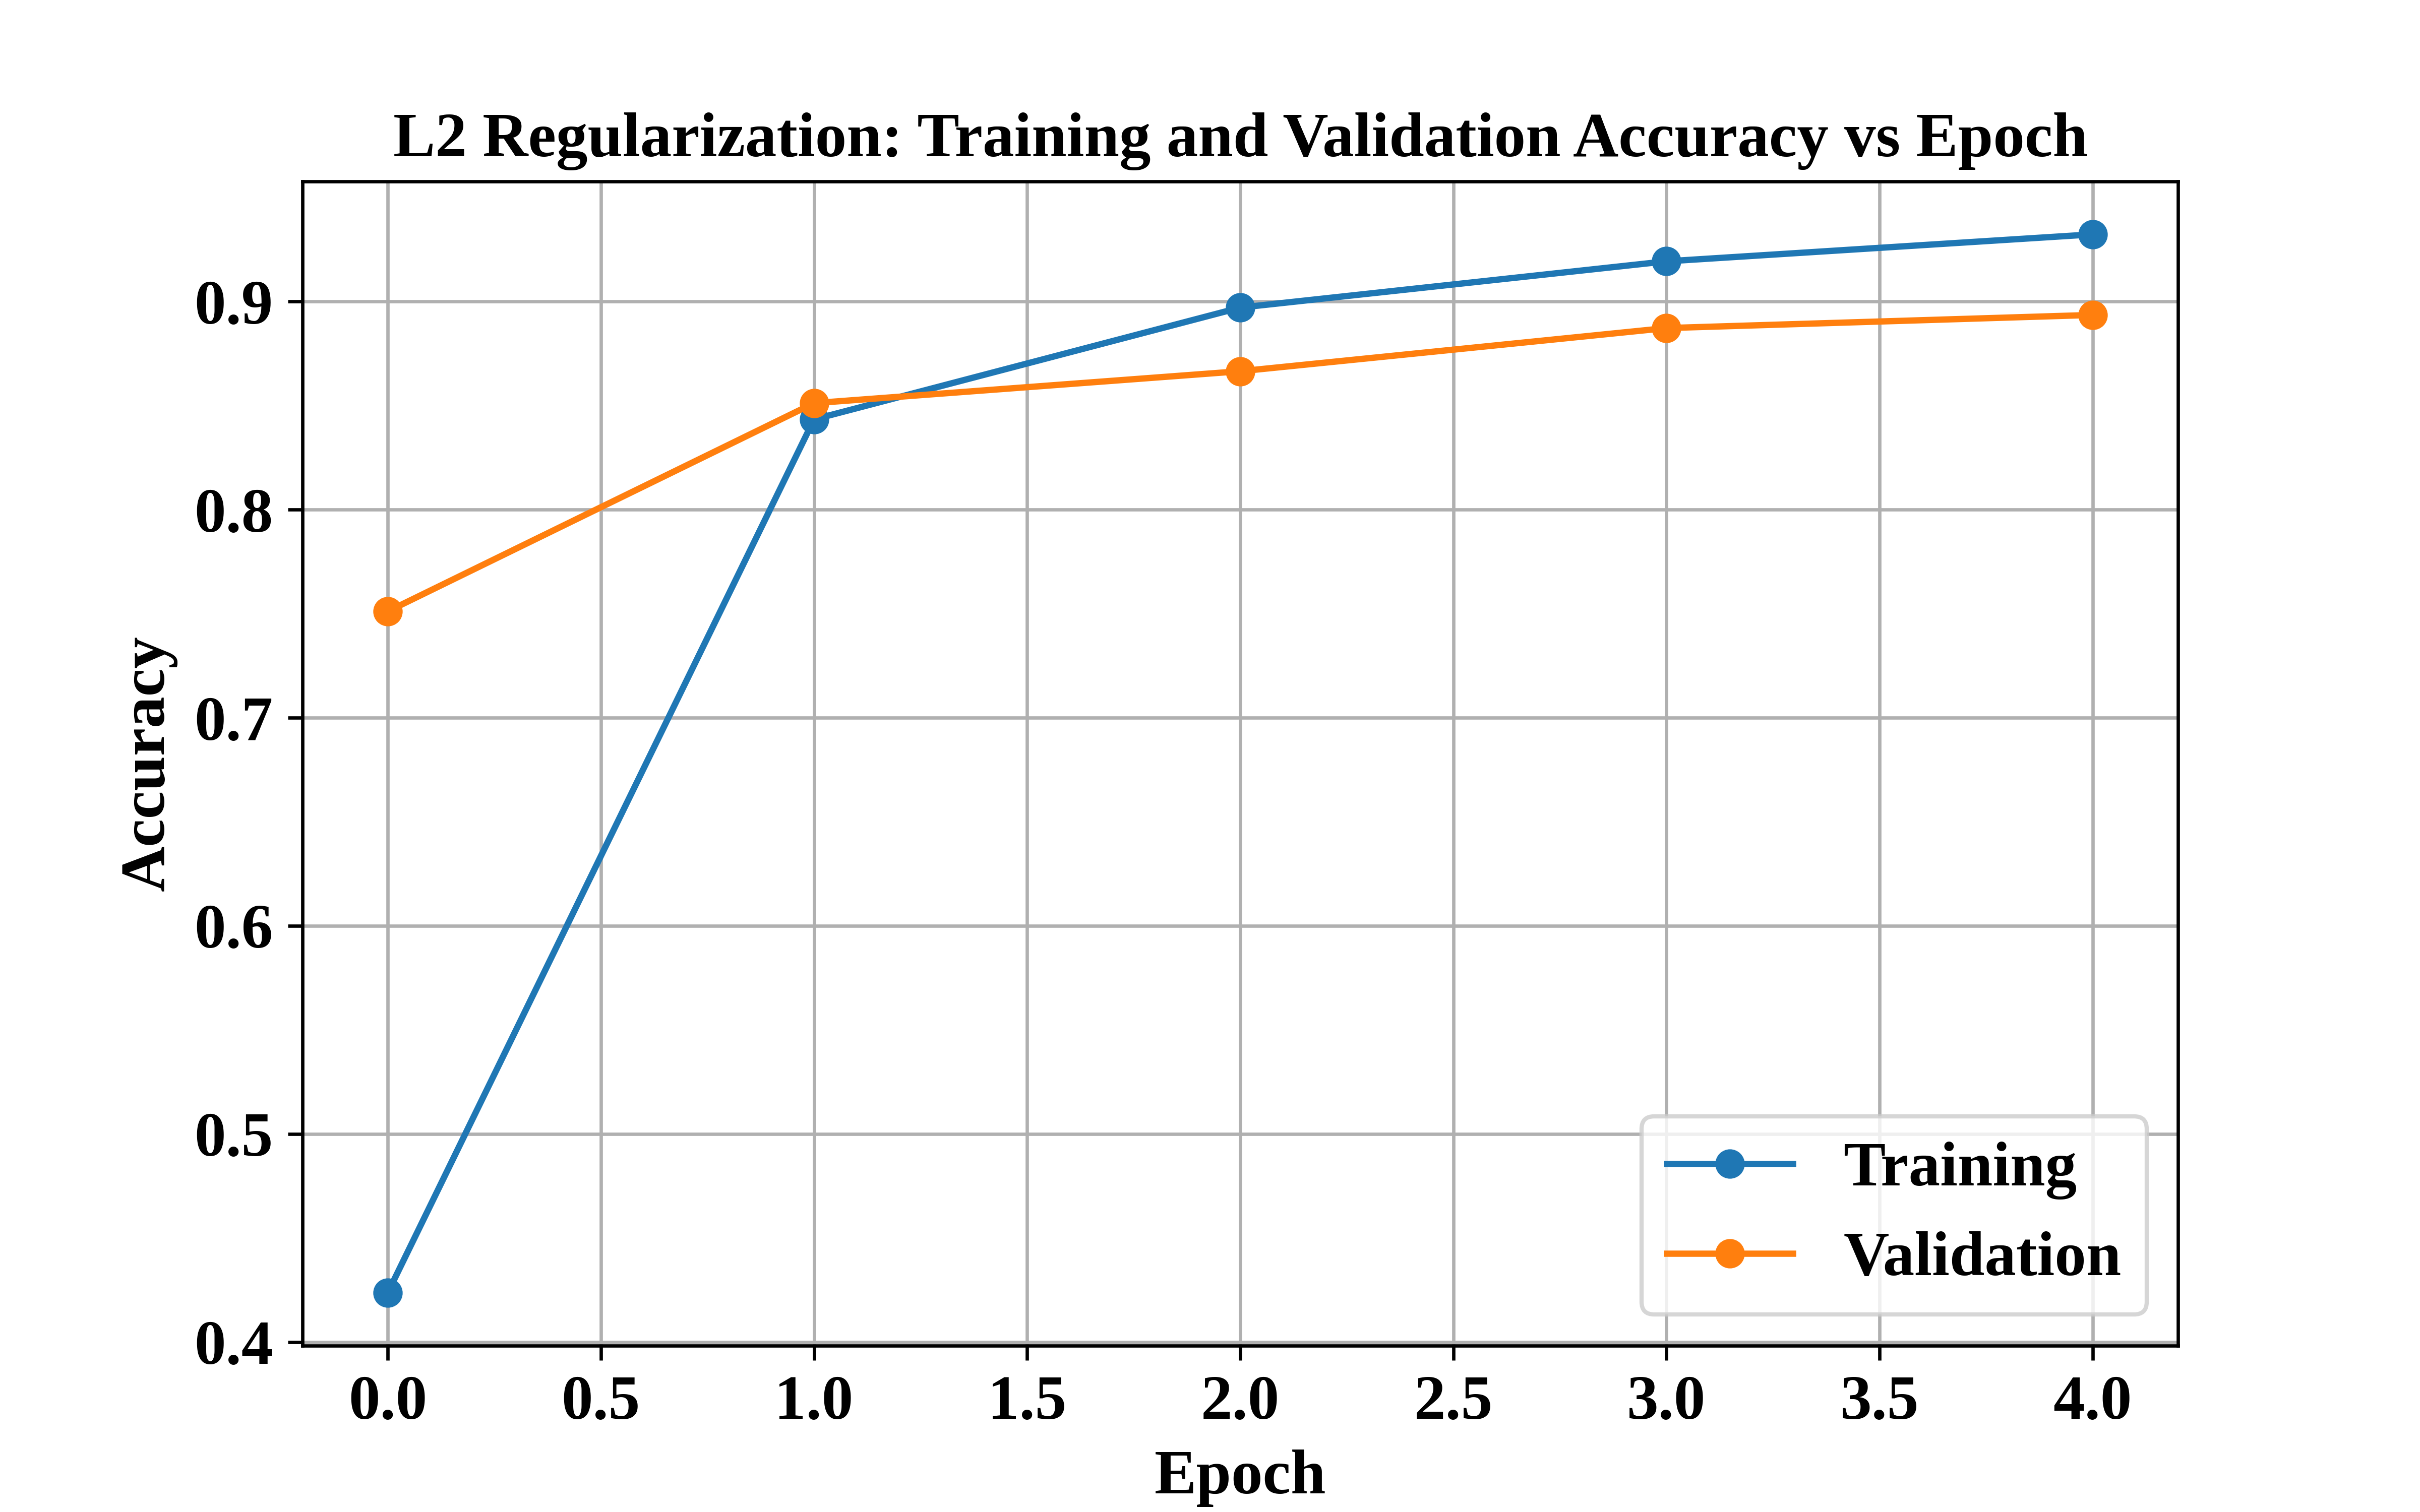
\includegraphics[width=1.0\textwidth]{Images/L2Regularization_TrainingandValidationAccuracyvsEpoch.png}
            \caption{Training and Validation Accuracy vs Epoch}
            \label{fig:AccuracyL2}
        \end{minipage}
        \hfill
        \begin{minipage}{0.48\textwidth}
            \centering
            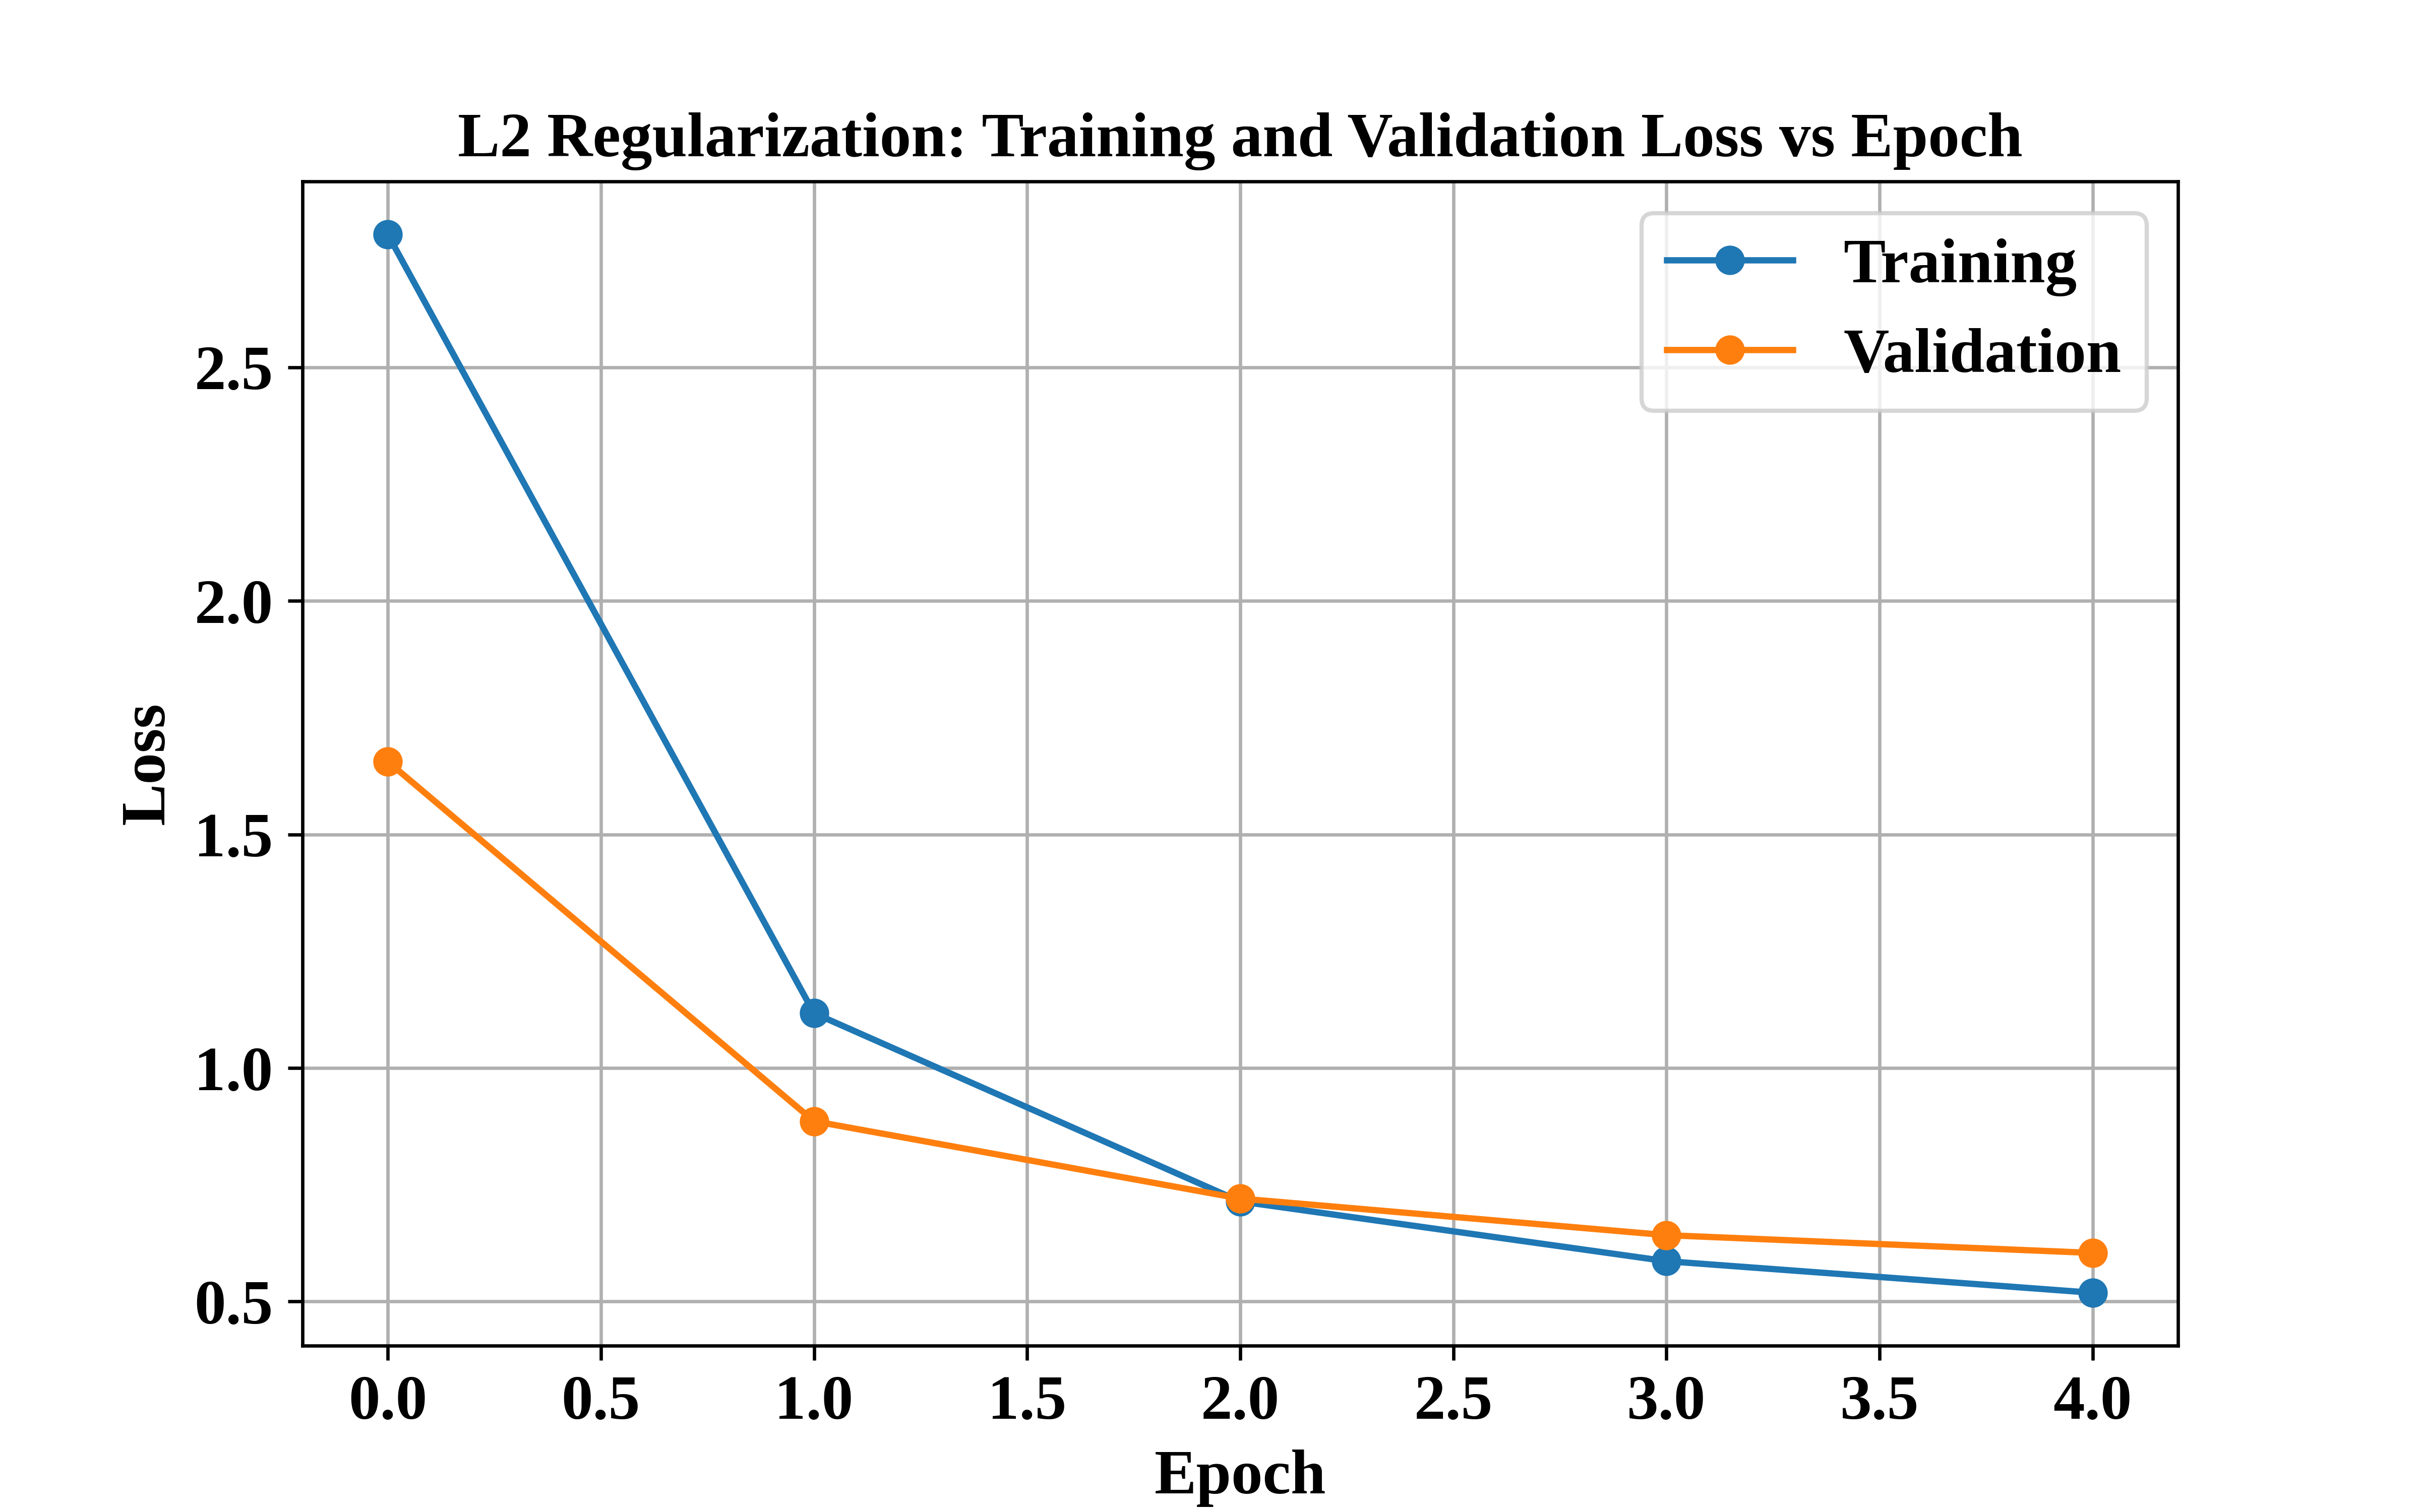
\includegraphics[width=1.0\textwidth]{Images/L2Regularization_TrainingandValidationLossvsEpoch.png}
            \caption{Training and Validation Loss vs Epoch}
            \label{fig:LossL2}
        \end{minipage}

    \end{figure}

    \vspace{5mm}

    \noindent\textbf{Training and Validation Accuracy vs Epoch Inference:}\\
    The plot compares training accuracy and validation accuracy across 5 epochs for models trained with L2 regularization.
    The validation accuracy shows stable increase whereas training accuracy increases sharply then stabilises.

    \vspace{5mm}
    \noindent\textbf{Training and Validation Loss vs Epoch Inference:}\\
    The plot compares training and validation loss across 5 epochs for models trained with L2 regularization.
    Both the curves shows steady decrease and reaches minimum of approx. 0.5 loss value.

    \clearpage
    \item \textbf{Dropout}

    \begin{figure}[H]
        \centering

        \begin{minipage}{0.48\textwidth}
            \centering
            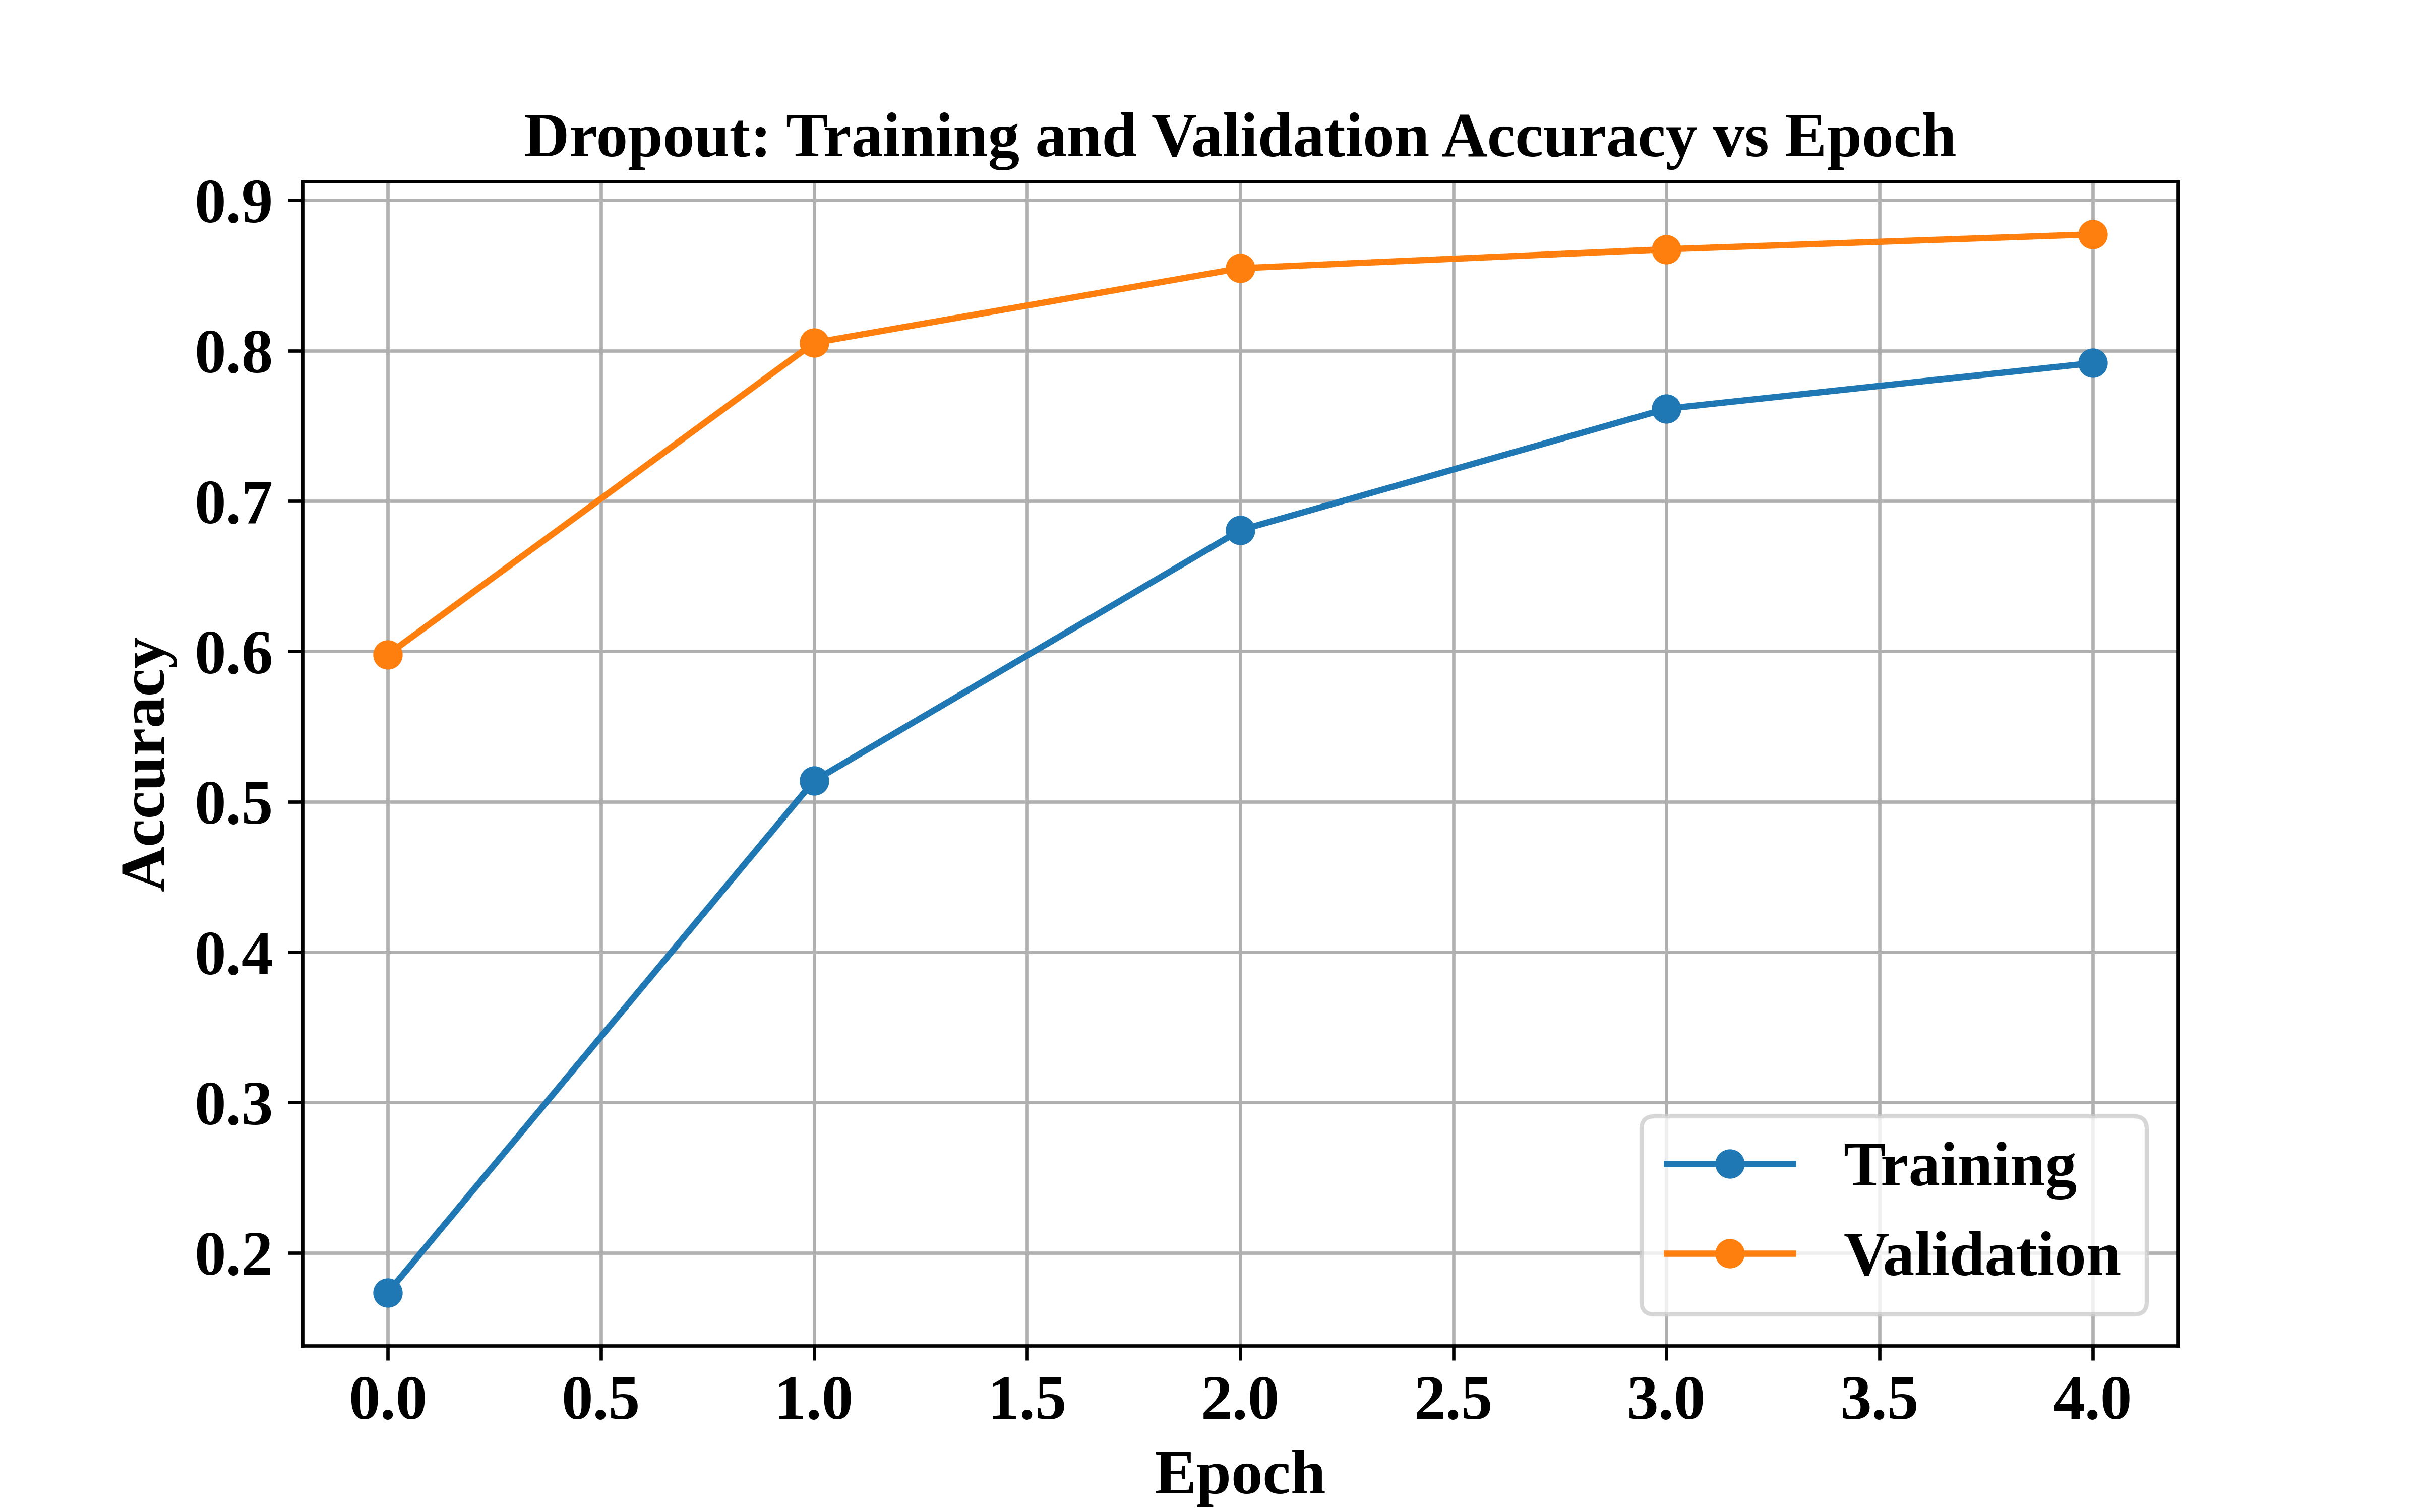
\includegraphics[width=1.0\textwidth]{Images/Dropout_TrainingandValidationAccuracyvsEpoch.png}
            \caption{Training and Validation Accuracy vs Epoch}
            \label{fig:AccuracyDropout}
        \end{minipage}
        \hfill
        \begin{minipage}{0.48\textwidth}
            \centering
            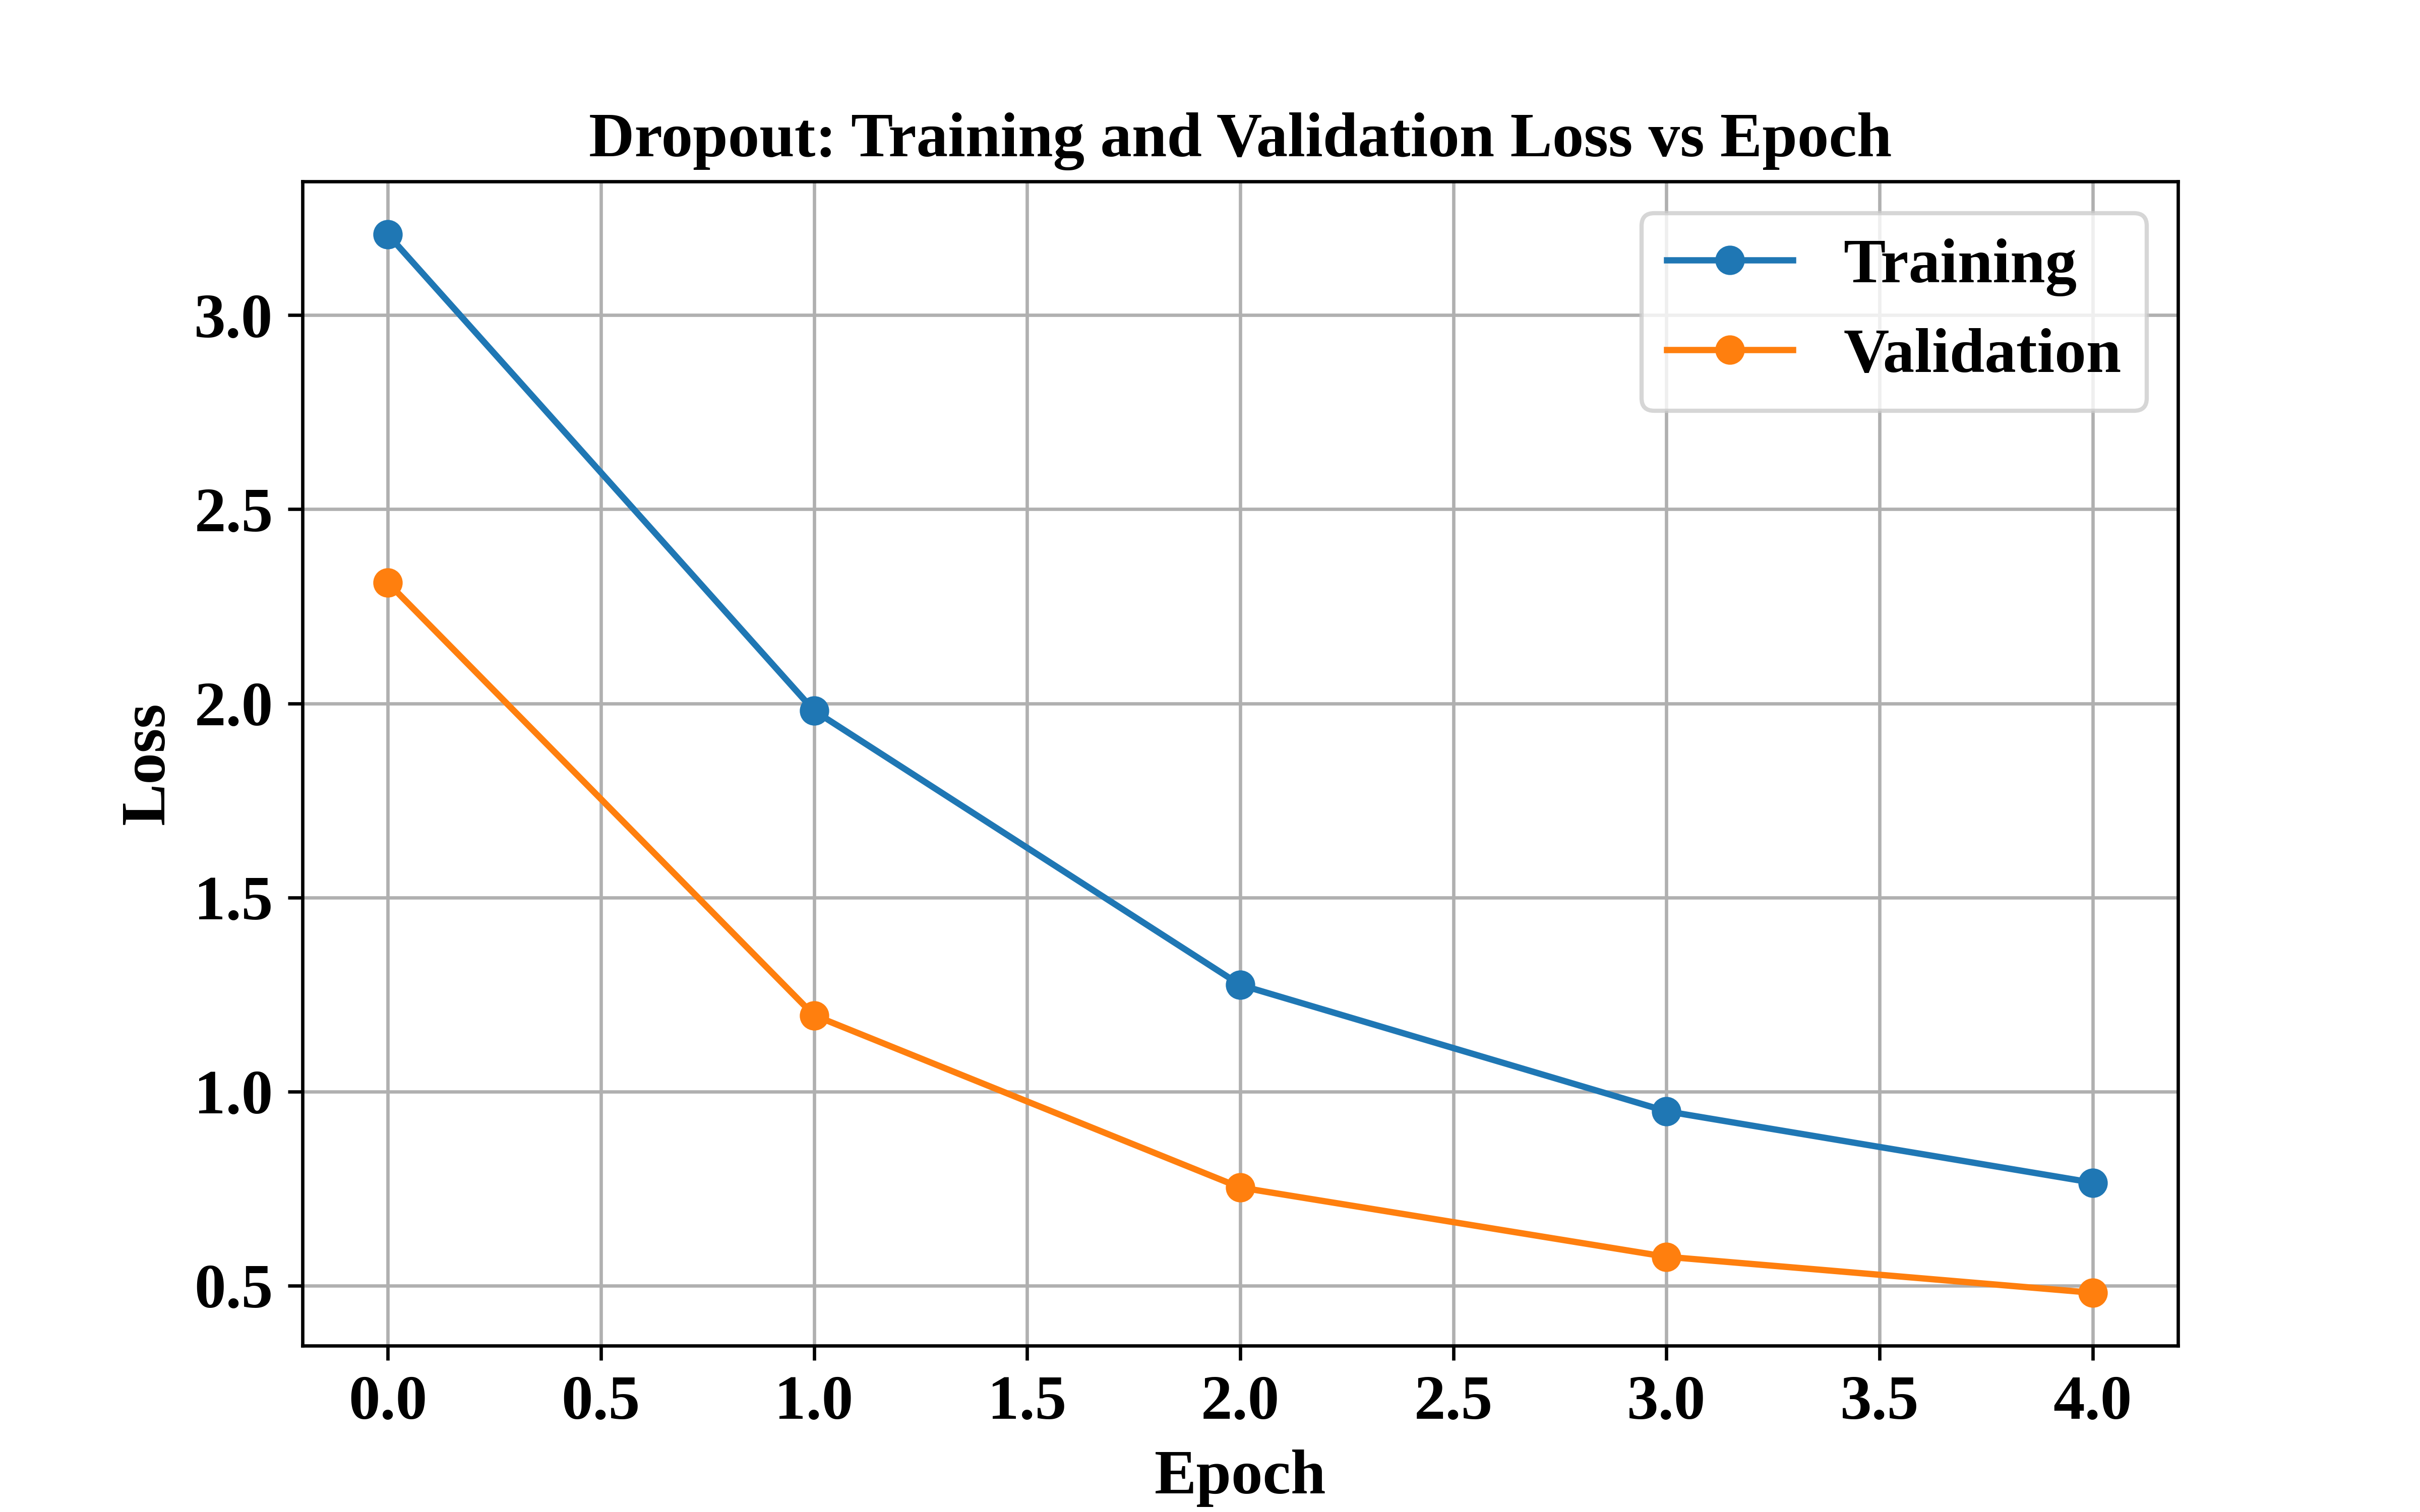
\includegraphics[width=1.0\textwidth]{Images/Dropout_TrainingandValidationLossvsEpoch.png}
            \caption{Training and Validation Loss vs Epoch}
            \label{fig:LossDropout}
        \end{minipage}

    \end{figure}
    \noindent\textbf{Training and Validation Accuracy vs Epoch Inference:}\\
    The plot compares training and validation accuracy across 5 epochs for models trained with dropout.
    Both the curves shows steady increase with validation curve having higher accuracy consistently.

    \vspace{5mm}
    \noindent\textbf{Training and Validation Loss vs Epoch Inference:}\\
    The plot compares training and validation loss across 5 epochs for models trained with dropout.
    Both the curves shows steady decrease with validation curve having lower loss consistently.

    \vspace{5mm}
    \item \textbf{Batch Normalization}

    \begin{figure}[H]
        \centering

        \begin{minipage}{0.48\textwidth}
            \centering
            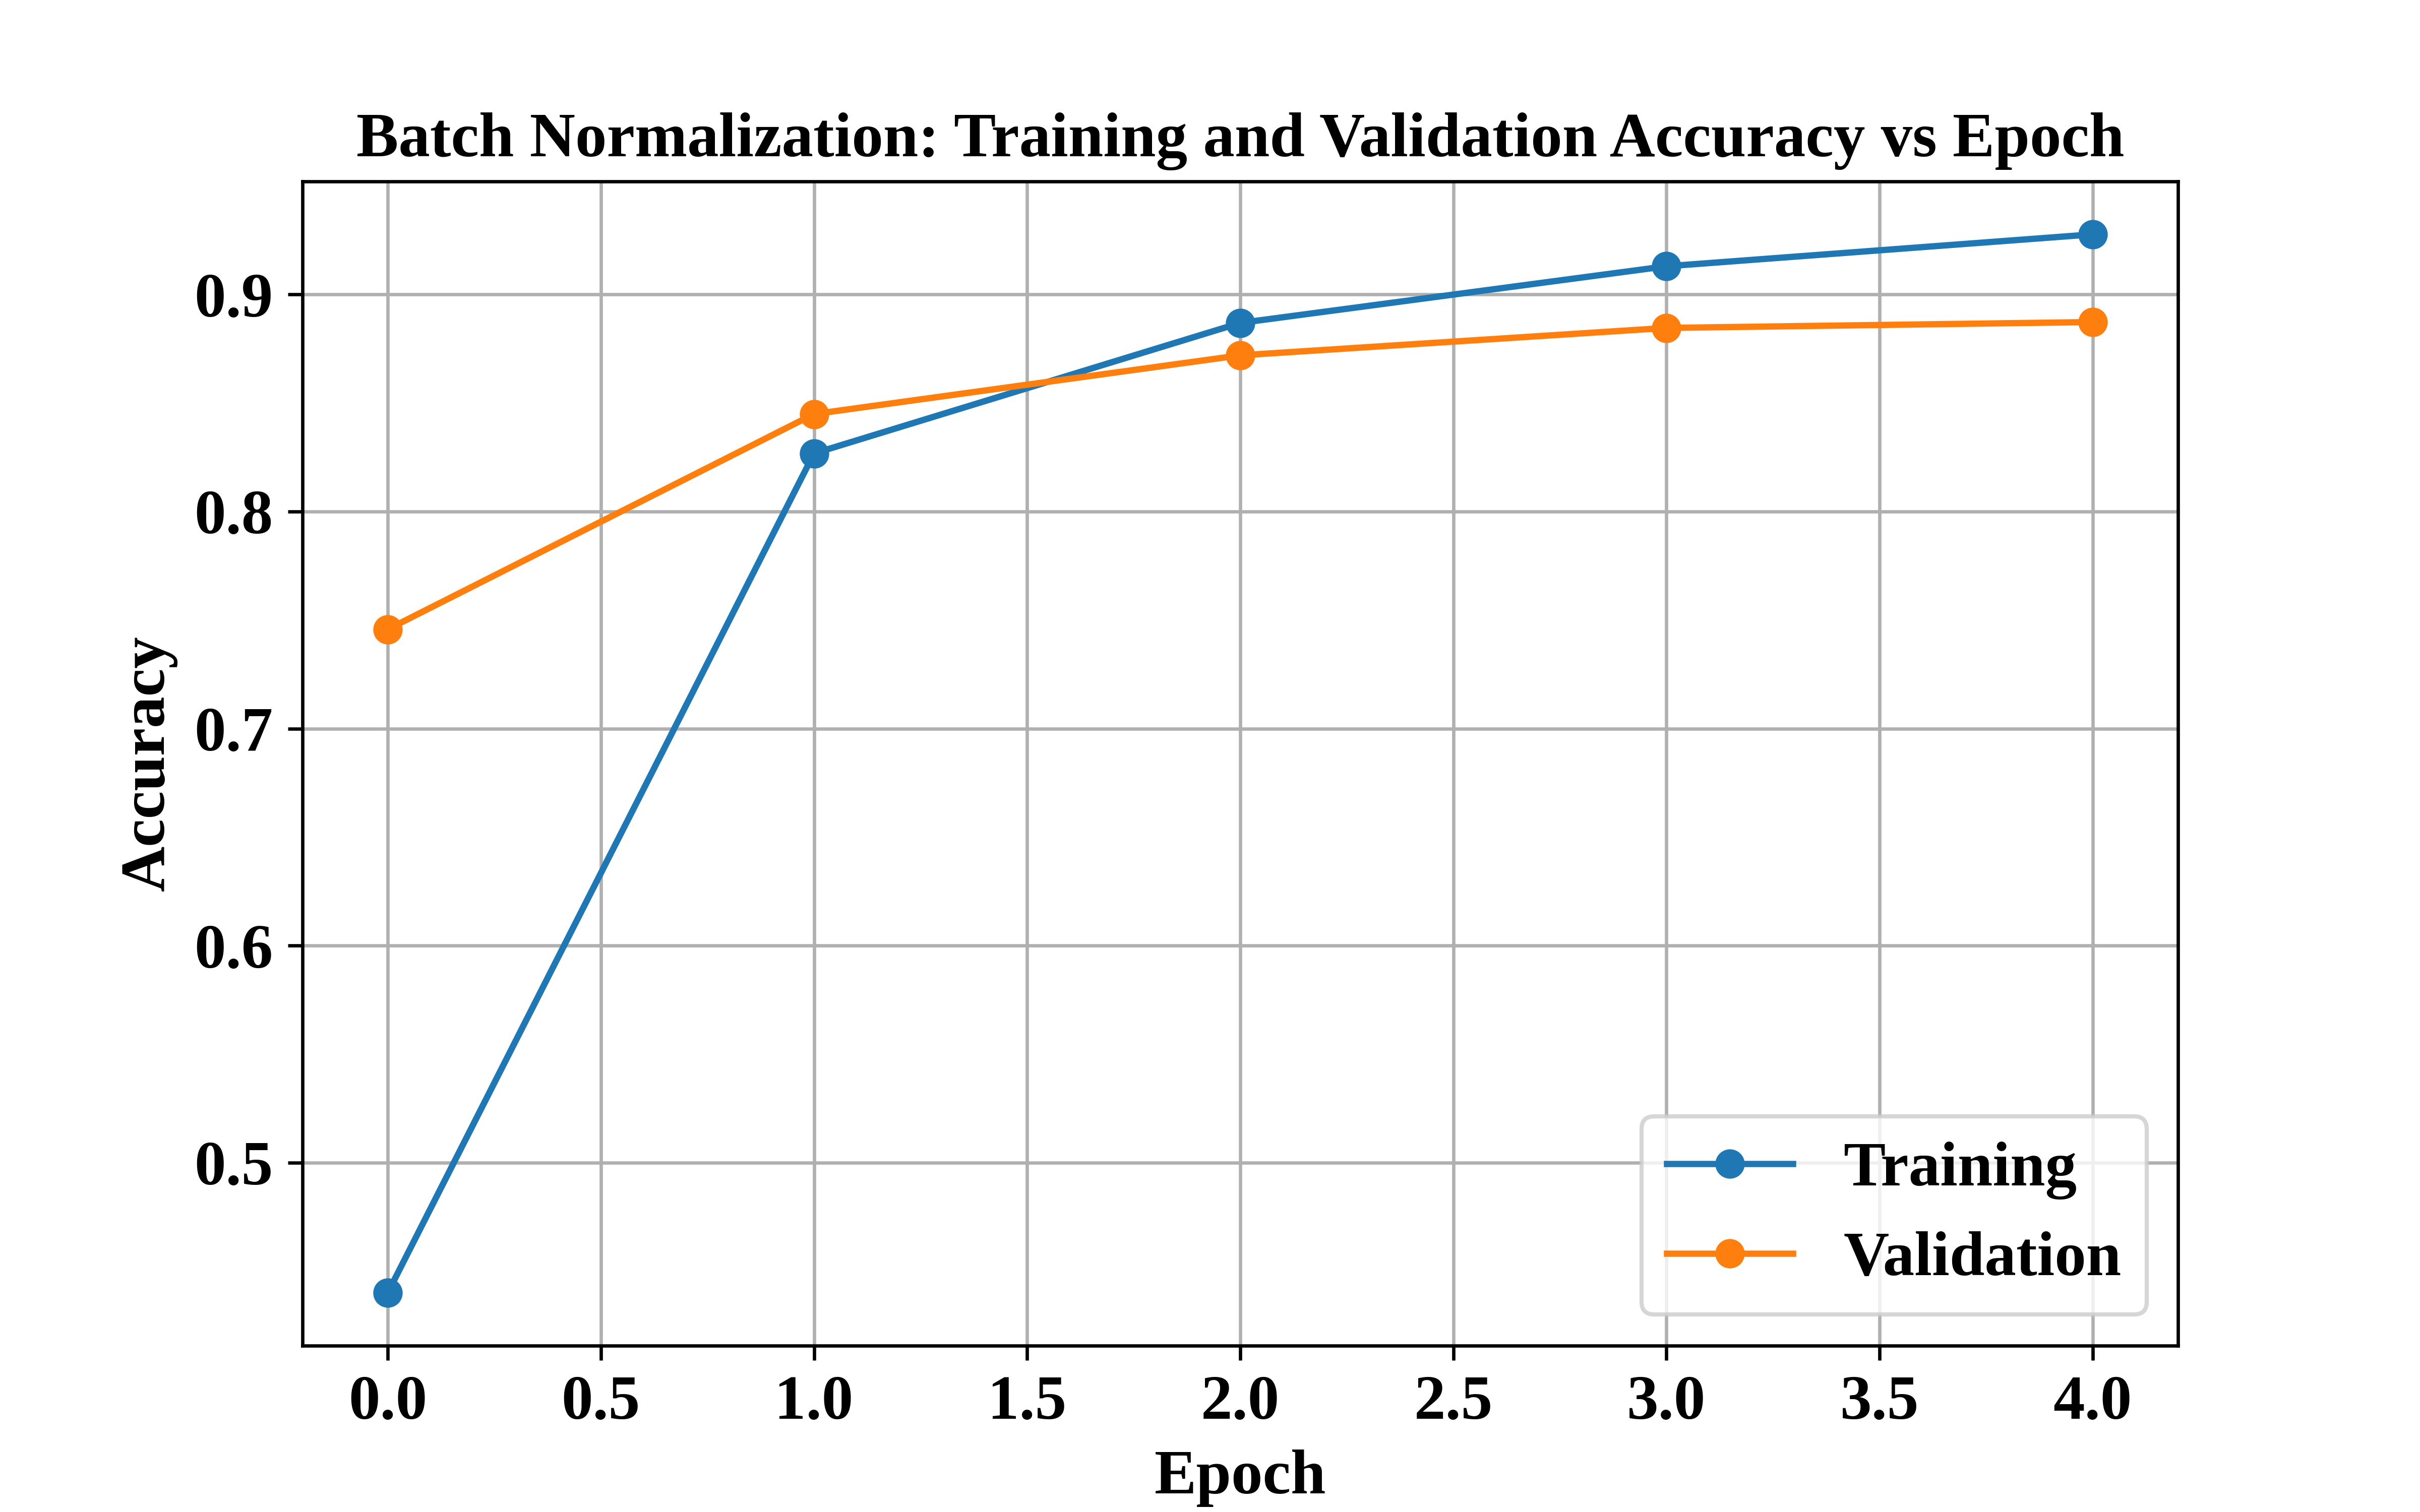
\includegraphics[width=1.0\textwidth]{Images/BatchNormalization_TrainingandValidationAccuracyvsEpoch.png}
            \caption{Training and Validation Accuracy vs Epoch}
            \label{fig:AccuracyBN}
        \end{minipage}
        \hfill
        \begin{minipage}{0.48\textwidth}
            \centering
            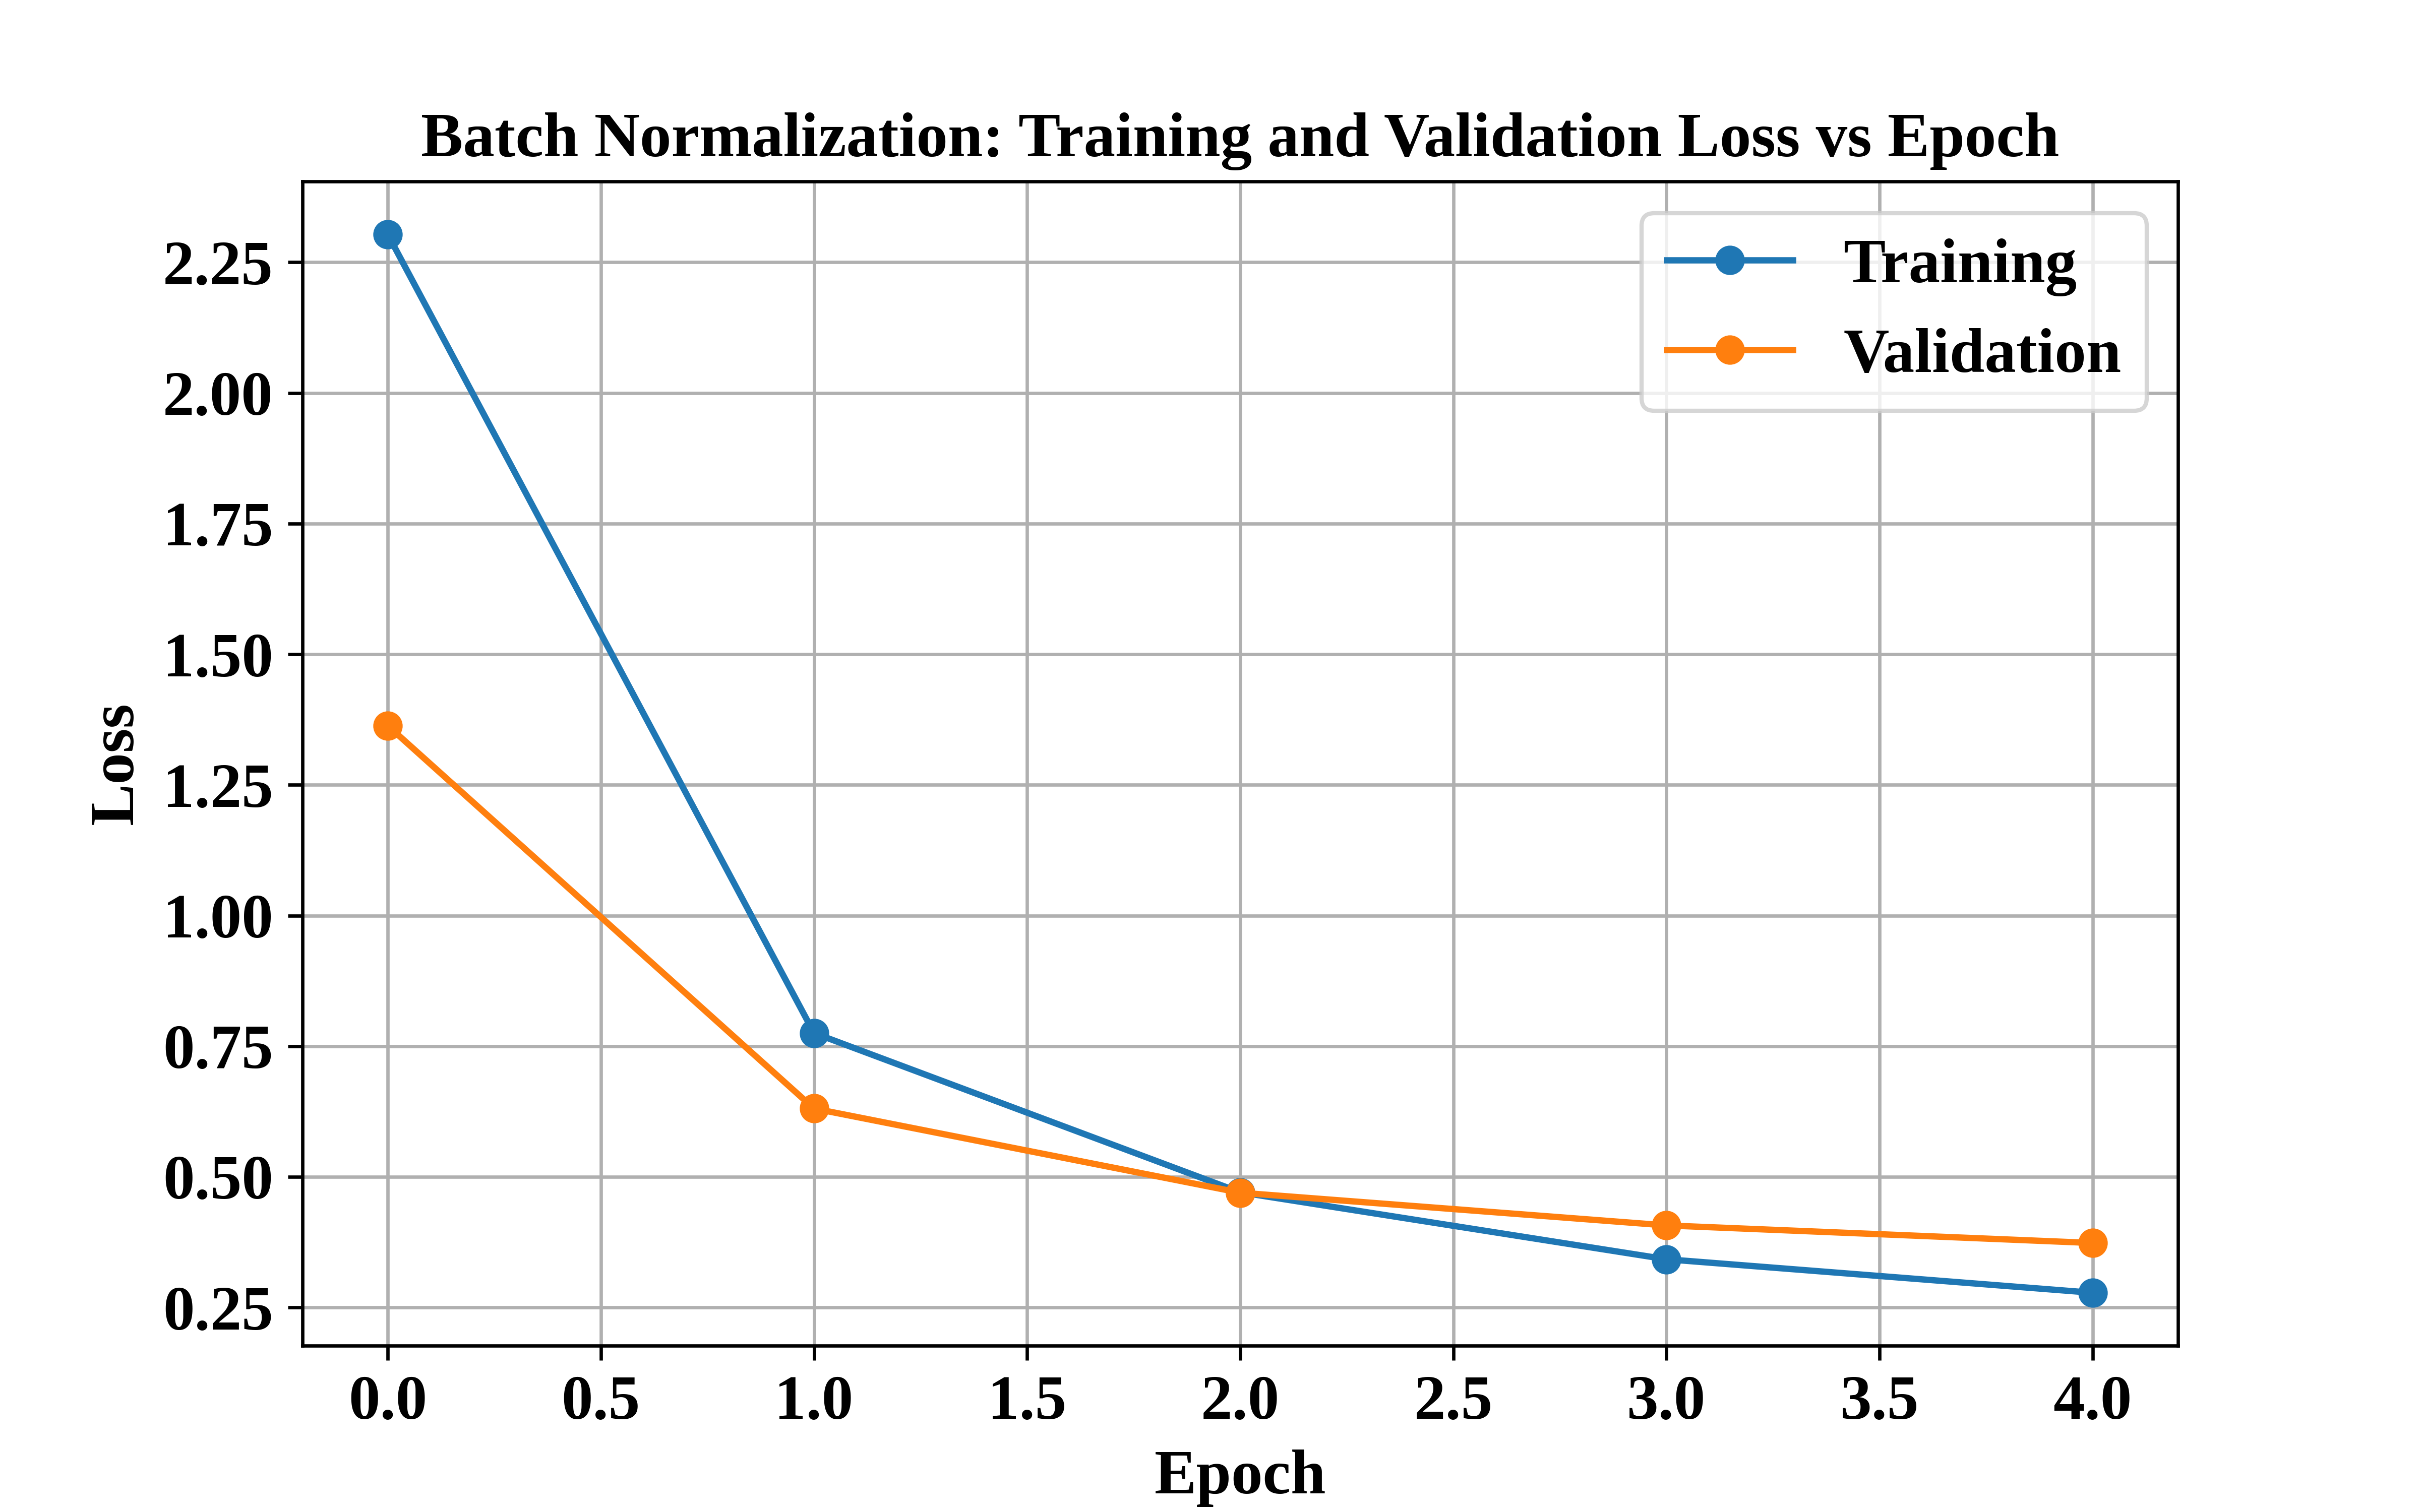
\includegraphics[width=1.0\textwidth]{Images/BatchNormalization_TrainingandValidationLossvsEpoch.png}
            \caption{Training and Validation Loss vs Epoch}
            \label{fig:LossBN}
        \end{minipage}

    \end{figure}
    \noindent\textbf{Training and Validation Accuracy vs Epoch Inference:}\\
    The plot compares training and validation accuracy across 5 epochs for models trained with batch normalization.
    Both the curves shows steady increase with validation curve having higher accuracy consistently.

    \vspace{5mm}
    \noindent\textbf{Training and Validation Loss vs Epoch Inference:}\\
    The plot compares training and validation loss across 5 epochs for models trained with batch normalization.
    Both the curves shows steady decrease with training curve having lower loss by the end of 5th epoch.

    \clearpage

    \item\textbf{With vs Without Batch Normalization}
        \begin{figure}[H]
        \centering
        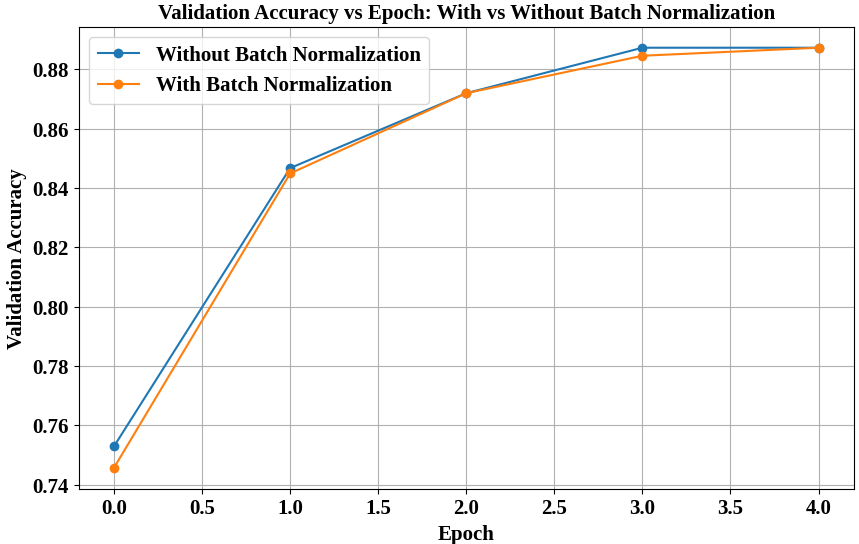
\includegraphics[width=0.8\textwidth]{Images/ValidationAccvsEpochWithWithoutBN.png}
        \caption{With vs Without Batch Normalization}
        \label{fig:ValidationAccvsEpochWithWithoutBN}
    \end{figure}
    \noindent\textbf{Inference:}\\
    The plot shows the validation accuracy of a model with batch normalization and without batch normalization across 5 epochs.
    Both configurations follows almost identical trajectories reaching approx. 89 percent validation accuracy by the end of 5 epochs.
    Batch Normalization primarily stabilizes deeper networks or higher learning rates. For simpler architectures with smaller learning rates standard optimization already stabilizes quickly without extra normalization layers.

    \clearpage

    \item\textbf{Training Loss vs. Epoch for Different Optimizers}
        \begin{figure}[H]
        \centering
        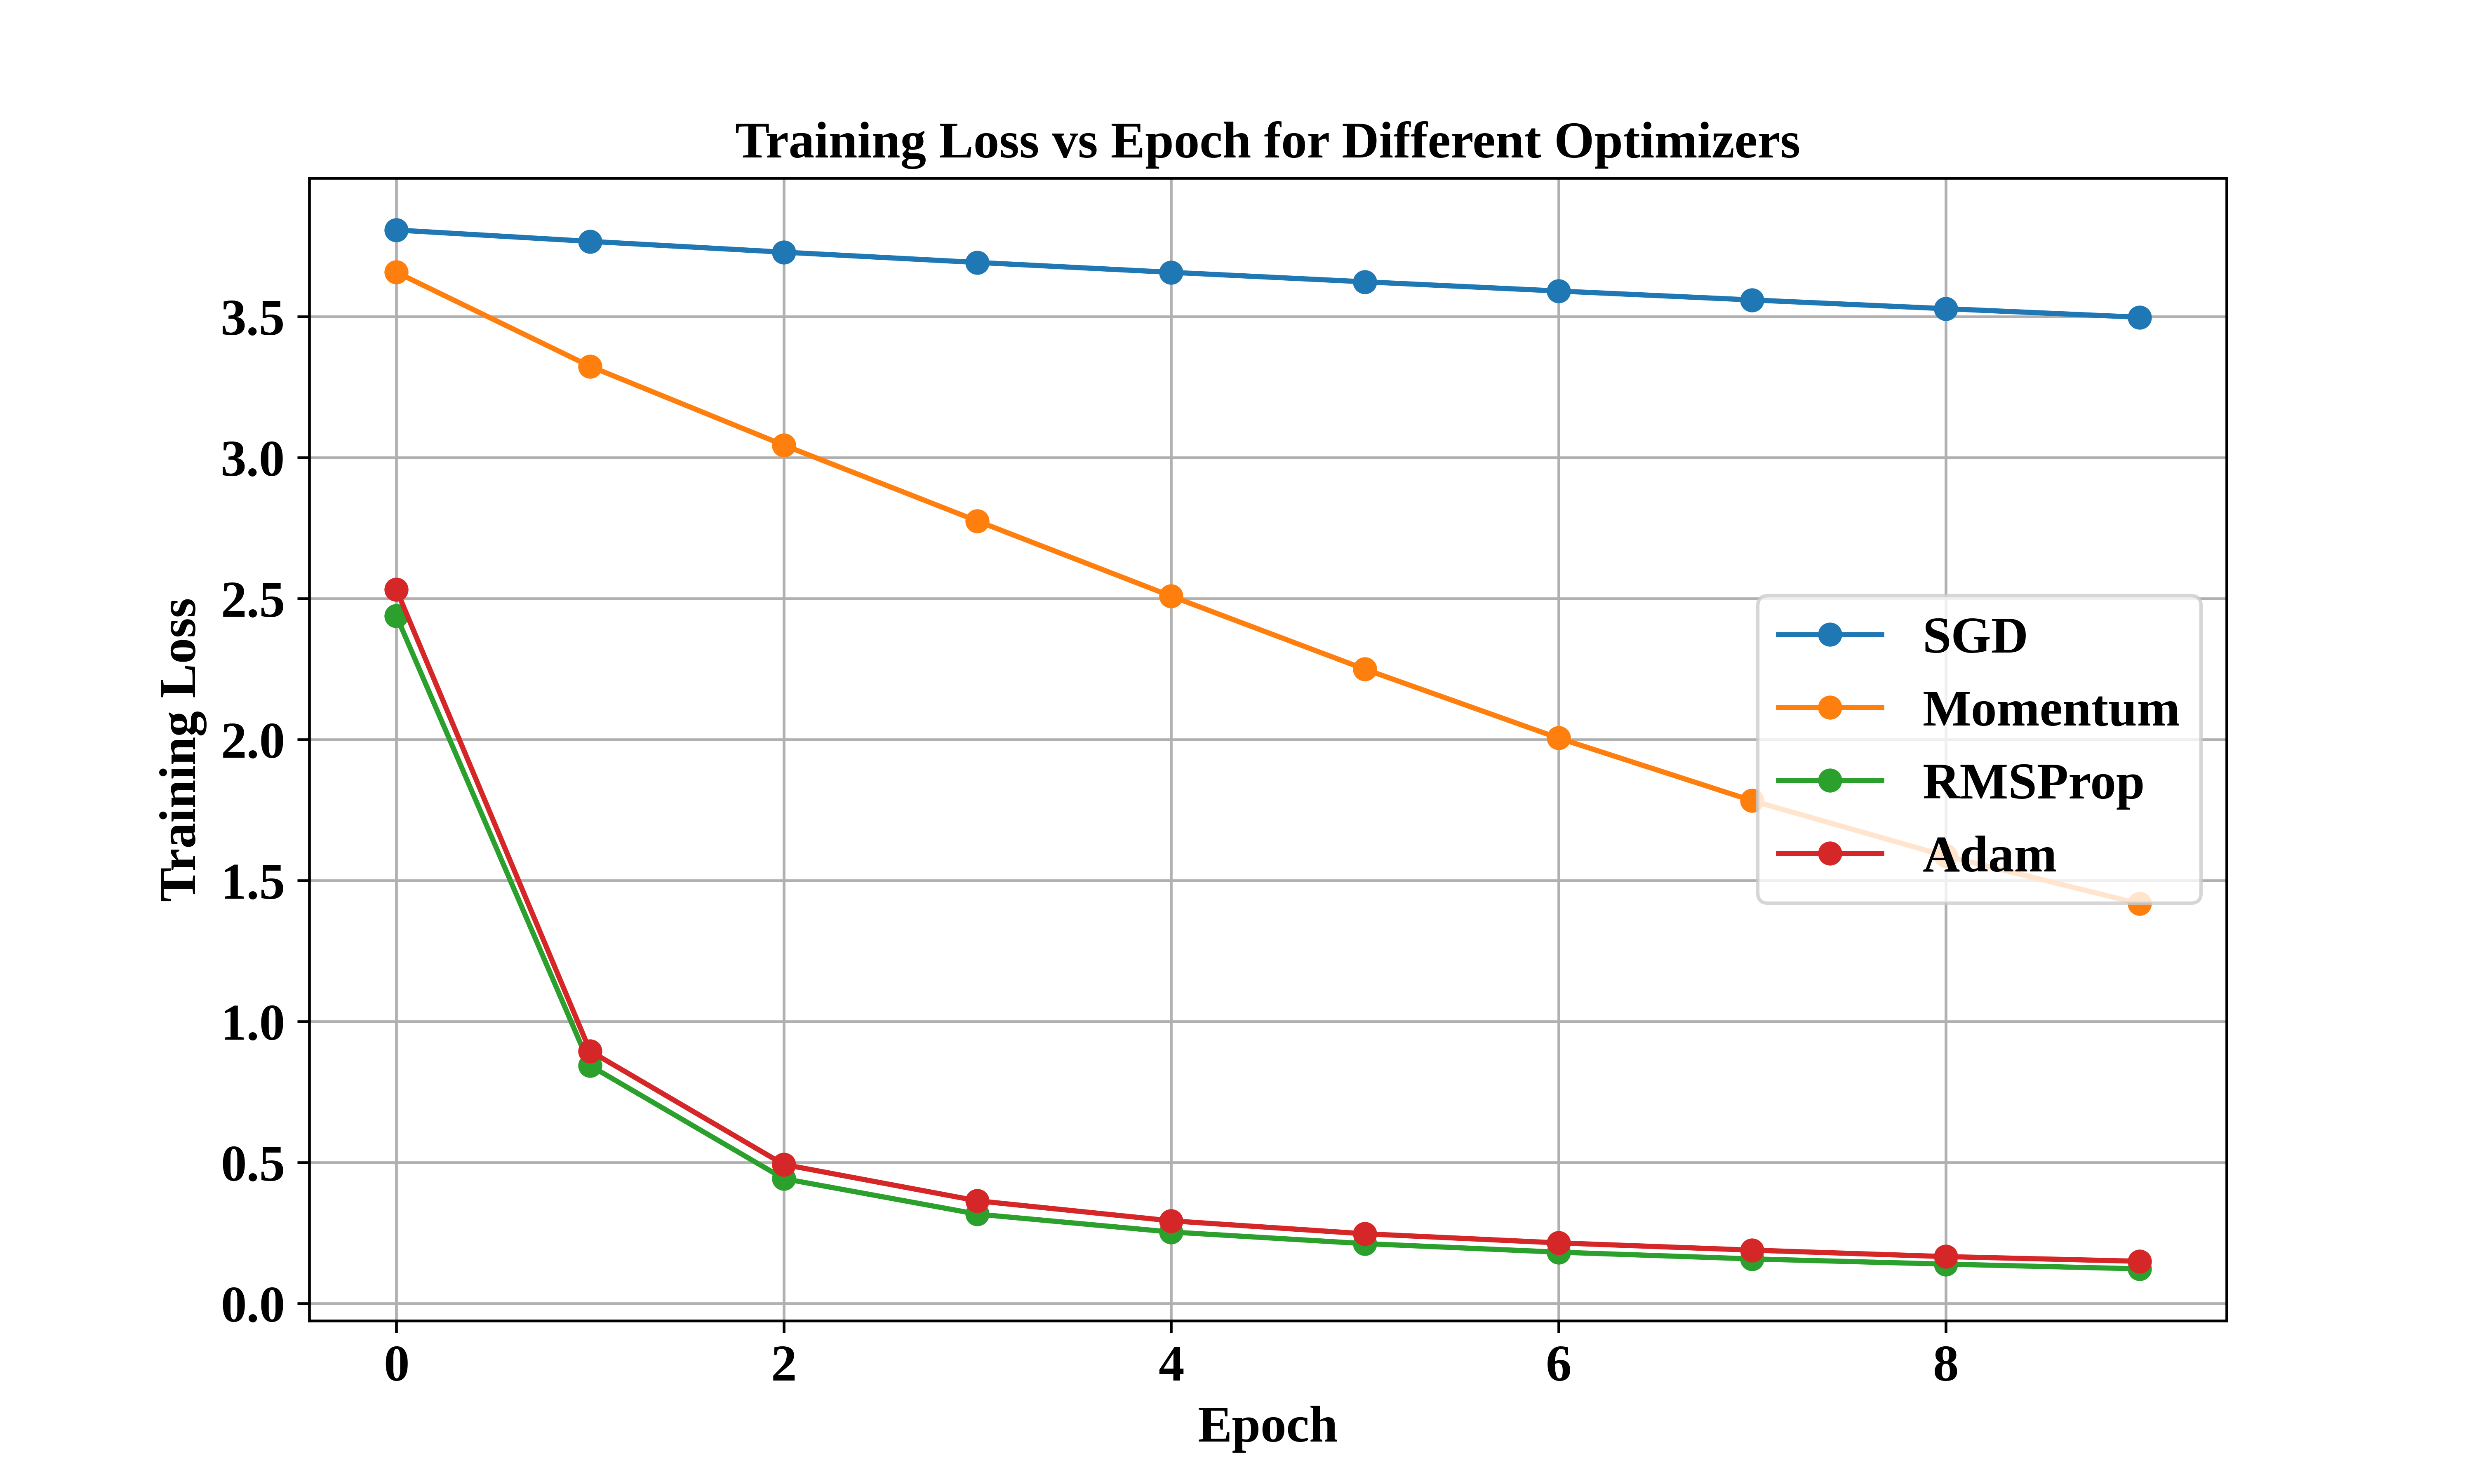
\includegraphics[width=0.8\textwidth]{Images/TrainingLossvsEpochforDifferentOptimizers.png}
        \caption{Training Loss vs. Epoch for Different Optimizers}
        \label{fig:TrainingLossvsEpochforDifferentOptimizers}
    \end{figure}
    \noindent\textbf{Inference:}\\
    The plot compares the training loss of four optimization algorithms such as SGD, Momentum, RMSProp, Adam across 10 epochs.
    RMSProp and Adam experience a sharp drop in training loss within the first two epochs and reach a steady training loss.
    Momentum displays a steady linear decrease in training loss reaching a minimum of 1.5. SGD shows highest training loss of 3.5 byt the end of 10 epochs.
    Adaptive optimizers such as Adam and RMSProp dynamically update learning rates for each parameter. Hence they show rapid decrease in training loss. 
    Momentum uses accumulated velocity to maintain steady updates, whereas SGD is shows poor performance due to inefficient step sizes. 
    
    \clearpage

    \item\textbf{Validation Accuracy vs. Epoch for Different Optimizers}
        \begin{figure}[H]
        \centering
        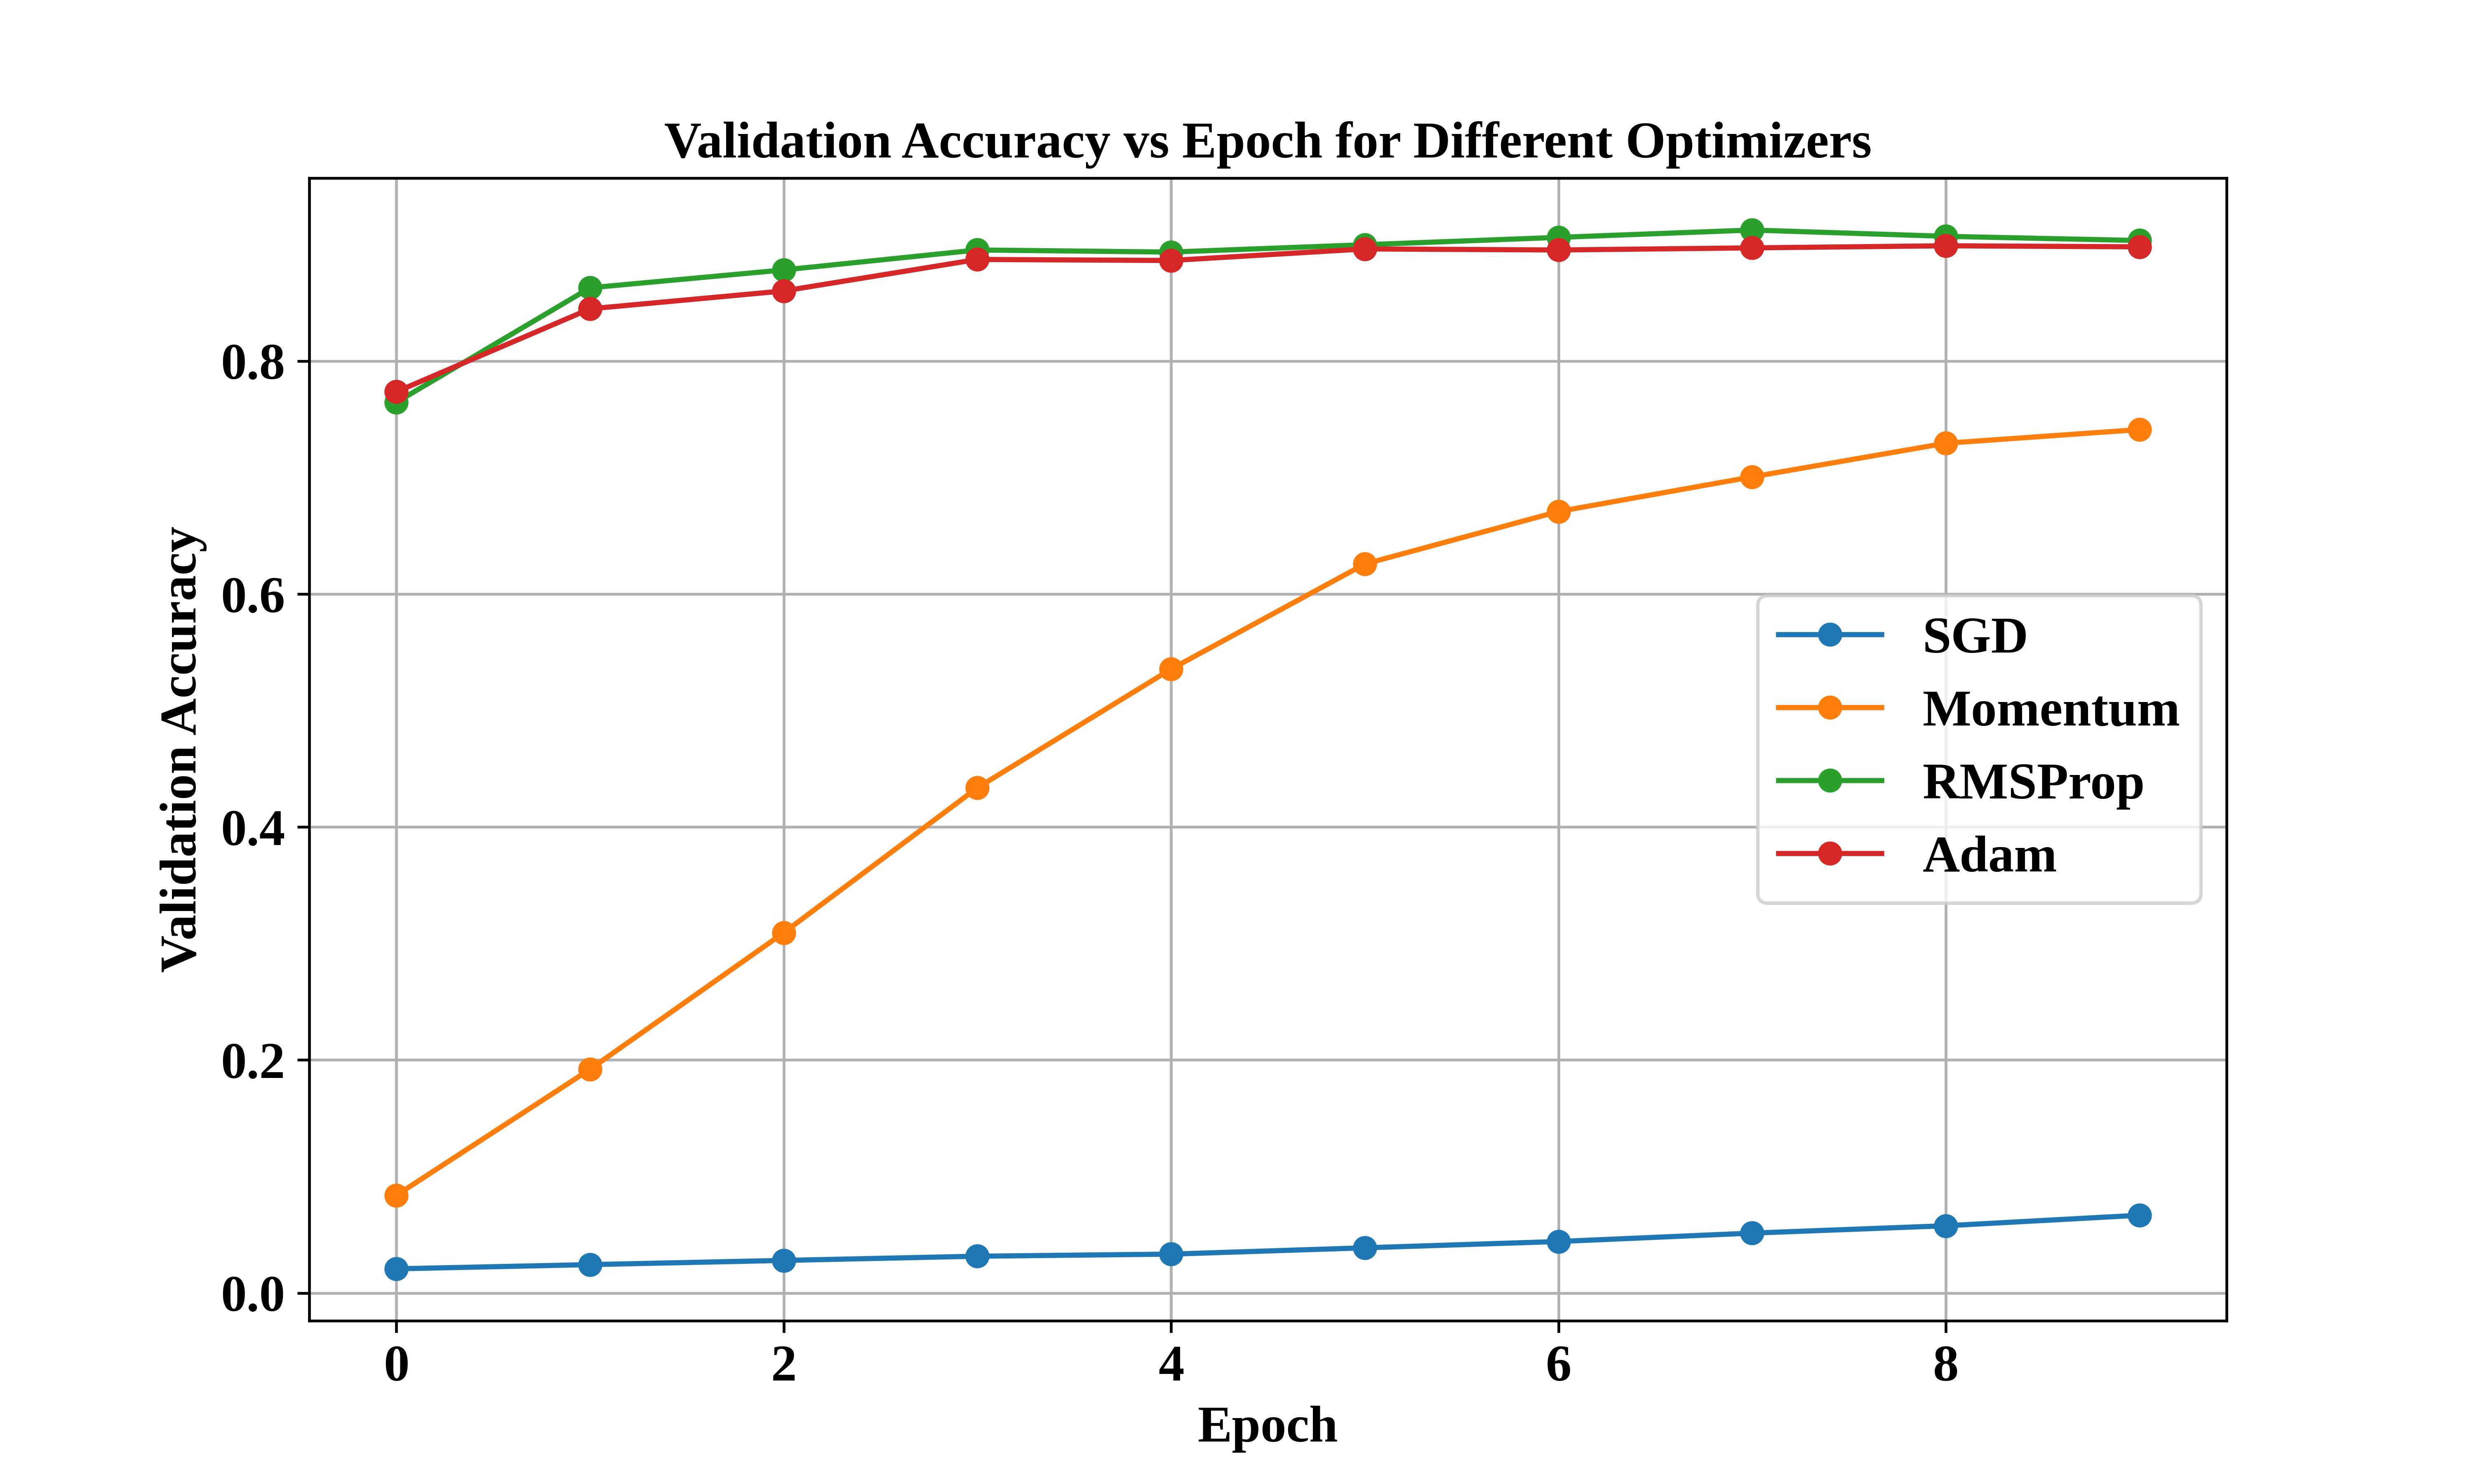
\includegraphics[width=0.8\textwidth]{Images/ValidationAccuracyvsEpochforDifferentOptimizers.png}
        \caption{Validation Accuracy vs. Epoch for Different Optimizers}
        \label{fig:ValidationAccuracyvsEpochforDifferentOptimizers}
    \end{figure}
    \noindent\textbf{Inference:}\\
    The plot compares the validation accuracy of four optimization algorithms such as SGD, Momentum, RMSProp, Adam across 10 epochs.
    Adaptive optimizers such as Adam and RMSProp achieve rapid early convergence with high accuracy of approx. 85 percent. Momentum exhibits steady, moderate growth while SGD performs poorly with under 10 percent accuracy.
    This trend is observed because Adam and RMSProp dynamically adapt learning rates for individual parameters to quickly navigate steep gradients. Momentum uses velocity to accelerate past gradients, whereas SGD uses a fixed learning rate that struggles to make progress.
    
    \clearpage

    \item\textbf{Dropout Rate vs Validation Accuracy}
        \begin{figure}[H]
        \centering
        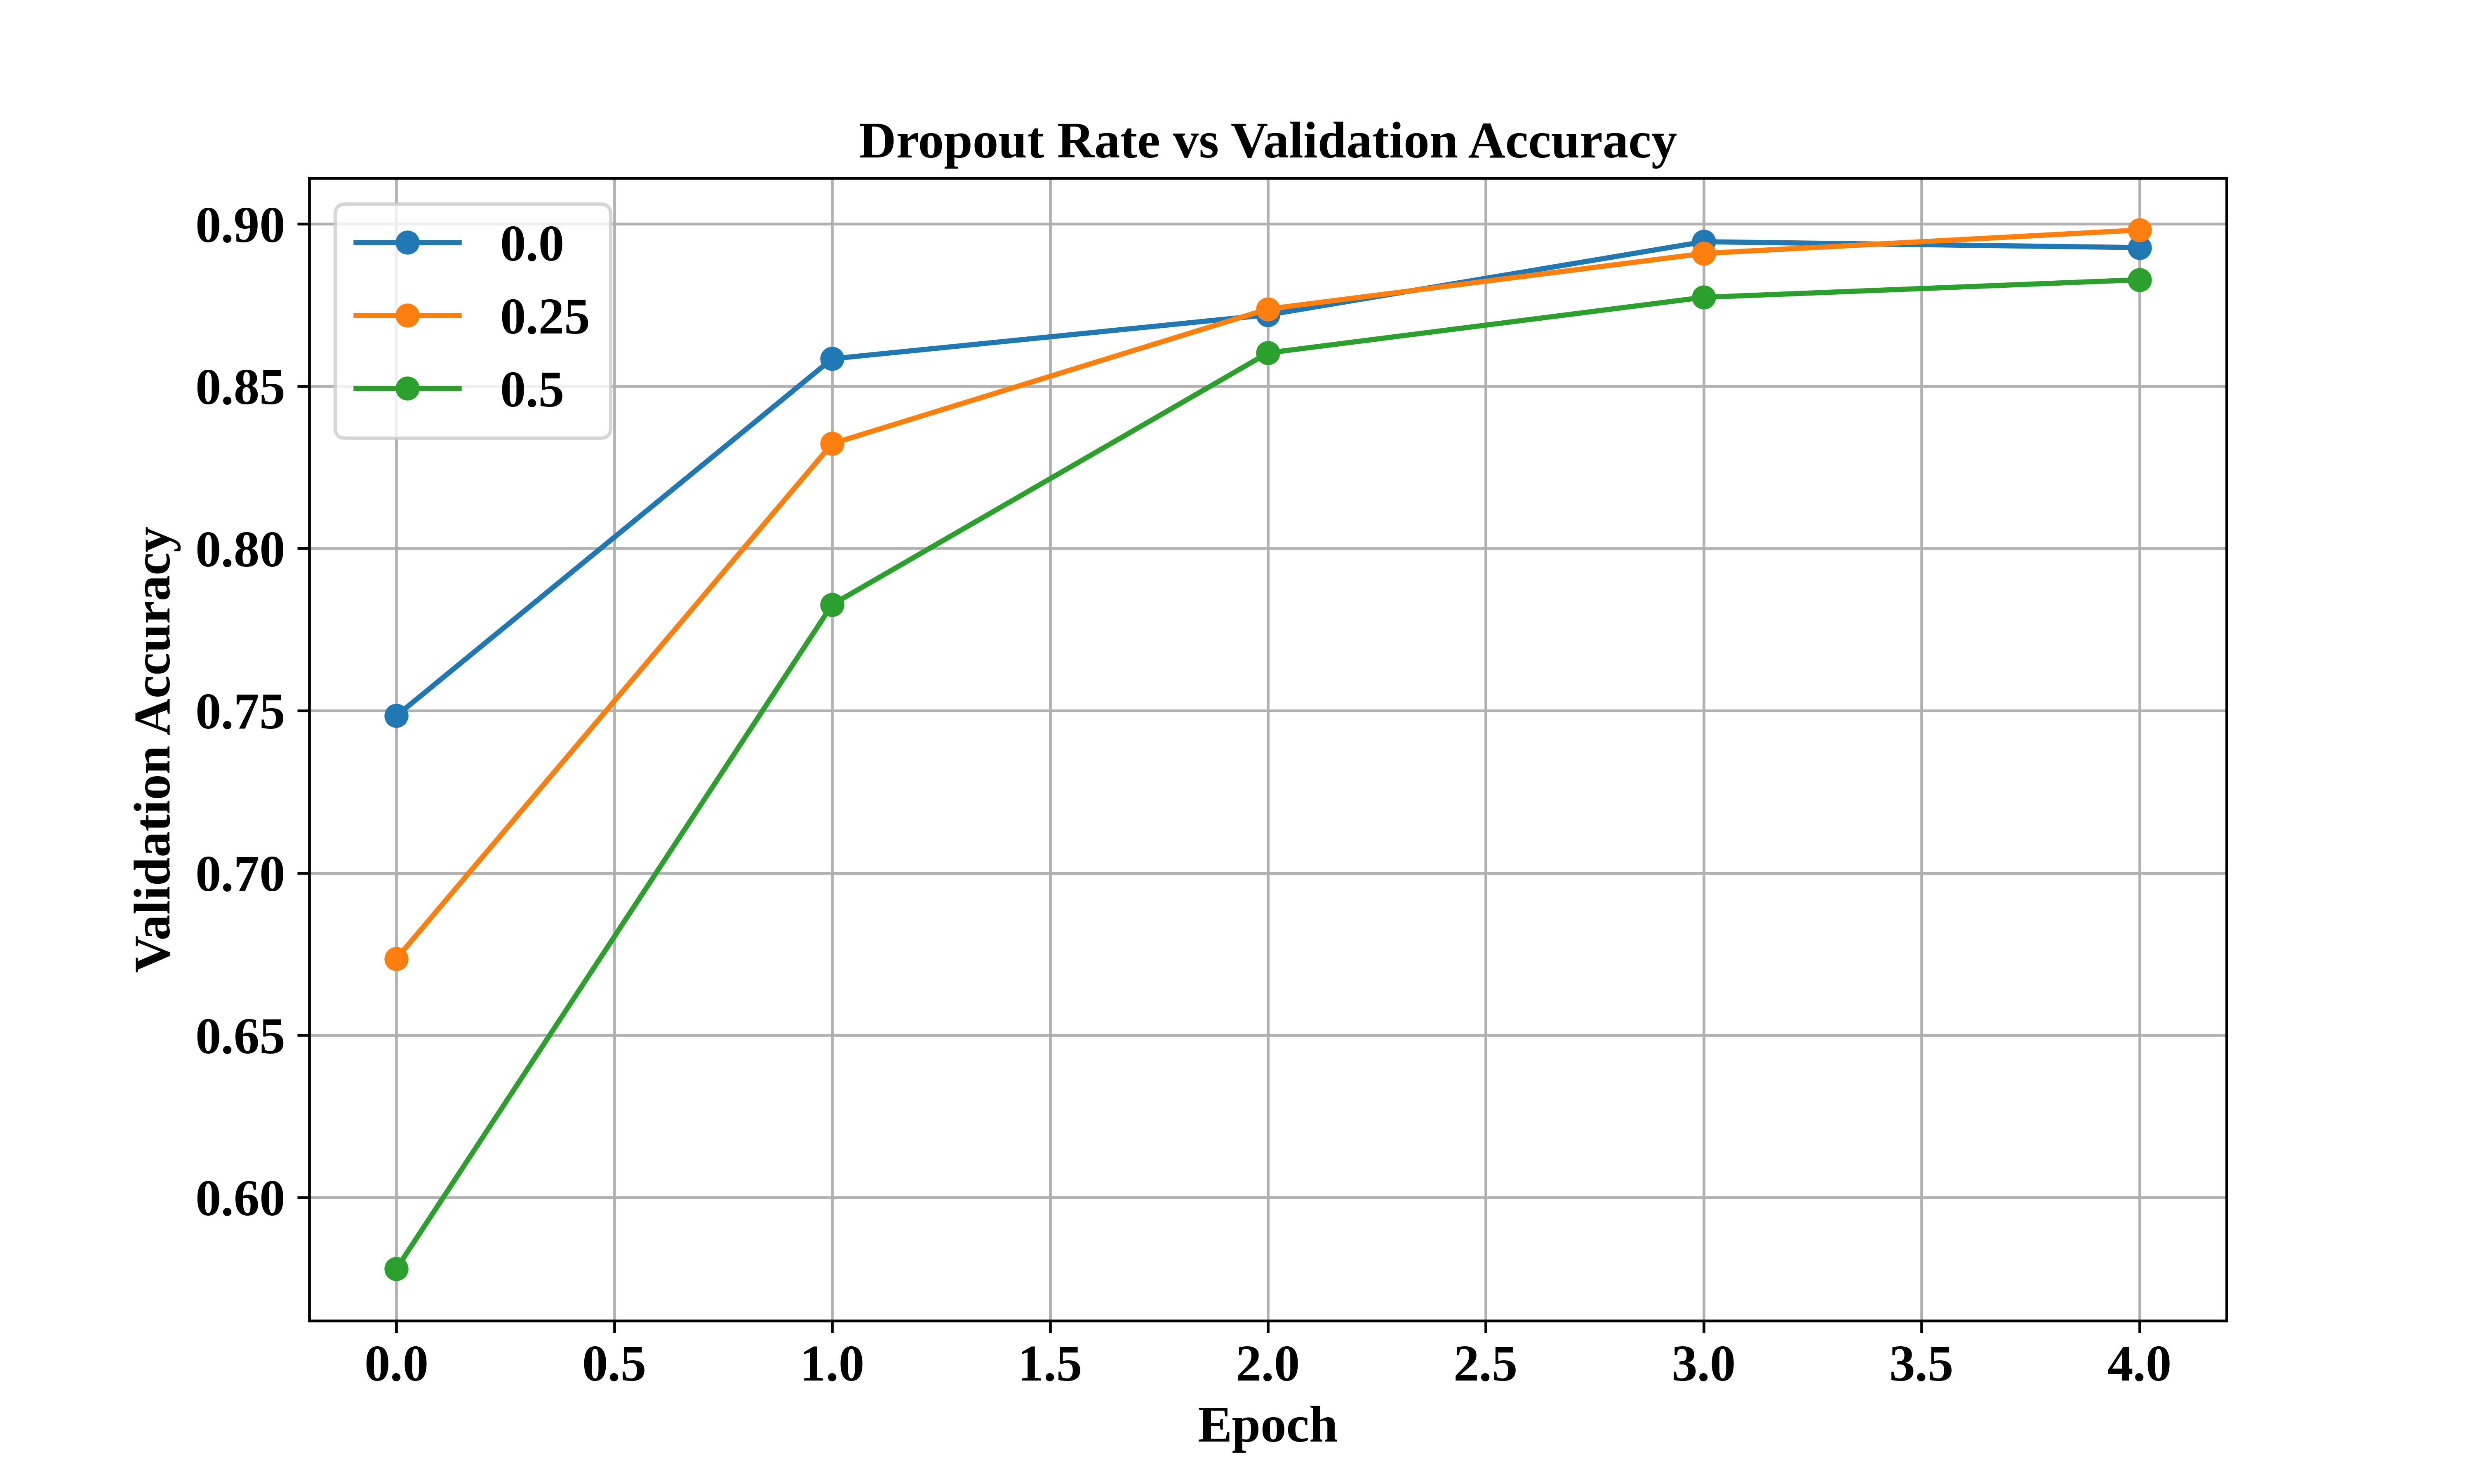
\includegraphics[width=0.8\textwidth]{Images/DropoutRatevsValidationAccuracy.png}
        \caption{Dropout Rate vs Validation Accuracy}
        \label{fig:DropoutRatevsValidationAccuracy}
    \end{figure}
    \noindent\textbf{Inference:}\\
    The plot shows the comparison of validation accuray for different dropout rates (dropout rate = 0.0, 0.25, 0.5) over 5 epochs.
    Initially, no dropout shows highest validation accuracy. By the end of 5th epoch, model with dropout rate = 0.25 reaches the highest validation accuracy. 
    The model with dropout rate = 0.5 has the lowest validation accuracy. 
    By preventing neurons from co-adapting and relying on specific features, dropout rate = 0.25 reduces overfitting and allows the network to generalize better.

    \clearpage

    \item\textbf{Feature Extraction vs. Fine-Tuning}
        \begin{figure}[H]
        \centering
        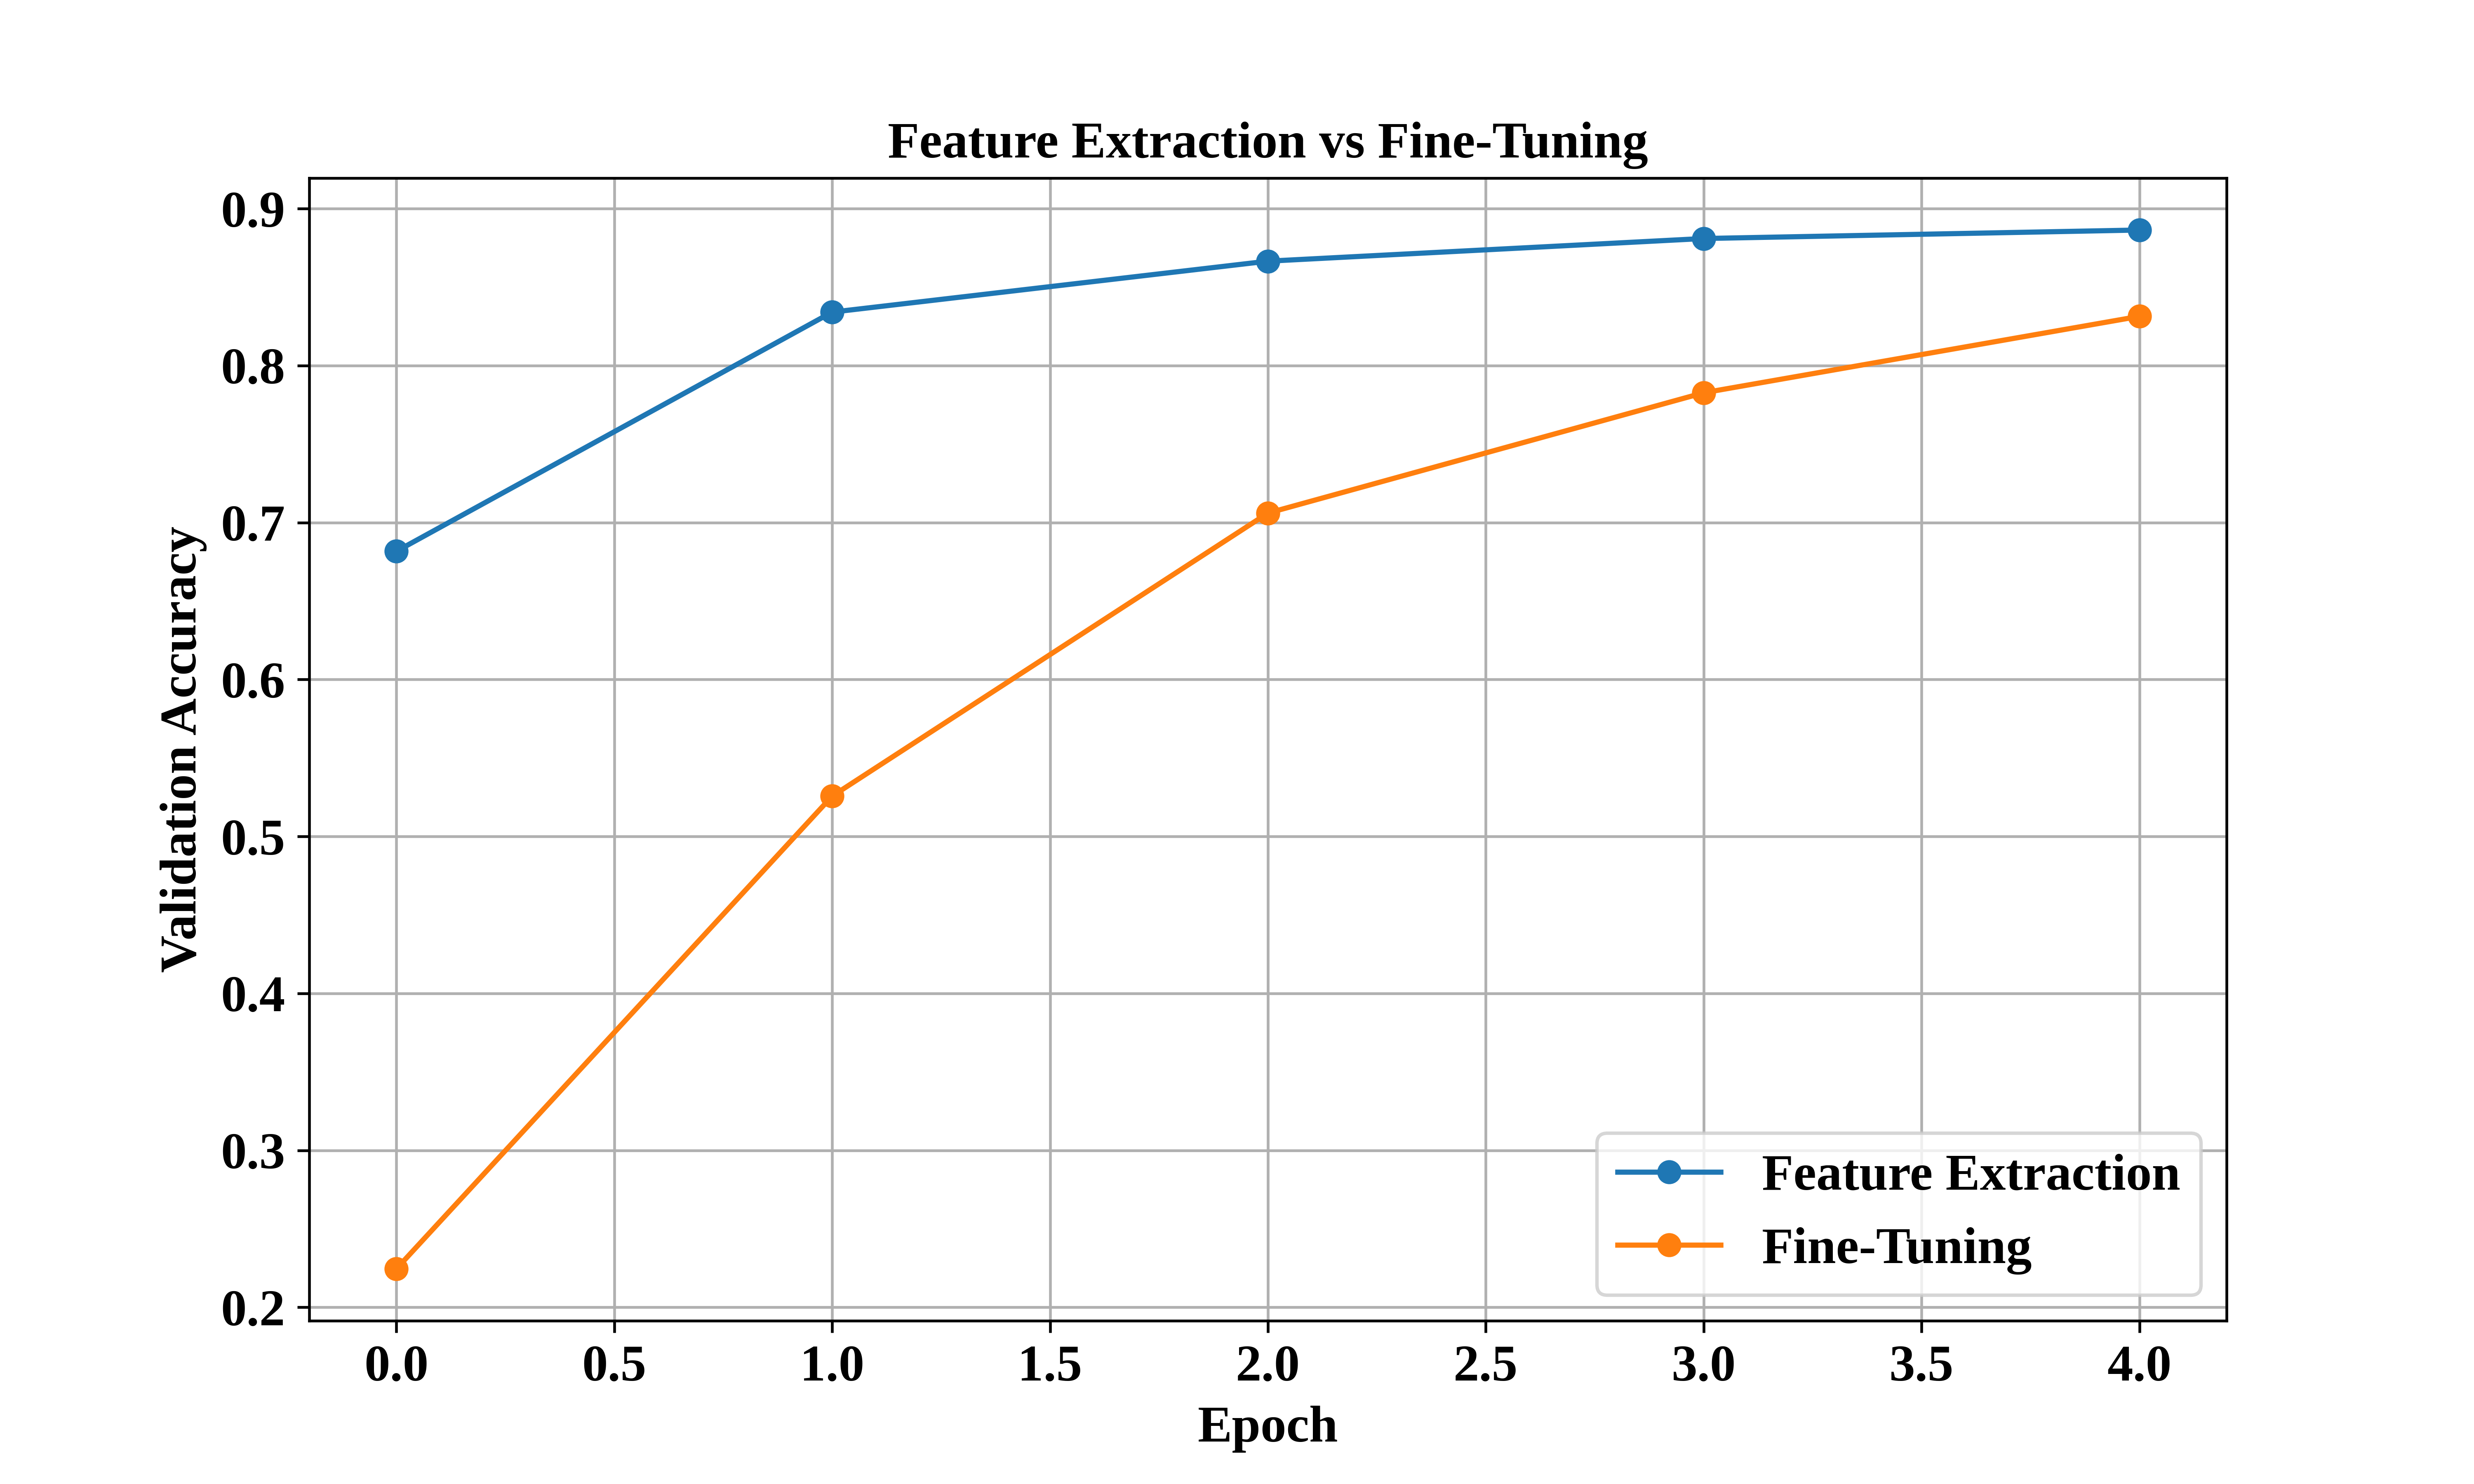
\includegraphics[width=0.8\textwidth]{Images/FeatureExtractionvsFine-Tuning.png}
        \caption{Feature Extraction vs. Fine-Tuning}
        \label{fig:FeatureExtractionvsFine}
    \end{figure}
    \noindent\textbf{Inference:}\\
    The plot shows the comparison of feature extraction and fine tuning.
    Feature Extraction starts at a much higher initial validation accuracy and maintains a clear accuracy advantage across all 5 epochs, reaching approx. 89 percent compared to Fine-Tuning's 80 percent.
    Feature Extraction freezes the feature extractor layers, preserving the strong general visual representations while only updating the final classification head. This prevents early instability.
    Unfreezing base layers during fine tuning can cause catastrophic forgetting of pre-trained features. Hence it requires larger initial weight updates or smaller learning rate and more epochs to converge.

    \clearpage

    \item \textbf{Training and Validation Loss for Feature Extraction and Fine Tuning}

    \begin{figure}[H]
        \centering

        \begin{minipage}{0.48\textwidth}
            \centering
            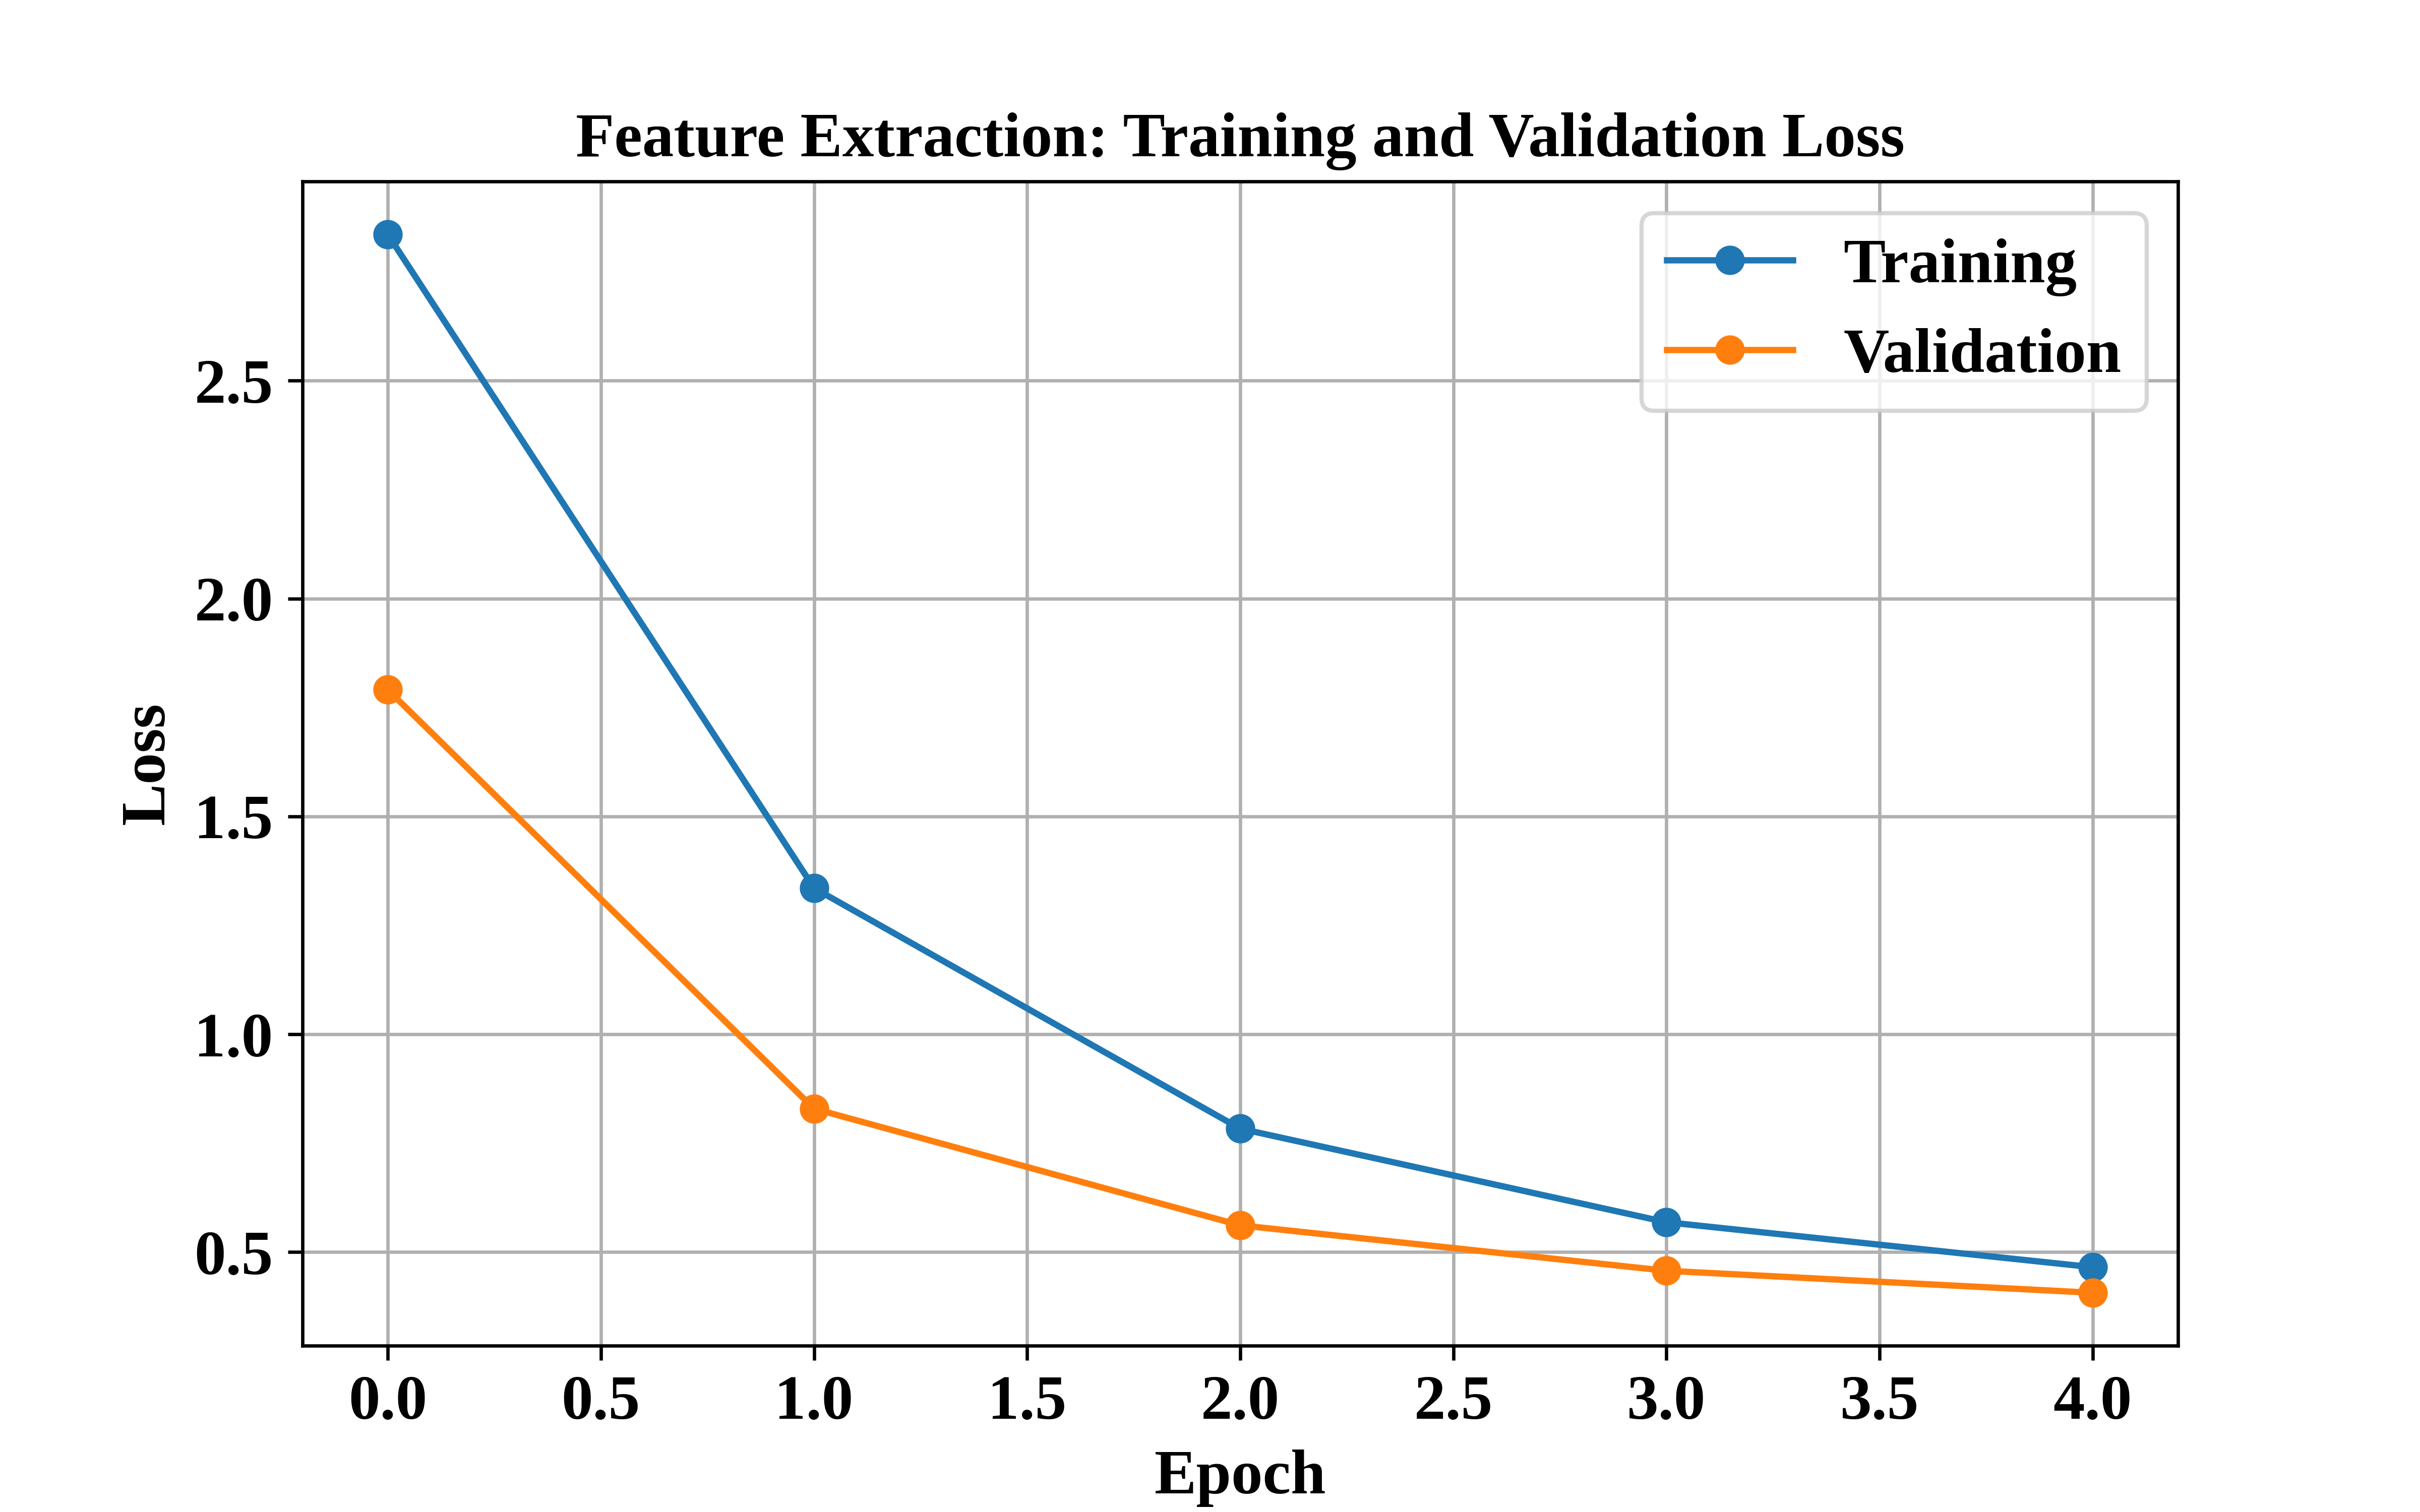
\includegraphics[width=1.0\textwidth]{Images/FeatureExtraction_TrainingandValidationLoss.png}
            \caption{Feature Extraction}
            \label{fig:AccuracyBN}
        \end{minipage}
        \hfill
        \begin{minipage}{0.48\textwidth}
            \centering
            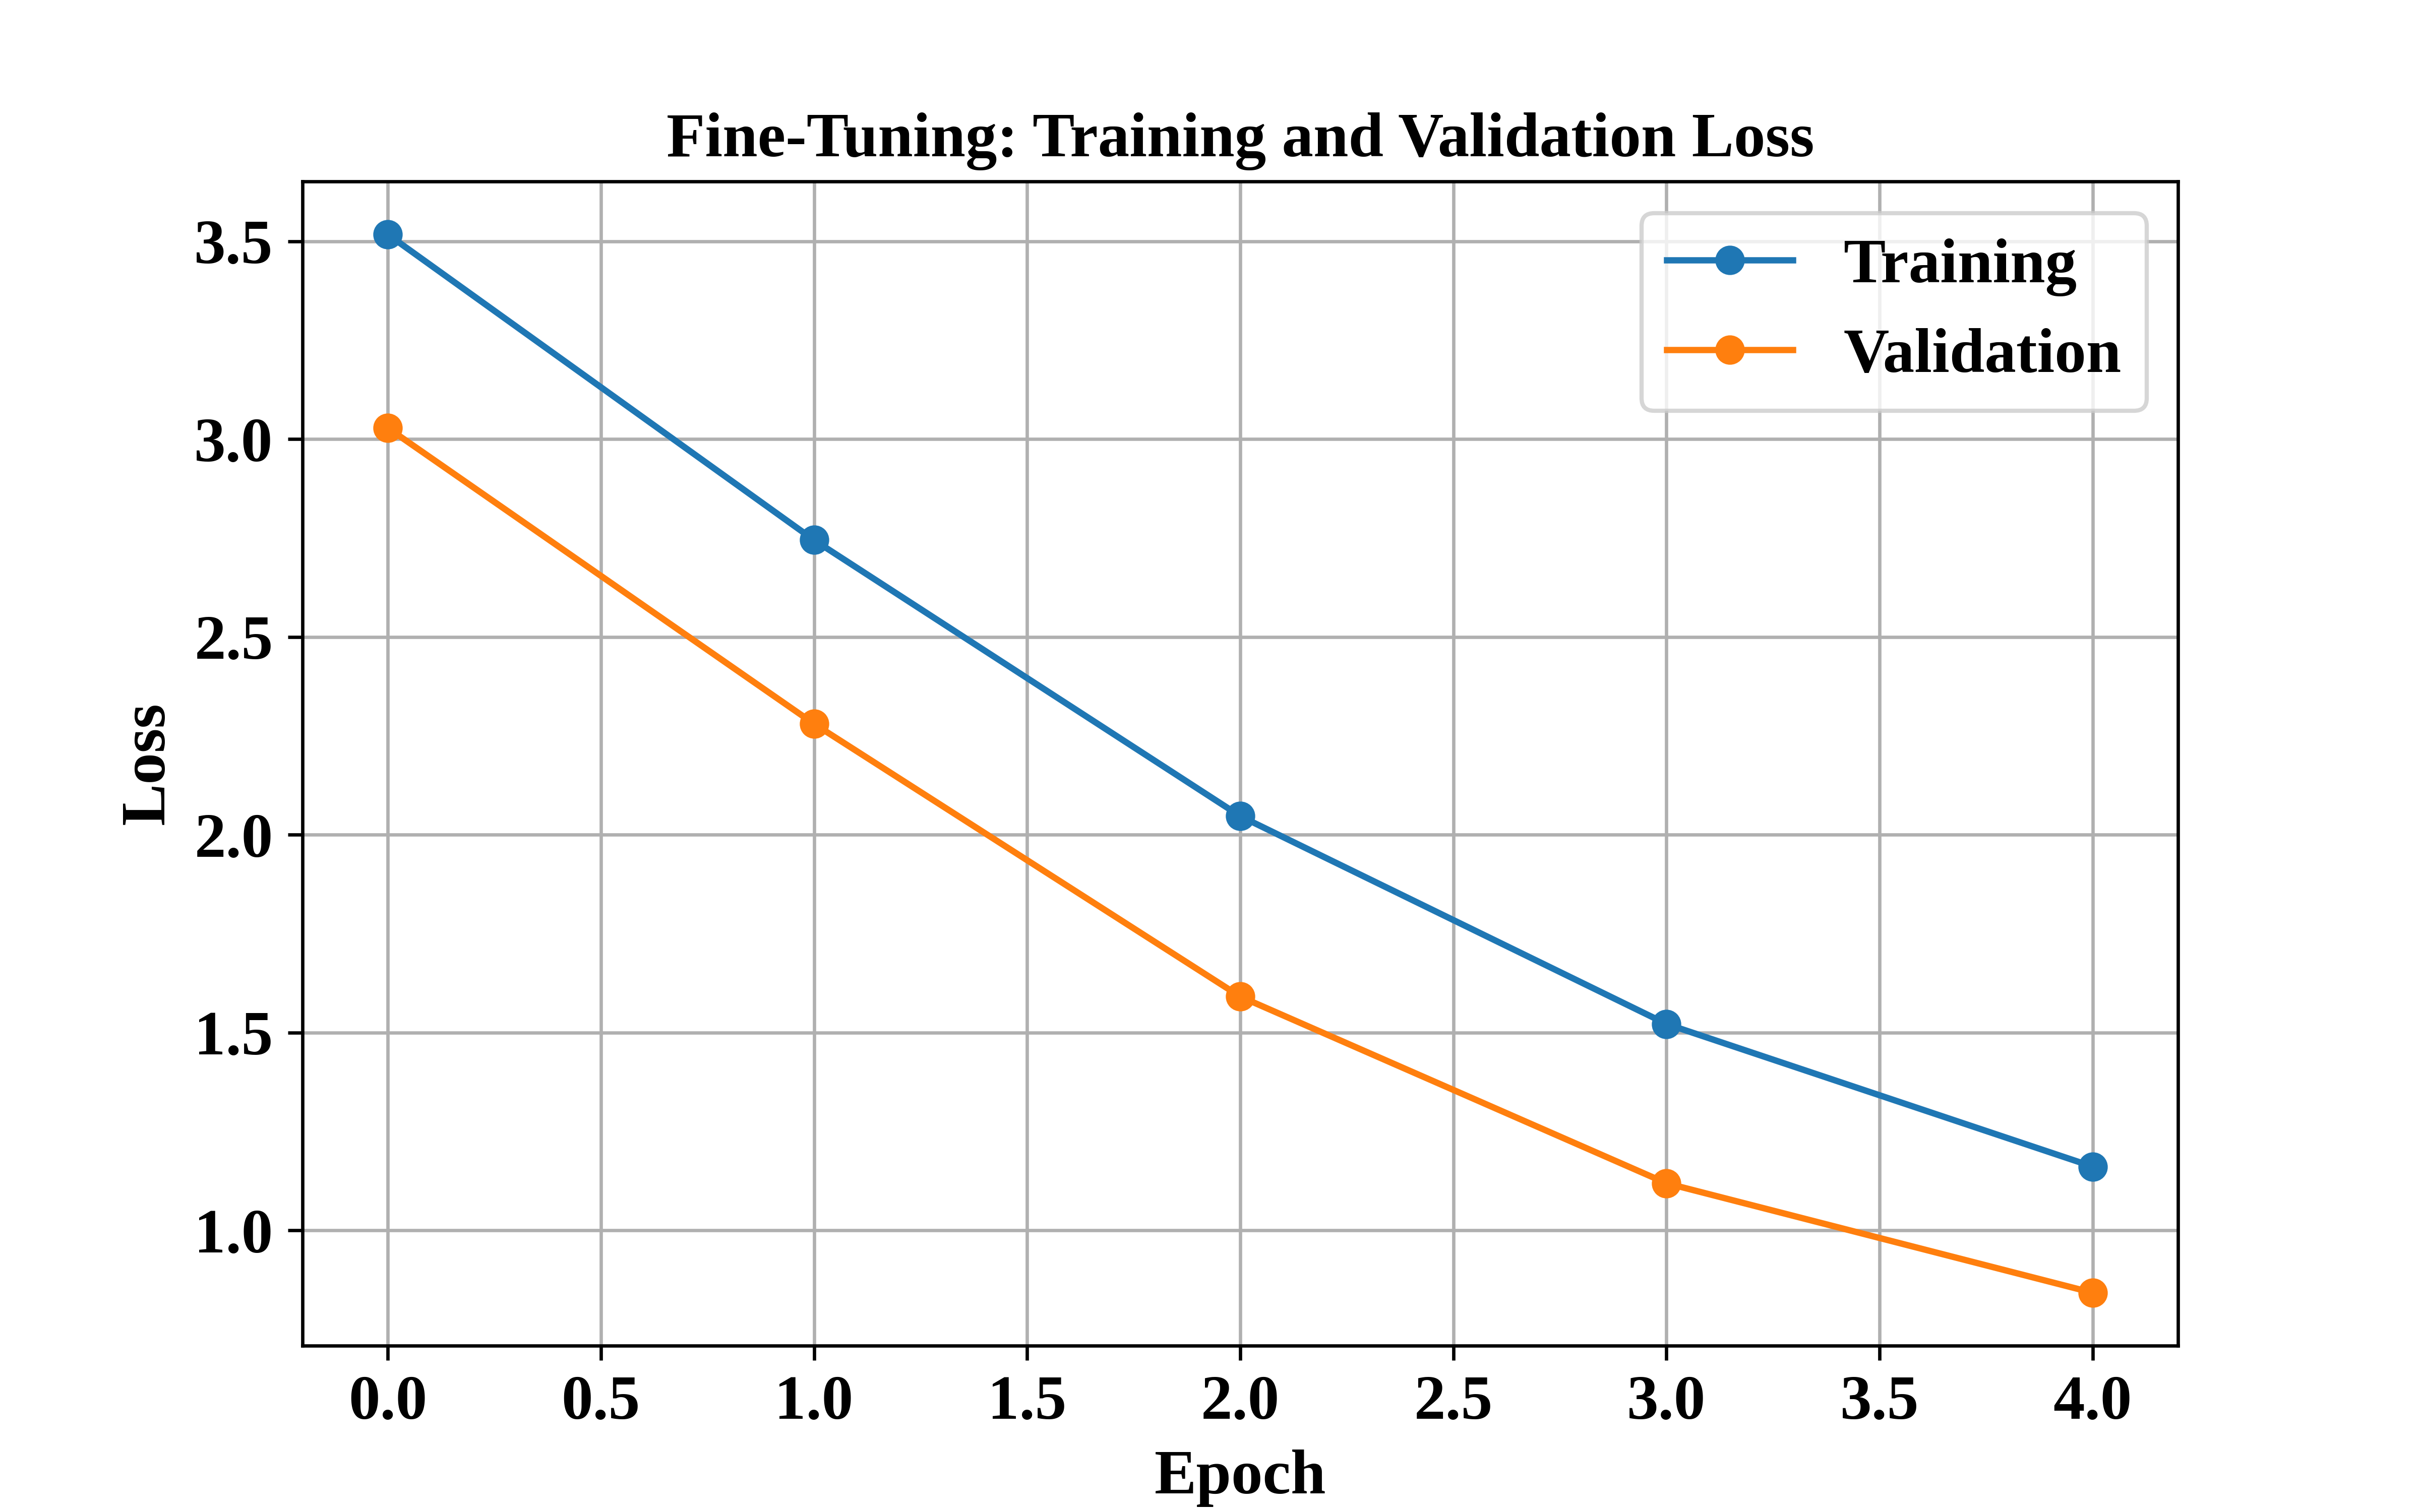
\includegraphics[width=1.0\textwidth]{Images/Fine-Tuning_TrainingandValidationLoss.png}
            \caption{Fine Tuning}
            \label{fig:LossBN}
        \end{minipage}

    \end{figure}
    \noindent\textbf{Feature Extraction: Training and Validation Loss vs Epoch Inference:}\\
    The plot shows the steady decrease in Training and Validaiton loss curves for feature extraction.
    The training loss is higher than validation loss in the earlier epochs. By the end of 4th epoch, both the loss values converge at 0.5.
    The steady decline indicates that the model is actively learning target features without overfitting.
    Validation loss is often lower than training loss because training loss is averaged during an epoch while the model is still updating, whereas validation loss is measured after the epoch's weight updates.
    
    \vspace{5mm}

    \noindent\textbf{Fine Tuning: Training and Validation Loss vs Epoch Inference:}\\
    The plot shows the Training and Validaiton loss curves for fine tuning.
    Both training and validation loss decrease smoothly and consistently over time.
    Validation loss remains consistently lower than training loss throughout all epochs.
    The steady decline indicates that the model is actively learning target features without overfitting.
    
    \clearpage
    \item\textbf{5-Fold Cross Validation Accuracy}
        \begin{figure}[H]
        \centering
        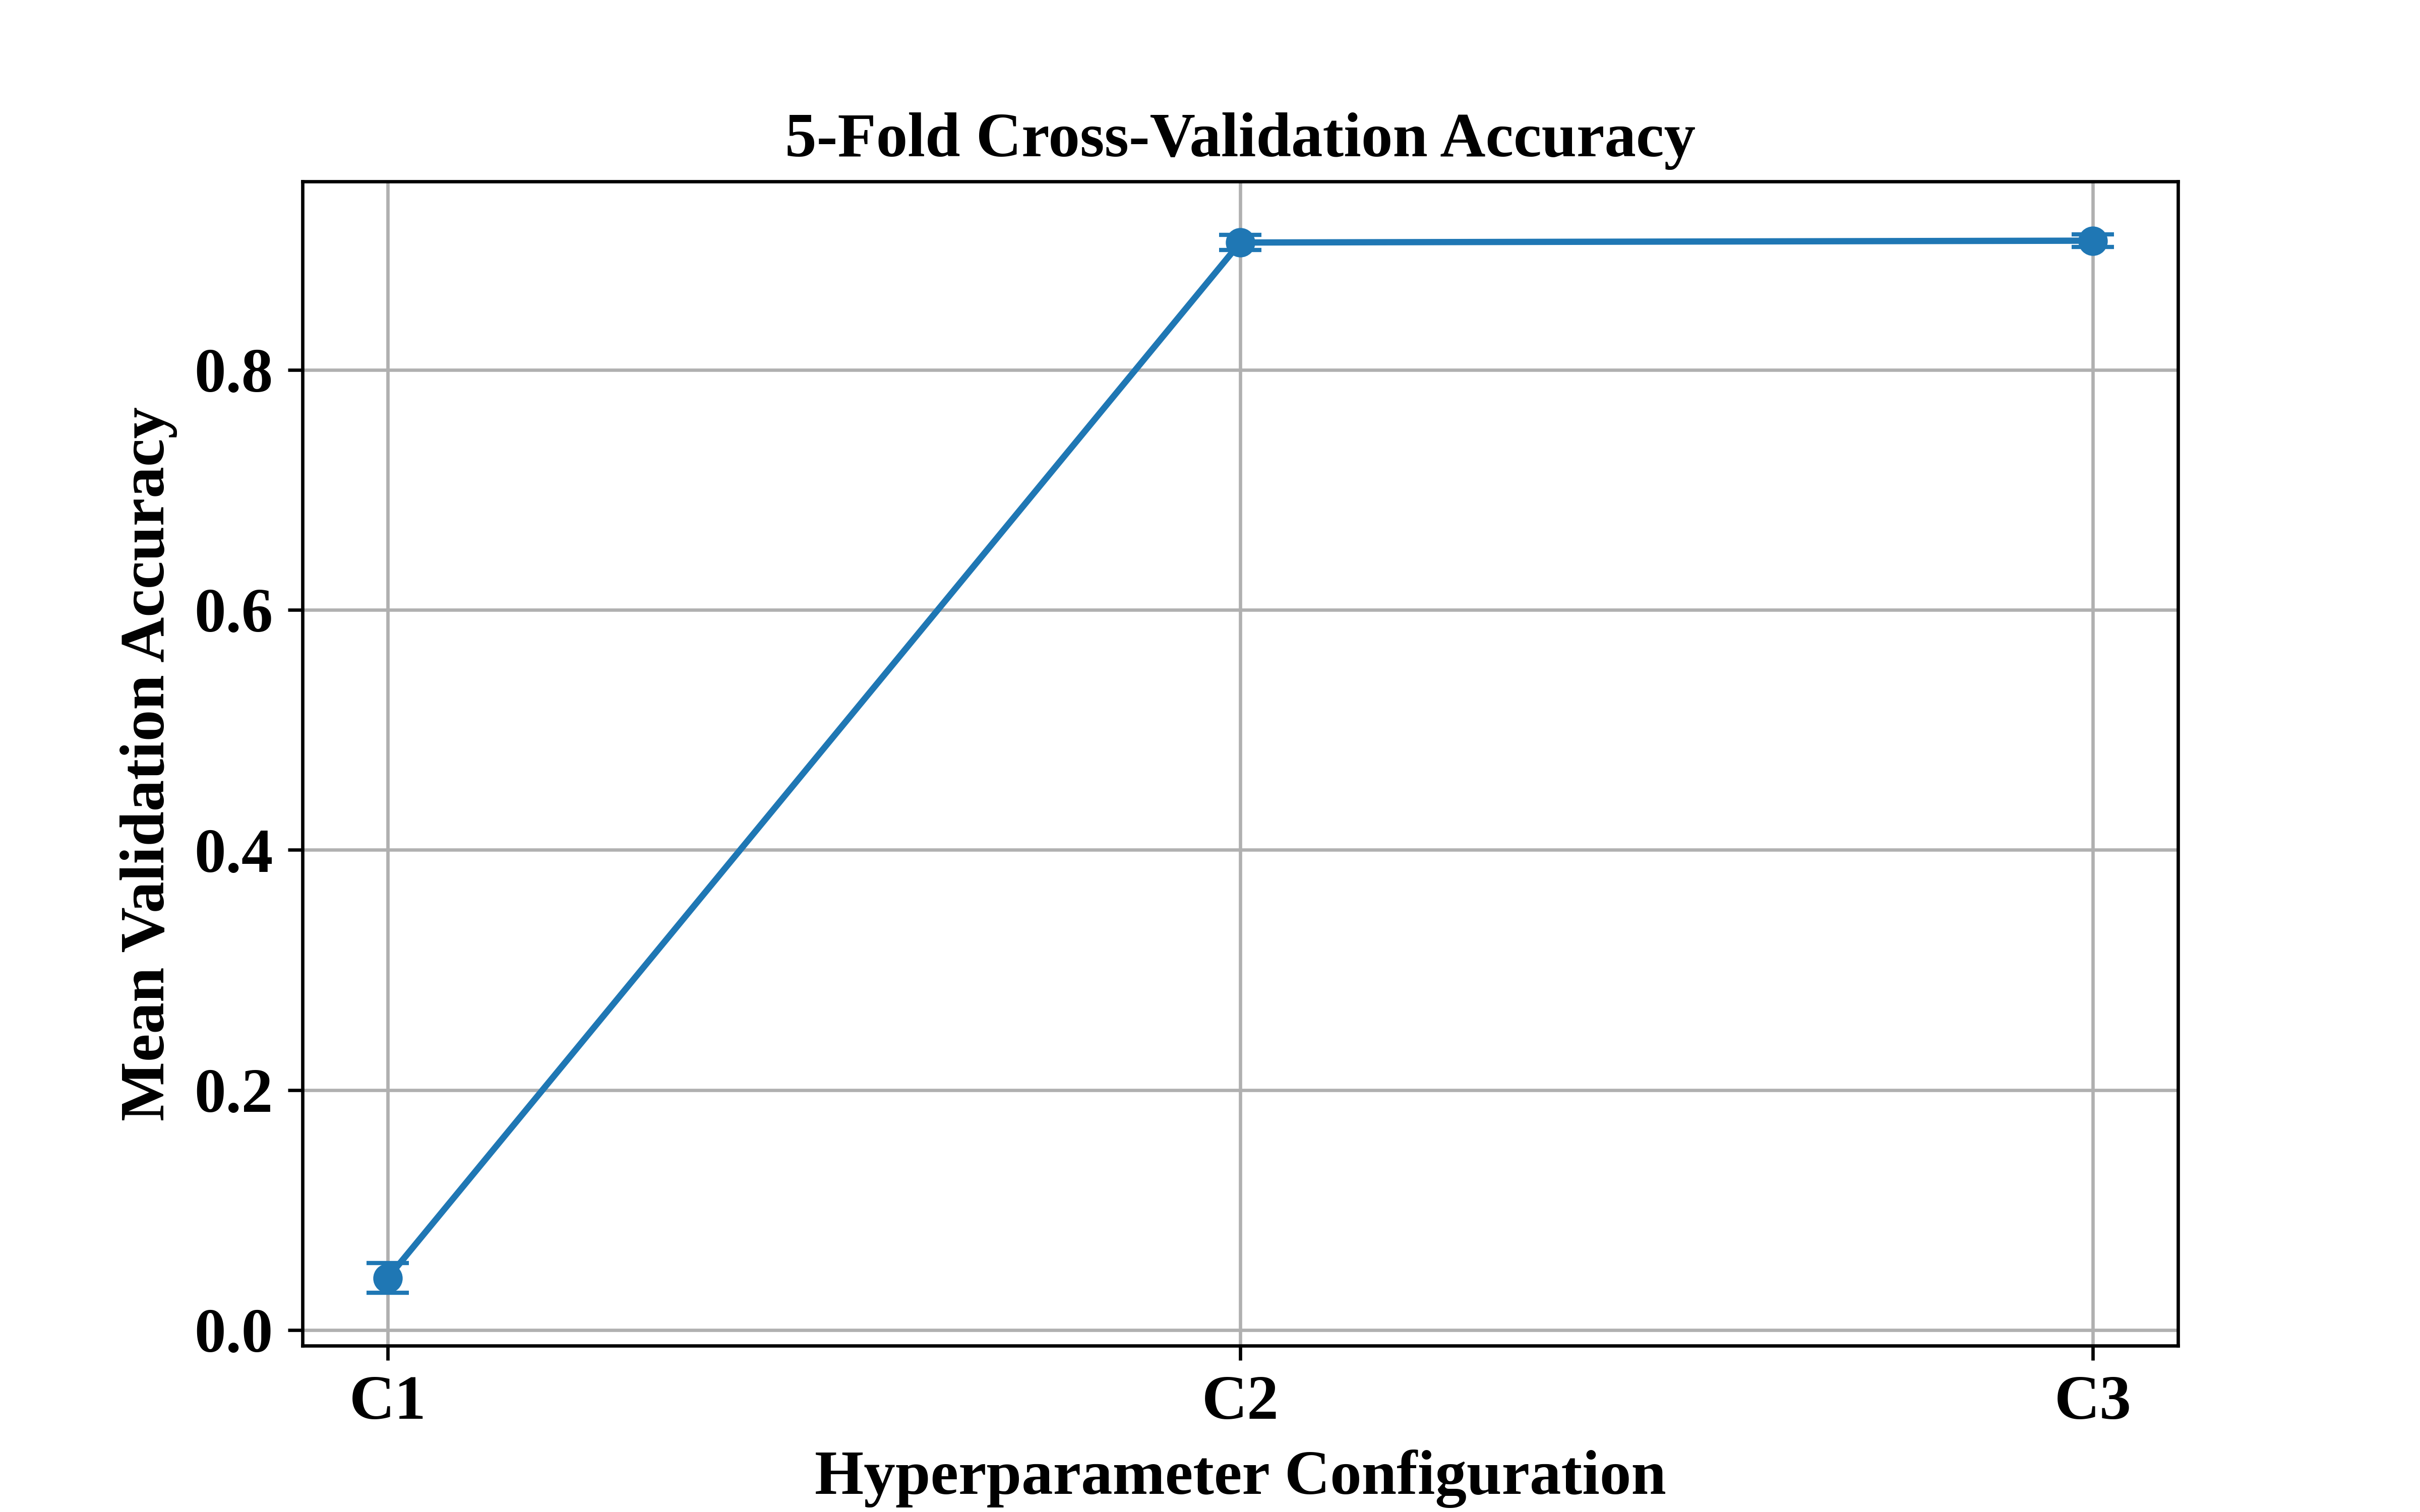
\includegraphics[width=0.8\textwidth]{Images/5FoldCV.png}
        \caption{5-Fold Cross Validation Accuracy}
        \label{fig:5FoldCV}
    \end{figure}
    \noindent\textbf{Inference:}\\
    The plot shows the mean validation accuracy for 3 different hyperparameter configurations.
    C1 has the lowest validation accuracy whereas C3 has the highest validation accuracy.
    The configuration are as follows:

    C1 (Learning rate: 0.0001, Batch size: 16, Dropout:0.25, Optimizer: SGD)

    C2 (Learning rate: 0.001, Batch size: 16, Dropout:0.25, Optimizer: Adam)

    C3 (Learning rate: 0.001, Batch size: 32, Dropout:0.5, Optimizer: Adam)

    C1 performs poorly as it uses SGD optimizer. 
    Whereas Adam adaptively calculates individual learning rates for every parameter using momentum, allowing it to converge faster and require far less manual tuning than SGD.

    \clearpage
    \item\textbf{Confusion Matrix}
        \begin{figure}[H]
        \centering
        
\includegraphics[width=1.1\textwidth]{Images/ConfusionMatrix.png}
        \caption{ConfusionMatrix}
        \label{fig:ConfusionMatrix}
    \end{figure}
    \noindent\textbf{Inference:}\\
    The confusion matrix shows the performance of image classification model on 37 different pet breeds.
    Minor misclassifications are rare and occurs between visually similar pet breeds such as Staffordshire Bull Terriers are misclassified as Pit Bulls and Ragdolls with Birmans.
    This trend occurs because while the model easily learns distinct breed features, closely related breeds share nearly identical physical features.


    \clearpage

    \item\textbf{Misclassified Images}
        \begin{figure}[H]
        \centering
        
\includegraphics[width=0.7\textwidth]{Images/MisclassifiedImages.png}
        \caption{Misclassified Images}
        \label{fig:MisclassifiedImages}
    \end{figure}
    \noindent\textbf{Inference:}\\
    The figure shows some of the images that has been misclassified by the model.
    From the misclassified images, we can see that cat images are mapped to cat breeds, and dog images are mapped to dog breeds.
    However, there has been a class mismatch of cat breeds and dog breeds for cat and dog images respectively.
    It is also observed that a chihuahua has been misclassified as a sphynx which is a cat breed.


\end{enumerate}

\clearpage

%%%%%%%%%%%%%%%%%%%%%%%%%%%%%%%%%%%%%%%%%%%%%%%%%%%%%%%%%%%%\section{Results}
\section{Results}
\textbf{Optimization Algorithms Report}
\vspace{5mm}
\begin{center}
\begin{tabular}{|l|c|c|c|c|}
\hline
Optimizer & Final Loss & Best Val. Accuracy & Epoch to Converge & Training Time (in seconds)\\
\hline
SGD &  3.498174 & 0.066727 & 10 & 219.736567\\
Momentum & 1.418184 & 0.741208 & 10 & 203.661996 \\
RMSProp & 0.122968 &  0.912534 & 8 & 260.758930 \\
Adam & 0.149744 & 0.899008 & 9 & 208.824780\\
\hline
\end{tabular}
\end{center}

\vspace{5mm}

\textbf{K-Fold Cross Validation Report}
\begin{center}
\begin{tabular}{|l|ccccc|c|}
\hline

Configuration &
\multicolumn{5}{c|}{Accuracy} &
Mean $\pm$ SD \\

\cline{2-6}

& Fold 1 & Fold 2 & Fold 3 & Fold 4 & Fold 5 & \\

\hline

C1 & 0.0338& 0.0444& 0.0290 &0.0648 &0.0445 & 0.0433 ± 0.0123 \\
C2 & 0.906280& 0.898551& 0.915861 &0.900387 & 0.909091 & 0.9060 ± 0.0062\\
C3 & 0.899517  & 0.907246 & 0.906190 & 0.909091 & 0.915861 & 0.9076 ± 0.0053 \\
\hline
\end{tabular}
\end{center}

\vspace{5mm}

\textbf{Final Model Evaluation Report}
\vspace{5mm}

\begin{center}
\begin{tabular}[H]{|l|c|}
\hline
Metric & Value\\
\hline
Mean CV Accuracy & 0.907581\\
CV Standard Deviation & 0.005252\\
Test Accuracy & 0.9161406755447388\\
Precision & 0.919625783910535\\
Recall & 0.9161406672678089\\
F1-score & 0.9160590223088639\\
Training Time & 251 seconds\\
Number of Parameters & 2426725\\
\hline
\end{tabular}
\end{center}
\vspace{5mm}

\textbf{Overall Results}
\vspace{5mm}
\begin{center}

\begin{tabular}[H]{|l|c|c|c|c|}
\hline
Configuration & CV Accuracy & SD & Test Accuracy & Training Time\\
\hline

Baseline & 0.8918 & 0.0087 & 0.8952 & 164 seconds\\

Best Initialization & 0.9085 & 0.0069 & 0.9038 & 127 seconds\\

Best Regularization & 0.9333 & 0.0048 & 0.9287 & 137 seconds\\

Best Optimizer & 0.9196 & 0.0061 & 0.9145 & 261 seconds\\

Best Hyperparameters & 0.9254 & 0.0057 & 0.9218 & 250 seconds\\

Fine-Tuned Model & 0.9076 & 0.0053 & 0.9161 & 251 seconds\\

\hline
\end{tabular}

\end{center}
\clearpage
%%%%%%%%%%%%%%%%%%%%%%%%%%%%%%%%%%%%%%%%%%%%%%%%%%%%%%%%%%%%
\section{Discussion Questions}

\begin{enumerate}
\item What is the difference between model parameters and hyperparameters?
\item Why is weight initialization important?
\item Why can zero initialization be problematic for neural networks?
\item Compare Xavier and He initialization.
\item How can training and validation curves be used to identify overfitting?
\item How does Dropout reduce overfitting?
\item What is the purpose of Batch Normalization?
\item Explain the numerical Batch Normalization example.
\item What are the roles of $\gamma$ and $\beta$?
\item Compare SGD, Momentum, RMSProp and Adam.
\item What happens when the learning rate is too large?
\item What happens when the learning rate is too small?
\item What is the effect of increasing batch size?
\item Explain stride and padding.
\item Why is MobileNetV2 computationally efficient?
\item What is depthwise separable convolution?
\item What is transfer learning?
\item Differentiate feature extraction and fine-tuning.
\item Why is a smaller learning rate generally used during fine-tuning?
\item Why is K-Fold Cross-Validation useful for hyperparameter selection?
\item Why must the test set remain untouched during tuning?
\item Why should mean and standard deviation both be reported?
\item Is the highest validation accuracy always sufficient to select a model?
\end{enumerate}

%%%%%%%%%%%%%%%%%%%%%%%%%%%%%%%%%%%%%%%%%%%%%%%%%%%%%%%%%%%%
\section{Additional Exercise}

Select two new combinations of learning rate, dropout, batch size and
fine-tuning strategy. Evaluate them using 5-fold cross-validation and
compare their results with the selected configuration.

Students must justify whether the new configuration is preferable based
on accuracy, standard deviation, computational cost and final test
performance.

%%%%%%%%%%%%%%%%%%%%%%%%%%%%%%%%%%%%%%%%%%%%%%%%%%%%%%%%%%%%
\section{Expected Outcome}

Students should experimentally demonstrate that CNN performance is
strongly influenced by initialization, regularization, optimization and
hyperparameter choices. They should understand the MobileNetV2 architecture,
perform transfer learning and fine-tuning, and select a reliable final
configuration using 5-fold cross-validation.

%%%%%%%%%%%%%%%%%%%%%%%%%%%%%%%%%%%%%%%%%%%%%%%%%%%%%%%%%%%%
\section{References}

\begin{enumerate}
\item Ian Goodfellow, Yoshua Bengio and Aaron Courville,
\emph{Deep Learning}, MIT Press, 2016.

\item Sergey Ioffe and Christian Szegedy,
``Batch Normalization: Accelerating Deep Network Training by Reducing
Internal Covariate Shift,'' ICML, 2015.

\item Mark Sandler, Andrew Howard, Menglong Zhu, Andrey Zhmoginov and
Liang-Chieh Chen, ``MobileNetV2: Inverted Residuals and Linear
Bottlenecks,'' CVPR, 2018.

\item Omkar M. Parkhi, Andrea Vedaldi, Andrew Zisserman and C. V. Jawahar,
``Cats and Dogs,'' IEEE Conference on Computer Vision and Pattern
Recognition, 2012.

\item TensorFlow Documentation:
\url{https://www.tensorflow.org}

\item Keras Documentation:
\url{https://keras.io}
\end{enumerate}

\end{document}